% -*-latex-*-

%% IMPORTANT: The official thesis specifications are available at:
%%            http://libraries.mit.edu/archives/thesis-specs/
%%
%%            Please verify your thesis' formatting and copyright
%%            assignment before submission.  If you notice any
%%            discrepancies between these templates and the
%%            MIT Libraries' specs, please let us know
%%            by e-mailing thesis@mit.edu

%% The documentclass options along with the pagestyle can be used to generate
%% a technical report, a draft copy, or a regular thesis.  You may need to
%% re-specify the pagestyle after you \include  cover.tex.  For more
%% information, see the first few lines of mitthesis.cls.

%\documentclass[12pt,vi,twoside]{mitthesis}
%%
%%  If you want your thesis copyright to you instead of MIT, use the
%%  ``vi'' option, as above.
%%
%\documentclass[12pt,twoside,leftblank]{mitthesis}
%%
%% If you want blank pages before new chapters to be labelled ``This
%% Page Intentionally Left Blank'', use the ``leftblank'' option, as
%% above.

\documentclass[12pt,twoside]{mitthesis}
\usepackage{lgrind}
%% These have been added at the request of the MIT Libraries, because
%% some PDF conversions mess up the ligatures.  -LB, 1/22/2014
\usepackage{cmap}
\usepackage[T1]{fontenc}
\usepackage{indentfirst}
\usepackage[colorlinks=true,bookmarks=true]{hyperref}
\usepackage{bookmark}
\hypersetup{breaklinks=true}
\pagestyle{plain}

%% Addtional packages
\usepackage{amsmath}
\usepackage{amssymb}
\usepackage{array}
\usepackage{caption}
\usepackage{subcaption}
\usepackage{enumitem}
\usepackage{graphicx}
\usepackage{epstopdf}

\usepackage[colorlinks=true,bookmarks=true]{hyperref}
\usepackage{bookmark}
\usepackage[capitalise]{cleveref}
\hypersetup{breaklinks=true}
\usepackage[numbers,sort&compress]{natbib}
\usepackage{physics}
%\usepackage{pict2e}    %problem
\usepackage{setspace}
\usepackage{slashed}
\usepackage{siunitx}   
\usepackage{supertabular}  
\usepackage{textcomp}
\usepackage{url}
\usepackage[usenames]{xcolor}
\usepackage{bm}


%% This bit allows you to either specify only the files which you wish to
%% process, or `all' to process all files which you \include.
%% Krishna Sethuraman (1990).

%\typein [\files]{Enter file names to process, (chap1,chap2 ...), or `all' to process all files:}
%\def\all{all}
%\ifx\files\all \typeout{Including all files.} \else \typeout{Including only \files.} \includeonly{\files} \fi

\begin{document}

\hypersetup{pageanchor=false}
\pagenumbering{roman}
% -*-latex-*-
%
% For questions, comments, concerns or complaints:
% thesis@mit.edu
%
%
% $Log: cover.tex,v $
% Revision 1.8  2008/05/13 15:02:15  jdreed
% Degree month is June, not May.  Added note about prevdegrees.
% Arthur Smith's title updated
%
% Revision 1.7  2001/02/08 18:53:16  boojum
% changed some \newpages to \cleardoublepages
%
% Revision 1.6  1999/10/21 14:49:31  boojum
% changed comment referring to documentstyle
%
% Revision 1.5  1999/10/21 14:39:04  boojum
% *** empty log message ***
%
% Revision 1.4  1997/04/18  17:54:10  othomas
% added page numbers on abstract and cover, and made 1 abstract
% page the default rather than 2.  (anne hunter tells me this
% is the new institute standard.)
%
% Revision 1.4  1997/04/18  17:54:10  othomas
% added page numbers on abstract and cover, and made 1 abstract
% page the default rather than 2.  (anne hunter tells me this
% is the new institute standard.)
%
% Revision 1.3  93/05/17  17:06:29  starflt
% Added acknowledgements section (suggested by tompalka)
%
% Revision 1.2  92/04/22  13:13:13  epeisach
% Fixes for 1991 course 6 requirements
% Phrase "and to grant others the right to do so" has been added to
% permission clause
% Second copy of abstract is not counted as separate pages so numbering works
% out
%
% Revision 1.1  92/04/22  13:08:20  epeisach

% NOTE:
% These templates make an effort to conform to the MIT Thesis specifications,
% however the specifications can change. We recommend that you verify the
% layout of your title page with your thesis advisor and/or the MIT
% Libraries before printing your final copy.

\title{Title}

\makeatletter
\author{John Smith} \let\Author\@author
% If you wish to list your previous degrees on the cover page, use the
% previous degrees command:
%       \prevdegrees{A.A., Harvard University (1985)}
% You can use the \\ command to list multiple previous degrees
%       \prevdegrees{B.S., University of California (1978) \\
%                    S.M., Massachusetts Institute of Technology (1981)}
\prevdegrees{Beijing, China \\
             B.S., University of Virginia (2016) \\
             S.M., University of Virginia (2016)}
\department{Department of A}

% If the thesis is for two degrees simultaneously, list them both
% separated by \and like this:
% \degree{Doctor of Philosophy \and Master of Science}
\degree{Doctor of Philosophy}

% As of the 2007-08 academic year, valid degree months are September,
% February, or June.  The default is June.
\degreemonth{Jan}
\degreeyear{2016} \let\Year\@degreeyear
\thesisdate{Jan 1, 2016}
\makeatother

%% By default, the thesis will be copyrighted to MIT.  If you need to copyright
%% the thesis to yourself, just specify the `vi' documentclass option.  If for
%% some reason you want to exactly specify the copyright notice text, you can
%% use the \copyrightnoticetext command.
%\copyrightnoticetext{\copyright IBM, 1990.  Do not open till Xmas.}

% If there is more than one supervisor, use the \supervisor command
% once for each.
\supervisor{John Smith}{Professor}

% This is the department committee chairman, not the thesis committee
% chairman.  You should replace this with your Department's Committee
% Chairman.
\chairman{N/A}{N/A}

% Make the titlepage based on the above information.  If you need
% something special and can't use the standard form, you can specify
% the exact text of the titlepage yourself.  Put it in a titlepage
% environment and leave blank lines where you want vertical space.
% The spaces will be adjusted to fill the entire page.  The dotted
% lines for the signatures are made with the \signature command.
\makeatletter
\def\maketitle{\begin{titlepage}
\doublespacing
\vspace{0.8in}
\large
{\LARGE\bf \@title \par}
\@author \\
\@prevdegrees
\par
A Dissertation Presented to the Graduate Faculty \\
of the University of Virginia in Candidacy for the Degree of \\
\@degree
\par
\@department
\par
University of Virginia \\
\@degreemonth, \@degreeyear
\vspace{0.8in}
\end{titlepage}}
\makeatother
\maketitle

% The abstractpage environment sets up everything on the page except
% the text itself.  The title and other header material are put at the
% top of the page, and the supervisors are listed at the bottom.  A
% new page is begun both before and after.  Of course, an abstract may
% be more than one page itself.  If you need more control over the
% format of the page, you can use the abstract environment, which puts
% the word "Abstract" at the beginning and single spaces its text.

%% You can either \input (*not* \include) your abstract file, or you can put
%% the text of the abstract directly between the \begin{abstractpage} and
%% \end{abstractpage} commands.

% First copy: start a new page, and save the page number.
% \cleardoublepage
% Uncomment the next line if you do NOT want a page number on your
% abstract and acknowledgments pages.
% \pagestyle{empty}
% \setcounter{savepage}{\thepage}
% \begin{abstractpage}
% % -*-latex-*-
%
% $Log: abstract.tex,v $
% Revision 1.1  93/05/14  14:56:25  starflt
% Initial revision
%
% Revision 1.1  90/05/04  10:41:01  lwvanels
% Initial revision

%% The text of your abstract and nothing else (other than comments) goes here.
%% It will be single-spaced and the rest of the text that is supposed to go on
%% the abstract page will be generated by the abstractpage environment. This
%% file should be \input (not \include 'd) from cover.tex.

\noindent
This is the abstract section. You should replace this with your own abstract.

%%%%%%%%%%%%%%%%%%%%%%%%%%%%%%%%%%%%%%%%%%%%%%%%%%%%%%%%%%%%%%%%%%%%%%
% -*-latex-*-

% \end{abstractpage}

% Additional copy: start a new page, and reset the page number.  This way,
% the second copy of the abstract is not counted as separate pages.
% Uncomment the next 6 lines if you need two copies of the abstract
% page.
% \setcounter{page}{\thesavepage}
% \begin{abstractpage}
% % -*-latex-*-
%
% $Log: abstract.tex,v $
% Revision 1.1  93/05/14  14:56:25  starflt
% Initial revision
%
% Revision 1.1  90/05/04  10:41:01  lwvanels
% Initial revision

%% The text of your abstract and nothing else (other than comments) goes here.
%% It will be single-spaced and the rest of the text that is supposed to go on
%% the abstract page will be generated by the abstractpage environment. This
%% file should be \input (not \include 'd) from cover.tex.

\noindent
This is the abstract section. You should replace this with your own abstract.

%%%%%%%%%%%%%%%%%%%%%%%%%%%%%%%%%%%%%%%%%%%%%%%%%%%%%%%%%%%%%%%%%%%%%%
% -*-latex-*-

% \end{abstractpage}

% Copyright page
\pagestyle{empty}
\newpage
\vspace*{\fill}
\noindent \textcopyright Copyright by \Author {} \Year \\
All Rights Reserved

\cleardoublepage

% Abstract page
\vspace{0.8in}
\pdfbookmark[0]{Abstract}{Abstract}
\section*{\center Abstract}
% -*-latex-*-
%
% $Log: abstract.tex,v $
% Revision 1.1  93/05/14  14:56:25  starflt
% Initial revision
%
% Revision 1.1  90/05/04  10:41:01  lwvanels
% Initial revision

%% The text of your abstract and nothing else (other than comments) goes here.
%% It will be single-spaced and the rest of the text that is supposed to go on
%% the abstract page will be generated by the abstractpage environment. This
%% file should be \input (not \include 'd) from cover.tex.

\noindent
This is the abstract section. You should replace this with your own abstract.

%%%%%%%%%%%%%%%%%%%%%%%%%%%%%%%%%%%%%%%%%%%%%%%%%%%%%%%%%%%%%%%%%%%%%%
% -*-latex-*-


\cleardoublepage

% Acknowledgemnt page
\pagenumbering{roman}
\pagestyle{plain}
\pdfbookmark[0]{Acknowledgments}{Acknowledgments}
\section*{Acknowledgments}
% -*-latex-*-

%% The text of your acknowledgement and nothing else (other than comments)
%% goes here. It will be single-spaced and the rest of the text that is
%% supposed to go on the acknowledgement page will be generated by the
%% abstractpage environment. This file should be \input (not \include 'd)
%% from cover.tex.

This is the acknowledgement section.
\par
You should replace this with your own acknowledgements.

%%%%%%%%%%%%%%%%%%%%%%%%%%%%%%%%%%%%%%%%%%%%%%%%%%%%%%%%%%%%%%%%%%%%%%
% -*-latex-*-


%%%%%%%%%%%%%%%%%%%%%%%%%%%%%%%%%%%%%%%%%%%%%%%%%%%%%%%%%%%%%%%%%%%%%%
% -*-latex-*-

\hypersetup{pageanchor=true}

\hypersetup{linkcolor=black}
\pagestyle{plain}
% -*-latex-*-

%% This file simply contains the commands that actually generate the table of
%% contents and lists of figures and tables.  You can omit any or all of
%% these files by simply taking out the appropriate command.  For more
%% information on these files, see appendix C.3.3 of the LaTeX manual.

\cleardoublepage
\pdfbookmark[0]{\contentsname}{Contents}
\tableofcontents
\cleardoublepage
\pdfbookmark[1]{List of Figures}{List of Figures}
\listoffigures
\cleardoublepage
\pdfbookmark[1]{List of Tables}{List of Tables}
\listoftables
\cleardoublepage

%%%%%%%%%%%%%%%%%%%%%%%%%%%%%%%%%%%%%%%%%%%%%%%%%%%%%%%%%%%%%%%%%%%%%%
% -*-latex-*-

\hypersetup{linkcolor=red}

\pagenumbering{arabic}
% -*-latex-*-

%% This is an example first chapter.  You should put chapter/appendix that you
%% write into a separate file, and add a line \include{yourfilename} to
%% main.tex, where `yourfilename.tex' is the name of the chapter/appendix file.
%% You can process specific files by typing their names in at the
%% \files=
%% prompt when you run the file main.tex through LaTeX.

\chapter{Introduction}
\label{Introduction}


\section{High Energy Electron Scattering}
%Rise the question! The history of QCD, traditional nuclear physics

%In 1911, Ernest Rutherford formulated his model of atom by interpreting the data of his gold foil experiment: a dense
%charged nucleus containing most of atom's mass, was surrounded by an electron cloud.

%As time went on, it was found that nucleus itself is composed of more fundamental particles which are called nucleons.
%Nucleons are the building blocks of the traditional nuclear physics. The properties of free nucleons have been studied
%quite well.
%However, in nuclei, nucleons are in bound state and their properties will be affected by the nuclear medium.
%The question of how nuclear medium will change the properties of nucleons is of great interest and yet still unsolved.
%

Quantum chromodynamics, or QCD, is the theory that describes the action of the strong force that binds quarks together to form baryons and
mesons, and results in the complicated the force that binds atomic nucleon together. QCD is successful in the very high energy (short distance) domain
i.e. weak coupling regime, in which a perturbative approach is valid. On the other hand, traditional nuclear physics theories work well in the
low energy (long range) domain. However, in the medium-high energy region around 1 GeV, techniques of perturbative QCD are invalid and both
QCD and traditional nuclear physics have major difficulties. A fundamental question in nuclear physics is: How can one place the low energy theories
and high energy theory (QCD) into a more general frame, on the basis of a fundamental theory? How does one connect the descriptions of long range
and short range phenomena? To answer the questions, it is essential to understand the phenomena in the medium-high energy region. Building a
bridge between nuclear physics and particle physics is an important step in the progress of physics.

The building blocks of traditional nuclear physics are nucleons. To study the structure and properties of nuclei, we
need to understand the hehaviors of nucleons in nuclei. The properties of free nucleons have been studied very well.
But nucleons in nuclei are in bound states, and their properties will be affected by nuclear medium.
How medium modifications of the nucleon form factor inside the nuclei is an essential question in nuclear physics.

To investigate the properties of nucleons in nuclear medium, the electron is used as a probe, which has several 
advantages over hadrons. The interaction between the electron and nuclei is much weaker than strong interaction.
So the electron will not disturb the nucleus as much as a hadron probe, so the physics is easier to study compare
with the more complicated nucleus-probe system.
Besides, the electron probe interact with the electro-magnetic interaction, which is very well understood through
Quantum Electrodynamics (QED). So electron probe can provide us the most useful information about nucleon and nuclear
structure.

\section{Inclusive Electron Scattering Spectrum}

Figure.~\ref{fig:scattering_spectrum}  shows a cross section spectrum for a typical inclusive scattering a nuclear target.
In inclusive scattering, only the scattered electron's energy and momentum are measured by detectors.

\begin{figure}[h]
\centering
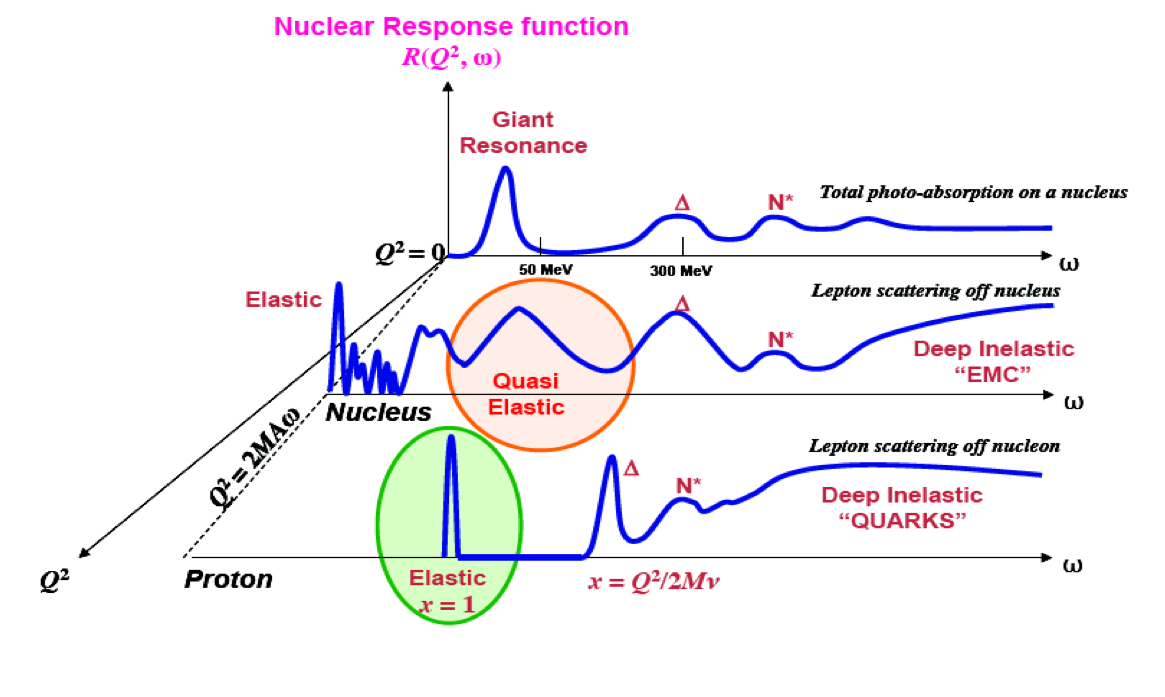
\includegraphics[width=0.8\textwidth]{figs/scattering_spectrum.png}
\caption[scattering spectrum]{Nuclear responses to electron scattering \label{fig:scattering_spectrum}}
\end{figure}

In electron inclusive scattering, as the energy loss $\omega$ increase, different nuclear response structures can
be observed.
The nuclear response structures can be classified as: elastic peak, nuclear excitation levels, giant resonance,
quasi-elastic peak, meson exchange currents (MEC), $\Delta$ peak, higher resonances, and deep inelastic scattering
(DIS).

The first structure can be seen is the elastic peak at $\omega = Q^2/2M$( $Q$ is four momentum transfer and $M$ is the
nucleus mass), the electron's energy loss equal to recoil energy of nucleus.
When the electron's energy loss is larger than the recoil energy, the nucleus will go into an excitation state.
These excitation states correspond to the excitation peaks in the spectrum.

When the energy loss is large enough the electron can knock out a single nucleon from the nucleus, this correspond to
the quasi-elastic peak in the energy loss spectrum. The quasi-elastic peak is a broad peak located above $Q^2/2M_N$ ($M_N$
is the mass of nucleon), the shift of center of the quasi-elastic peak from $Q^2/2M_N$ is due to the average
separation energy. The nucleon motion in nucleus will cause the quasi-elastic peak broadening, and the width of the peak
is characterized by Fermi momentum $k_F$ and momentum transfer $|\vec{q}|$.

If the energy loss continue increase, the knocked out nucleon will be excited into a $\Delta$ resonance state. 
%The $\Delta$ peak is much broader than quasi-elastic peak. 
After the $\Delta$ resonance, there is deep inelastic region and continuum states.

%models, longitudinal and transverse response function

\section{Quasi-elastic Electron Scattering}

In an quasi-elastic inclusive unpolarized electron nucleus scattering process, an electron with initial energy $E$ and
momentum $\vec{k}$ scattered off a rest nucleus of mass $M_N$.
The scattered electron is then measured at angle $\theta$ with scattered energy $E'$ and momentum $\vec{k'}$ by detector package.
The process happens with the exchange of a virtual photon $\gamma (\omega, \vec{q})$,
where $\omega = E - E'$, $\vec{q} = \vec{k} - \vec{k'}$ .
%The Feynman diagram of this process at lowest order of $\alpha$ and with plane wave impulse approximation is show in Figure.~\ref{fig:quasi-elastic_diagram}.

\begin{figure}[h]
\centering
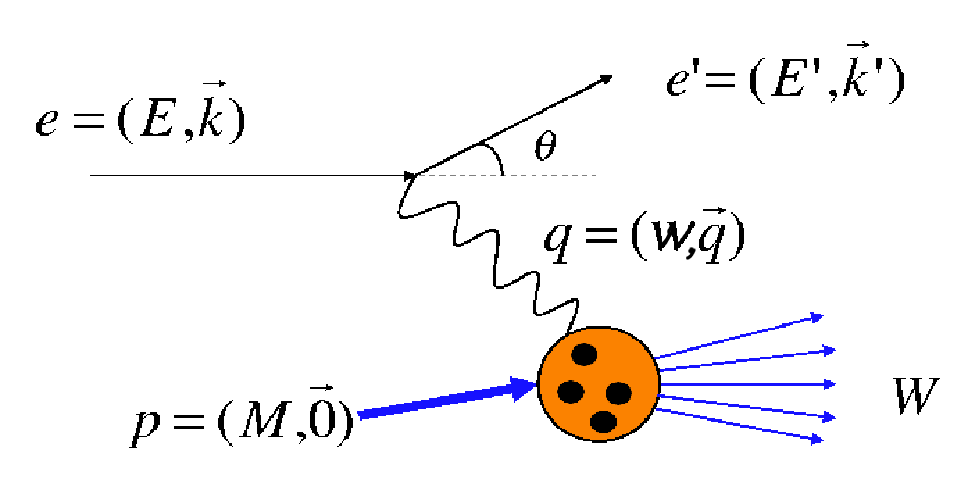
\includegraphics[width=0.8\textwidth]{figs/feynman_diagram.png}
\caption[scattering spectrum]{Quasi-Elastic electron scattering \label{fig:feynman_diagram}}
\end{figure}

With the Born approximation, the differential cross section of the inclusive unpolarized electron scattering described above can be written as:
\begin{equation}
%  \sigma \equiv \frac{d\sigma}{d\Omega d\omega} = \sigma_M [\frac{Q^ 4}{\bm{q}^4}R_L(|\bm{q},\omega|)+\frac{Q^2}{2\bm{q}^2}\frac{R_T(|\bm{q},\omega|)}{\varepsilon}]
%  \sigma \equiv \frac{d\sigma^3}{d\Omega d\omega} = \sigma_M \left[ W_2(|q|,\omega) + 2W_1(|q|,\omega)\tan^2\left(\frac{\theta}{2}\right) \right]
\frac{d\sigma^3}{d\Omega d\omega} = \sigma_M \left[ W_2(|q|,\omega) + 2W_1(|q|,\omega)\tan^2\left(\frac{\theta}{2}\right) \right]
\end{equation}


\begin{equation}
  \sigma_M=\frac{4\alpha^2 \cos^2(\theta/2)}{4E^2\sin^4(\theta/2)}
\end{equation}

is the  Mott cross-section for scattering electrons from a point-like infinitely heavy target. 
It is convenient to separate contribution of longitudinal and transverse polarized virtual photon:
%The right side of this equation can also be re-written to separate contributions of longi- tudinally and transversely polarized virtual photons to the scattering processes
\begin{equation}
\frac{d\sigma^2}{d\Omega d\omega} =  \sigma_M \left[ \frac{Q^4}{\vec{q}^4}R_L(|\vec{q},\omega|)+\frac{Q^2}{2\vec{q}^2\varepsilon}R_T(|\vec{q},\omega|) \right]
\end{equation}


where 

\begin{equation}
Q^2 = \vec{q}^2 - \omega^2
\end{equation}

gives the four momentum squared of the exchanged virtual photon;

\begin{equation}
  \varepsilon(|\vec{q}|,\omega,\theta) =\left[1+\frac{2\vec{q}^2}{Q^2}\tan^2\frac{\theta}{2}\right]^{-1}
\end{equation}

is virtual photon polarization.
This is the Rosenbluth formula.
%a brief derivation is provided in Appendix A for reader's convenience.

The relation of $R_L$ and $R_T$ with $W_1$ and $W_2$ is given by: 
\begin{equation}
R_T(|\vec{q}|)=2W_1(|\vec{q}|)
\end{equation}

and

\begin{equation}
\frac{Q^2}{|\vec{q}|^2}R_L(|\vec{q}|)=W_2(|\vec{q}|) - \frac{Q^2}{|\vec{q}|^2}W_1(|\vec{q}|)
\end{equation}

$R_L$ is the longitudinal response function, $R_T$ is the transverse response function of nucleus.
$R_L$ measures the nuclear charge and $R_T$ measures the magnetic component of the electromagnetic current of the
nucleus. Experimentally the $R_L$ and $R_T$ can be extracted by measuring cross section at a given $(Q^2,\omega)$ at
two or more angles. Then a plot of $\varepsilon \frac{d\sigma^2}{d\Omega d\omega}/\sigma_M$ vesus $\varepsilon$ should 
fall on a straight line. The slope of this line is $(Q^4/\vec{q}^4)R_L$, the intercept is $(Q^2/2\vec{q}^2)R_T$.

\section{Coulomb Sum Rule}

The Coulomb Sum is defined as the integration of longitudinal response function $R_L(|\vec{q}|,\omega)$ divided by 
nucleon charge form factor over the full range of energy loss $\omega$ at a constant three momentum transfer $q \equiv |\vec{q}|$:

\begin{equation}
C_{in}(q) = \int_{\omega_{el}^{+}}^{q} \frac{R_L(|q|,\omega)}{F_1^2(Q^2)} d\omega = Z + \Delta C
\end{equation}

where $F_1^2(Q^2)$ is nucleon charge form factor. $\omega_{el} = Q^2/2M$, $\omega_{el}^{+}$ mean just above the elastic peak. 
Z is the charge number of the target nucleus, and $\Delta C$ is the two-nucleon correlation function.

The relativistic effects and the neutron contributions can be considered as corrections:
\begin{equation}
\tilde{G}^2_E = |\tilde{G}^p_E(Q^2)|^2 + (N/Z) |\tilde{G}^n_E(Q^2)|^2
\end{equation}

\begin{equation}
\tilde{G}^{p(n)}_E(Q^2) = G^{p(n)}_E(Q^2) \sqrt{\frac{1+Q^2/4m^2_N}{1+Q^2/2m^2_N}}
\end{equation}

where $m_N$ is the nucleon mass, N is the neutron number of the nucleus, and $G^{p(n)}_E$ is the proton (neutron)
charge form factor.

At high momentum transfer, another form of Coulomb sum is defined:

\begin{equation}
S_L(Q^2) = \int_{\omega_{el}^{+}}^{\omega_{max}} \frac{R_L(Q^2,\omega)}{|\tilde{G}_E(Q^2)|^2}
\end{equation}

where $\omega_{max}$ is the maximum value of the energy defined by the virtual mass of the exchanged photon:
$\omega < |\vec{q}|$. Here we define $S_L$ as a function of $Q^2$ instead of $|\vec{q}|$, because $Q^2$
a Lorentz invariant.Since it is defined only in the physical region
($Q^2>0$), the problem of strength from outside the physically accessible region is
also avoided.

$S_L$ is predicted to be unity, when $q \gg k_f$, $k_f$ is the fermi momentum of the nucleus.
%However, modifications in the electromagnetic properties of the free nucleons by
%the nuclear medium (EMC effect) and the presence of short range correlations can change
%this result. It is generally accepted that $S_L$ shouldn't quench more than a few percent
%at $q = 2k_f$ and reach 1 at higher $q$ values. The validity of reaching unity at high $q$
%is model independent. 
Here are a few corrections to Coulomb Sum Rule:

\begin{itemize}
\item Finite size effect:  
The finite size effect is due to center-of-mass motion. The total Coulomb Sum is not affected by the center-of-mass
correlations,but in actual calculation of CSR one is faced with the difficulty of subtracting spurious center-of-mass 
effect from the nuclear charge form factor.
This effect become smaller with increasing mass number, as shown in Figure.~\ref{fig:finite_size_data}. And this correction is important for
small $q$. 

\begin{figure}[h]
\centering
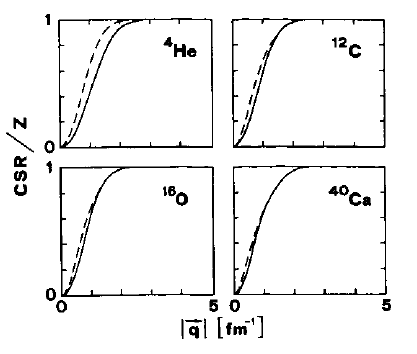
\includegraphics[width=0.7\textwidth]{figs/finite_size_data.png}
\caption[finite size data]{CSR divided by the proton number, as a function of the three-momentum transfer, in the
harmonic oscillator model, without(broken curve) and with(full curve) center-of-mass corrections. Figure from
\cite{Orlandini1991}.  \label{fig:finite_size_data}}
\end{figure}


\item Pauli blocking: The nucleons are fermions, and the Pauli exclusion principle requires that two or more nucleons
cannot occupy the same quantum state within the same quantum system. 
The Pauli blocking is more important at small $|\vec{q}|$ and negligible at large $|\vec{q}|$. The comparison between
with and without Pauli correlations is calculated by Lightbody using harmonic oscillator model for $^{12}C$ is shown
in Figure.\ref{fig:pauli_blocking_compare}.

\begin{figure}[h]
\centering
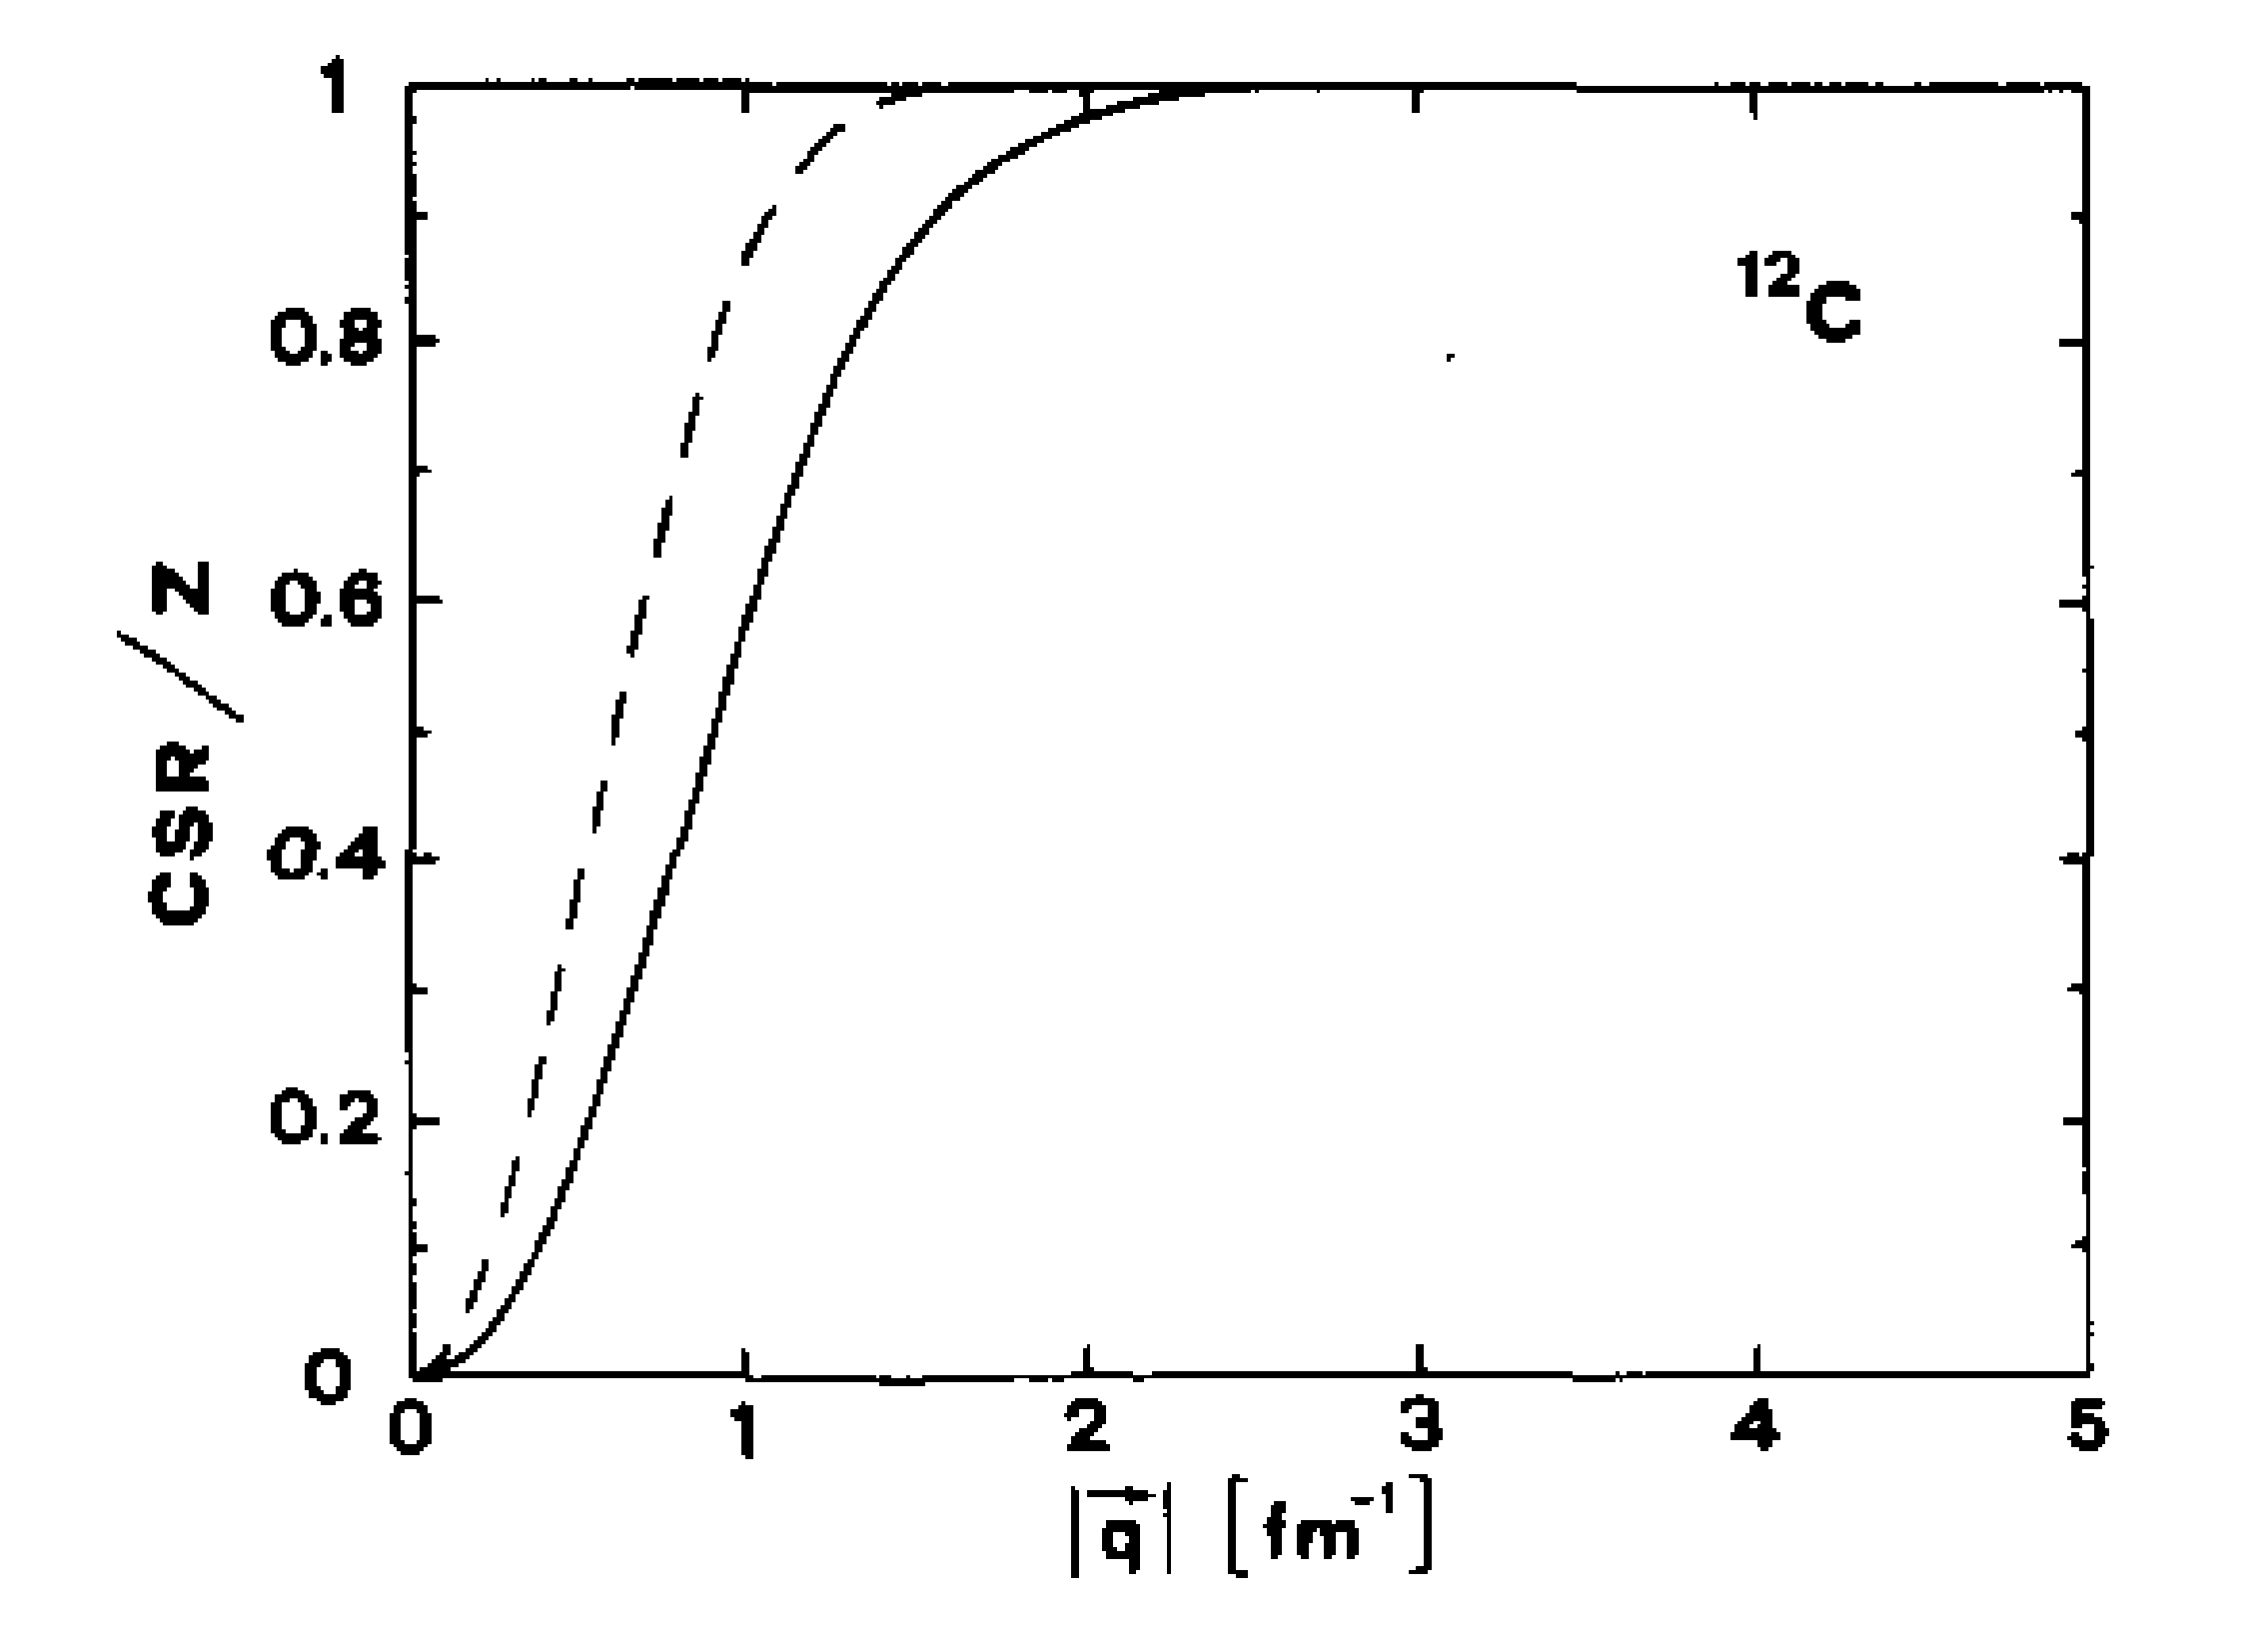
\includegraphics[width=0.7\textwidth]{figs/pauli_blocking_compare.png}
\caption[pauli blocking compare]{CSR divided by the proton number, as a function of the three momentum transfer,
without(broken curve) and with(full curve) Pauli correlations. Figure from
\cite{Orlandini1991}.  \label{fig:pauli_blocking_compare}}
\end{figure}

\item Long range correlations:
In the region of low momentum transfer, the interaction between nucleons have a long range nature and are responsible
for the giant resonances. The long-range correlation has been studied based on the random phase approximation (RPA).
The long range correlations are effective at low $q$ and vanish at high $q$.
The quenching effect on the CSR produced by the RPA is shown in Figure\ref{fig:long_range_data}:

\begin{figure}[h]
\centering
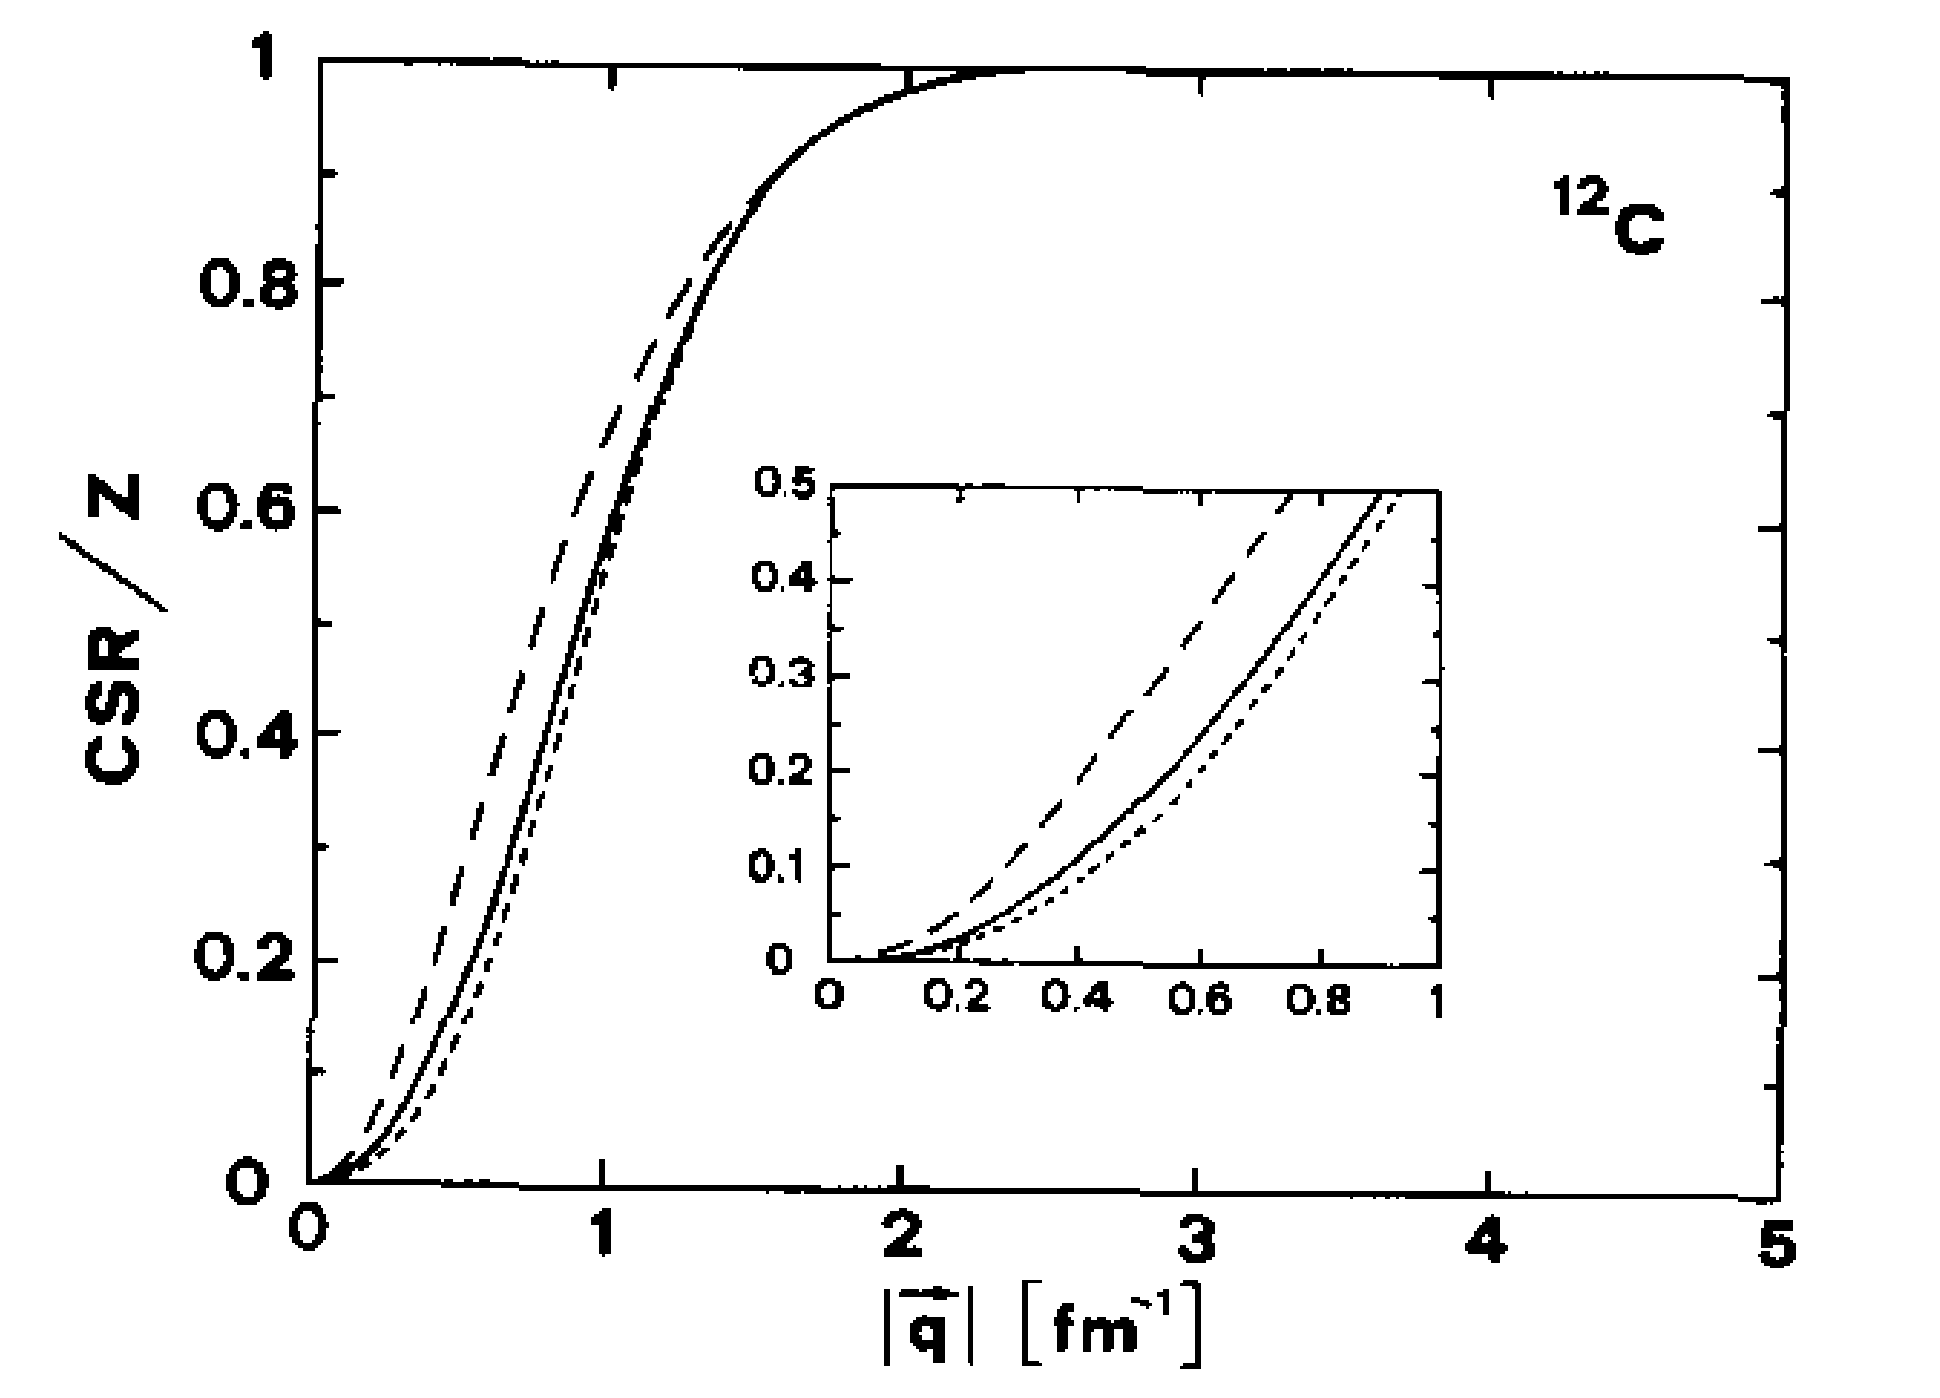
\includegraphics[width=0.7\textwidth]{figs/long_range_data.png}
\caption[long range data]{CSR divided by the proton number, as a function of the three momentum transfer in the 
harmonic oscillator model wihtout (long broken curve) and with(full curve) center-of-mass correlations.
The short broken curve represents the result including RPA correlations.
 Figure from \cite{Orlandini1991}.
\label{fig:long_range_data}}
\end{figure}

\item Short range correlations:
In the deep inelastic (DIS) region, the virtual photon explores the medium and short inter-nucleon distances \cite{Orlandini1991}.
So the longitudinal structure function is sensitive to the short range proton-proton correlations, and these can affect
the CSR to be quenched. Short-range correlations are obtained for example by modifying the
short-range behaviour of the relative proton-proton wavefunction through a Jastrow-type correlation:

\begin{equation}
g(r) = 1 - e^{\gamma \alpha^2 r^2/4}
\end{equation}

The effect of short range correlation for $^{12}$C is shown in Figure\ref{fig:short_range_data}:

\begin{figure}[h]
\centering
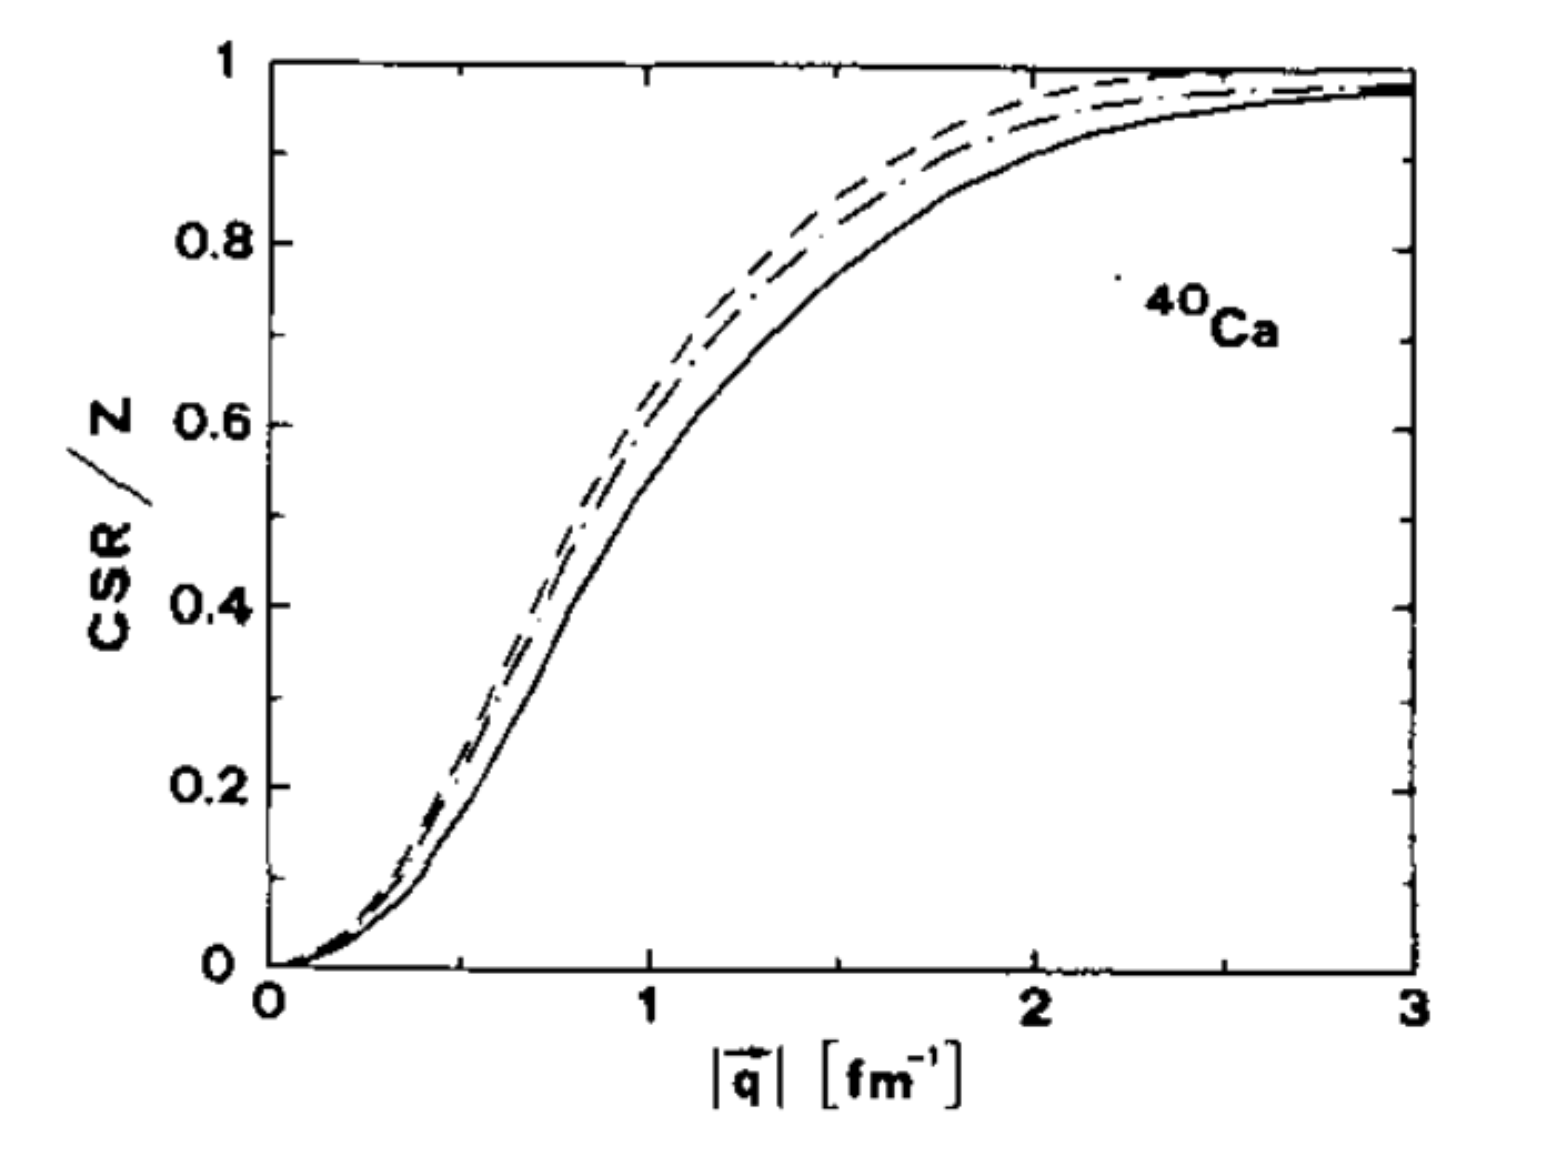
\includegraphics[width=0.7\textwidth]{figs/short_range_data.png}
\caption[short range data]{CSR divided by the proton number, as a function of the three momentum transfer in the 
harmonic oscillator model (broken curve, $\alpha_0$ = 0.51 fm$^{-1}$) and with short-range correlations included
(chain curve, $\gamma$ = 56.1; full curve: $\gamma$ = 24.9).
 Figure from \cite{Orlandini1991}.
\label{fig:short_range_data}}
\end{figure}

\end{itemize}

\section{Existing Data}
In the past thirty years, a large experimental program has been carried out at the Bates, Saclay and SLAC
aimed at the extraction of $R_L$ and $R_T$ for a variety of nuclei \cite{Meziani2001}.
The Bates and Saclay data have the resenbluth separation only performed up to $q$ = 550 MeV/c due to the maximum beam
energy limiation (~800 MeV). At SLAC only a measurement at $q$ = 1140 MeV/c was performed due to the minimum beam energy
available (~900 MeV). The large uncertainty on the SLAC data point makes it inconclusive. So experiment E05-110 at
Jefferson Lab can test Coulomb Sum Rule in the region not measured before with significantly improved precision.

The longitudinal and transverse response functions extracted with Rosenbluth separation are available for
$^2$H, $^3$H, $^3$He, $^4$He, $^{12}$C, $^{40}$Ca, $^{48}$Ca, $^{56}$Fe, $^{238}$U in the range 200 MeV/c $\leq q \leq$
600 MeV.

The experimental transverse response functions are generally in reasonable agreement with the simple model predictions.
In the kinematic region where the contributions from processes such as elastic scattering, nuclear
excitation and giant resonance are small, the agreement between theories and experiments is good.
In the region where the contributions from the other processes, such as meson exchange current (MEC) and $\Delta$ excitation are important,
the situation becomes complicated. By taking into account these contributions, theorists can still reproduce the transverse response function well.

\begin{figure}[h]
\centering
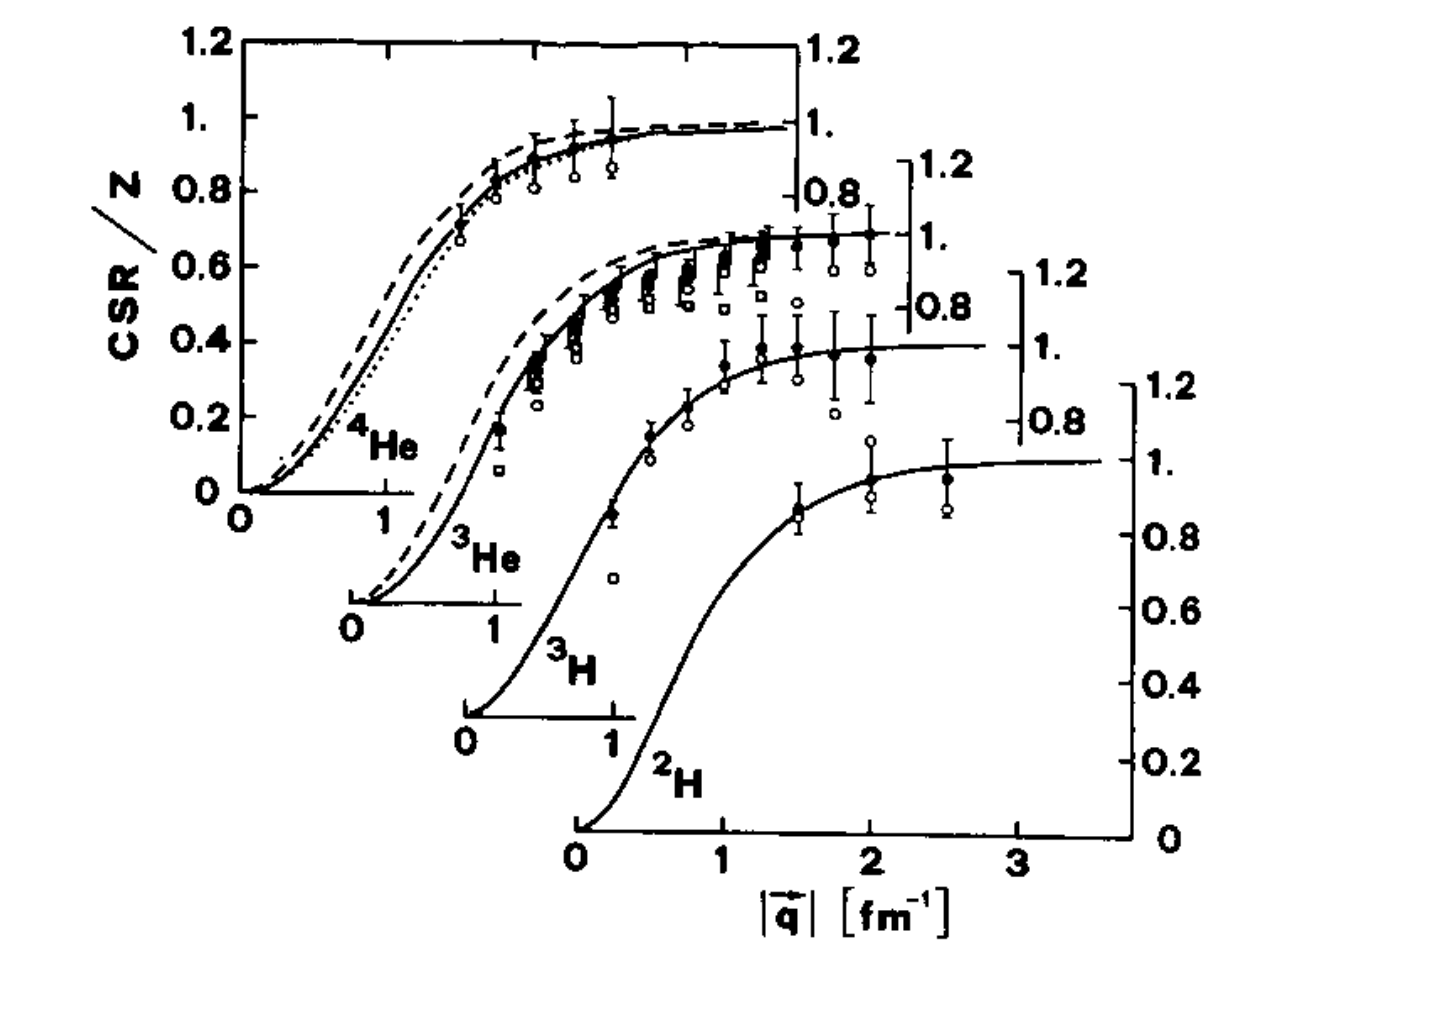
\includegraphics[width=0.7\textwidth]{figs/csr_data.png}
\caption[csr data]{The CSR divided by the proton number as a function of three momentum transfer
for light weight nuclei. Continuous curves: results from Schiavilla \cite{Schiavilla1987} ; dotted curve:
correlated model. The empty points represent the experimental values, while the filled points
are the tail corrected results. Both Saclay (circles) and Bates (squares) data are shown for $^3$He.
 Figure reproduced from \cite{Orlandini1991}.
\label{fig:csr_data}}
\end{figure}

\begin{figure}[h]
\centering
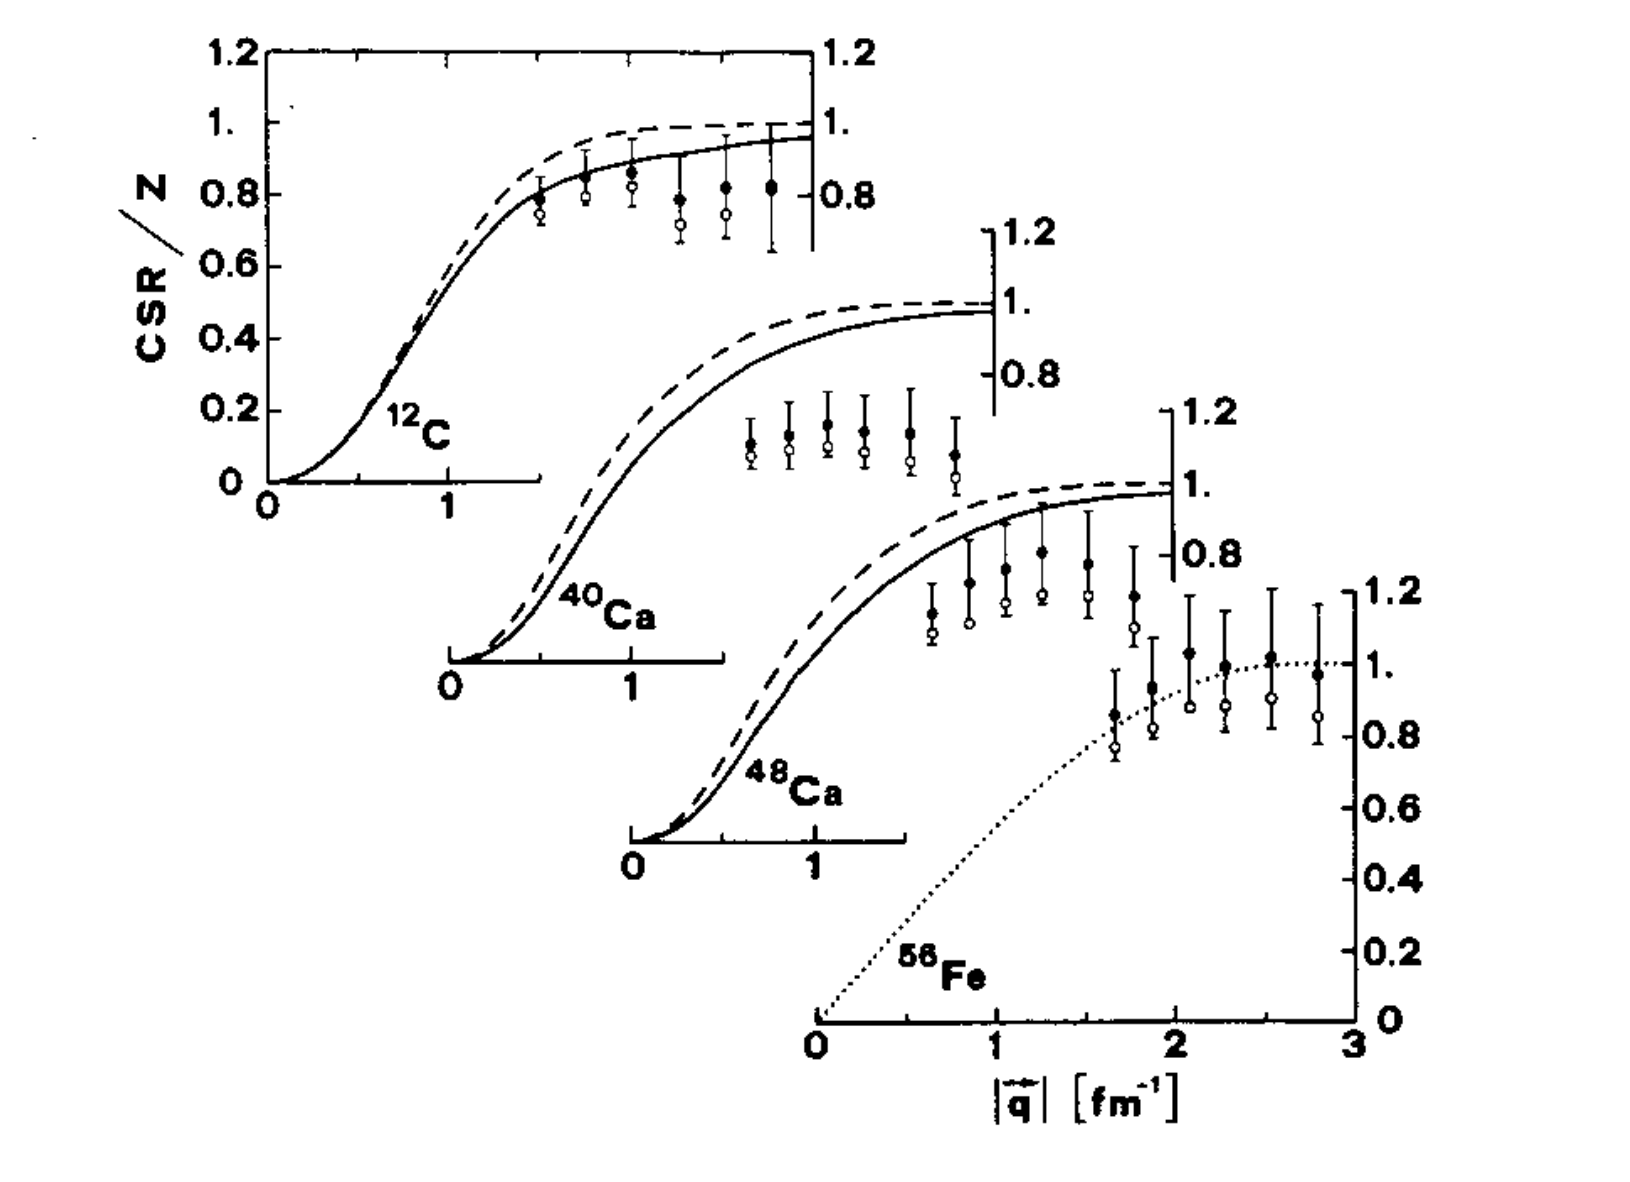
\includegraphics[width=0.7\textwidth]{figs/csr_data_2.png}
\caption[csr data2]{The CSR divided by the proton number as a function of three momentum transfer
for medium weight nuclei. Broken curves: harmonic oscillator; Continuous curves: correlated
model; Dotted curve: Fermi gas model, $k_f$ = 1.32 fm$^{-1}$. The empty points represent the
experimental values from Saclay, while the filled points are the tail corrected results.
 Figure reproduced from \cite{Orlandini1991}.
\label{fig:csr_data2}}
\end{figure}

For the longitudinal response function, the agreement between calculation and experiment is reasonably good
for light nuclei, such as $^2$H, $^3$H, $^3$He. For medium-weight to heavy nuclei(Figure \ref{fig:R_LT_q_410}
,\ref{fig:R_LT_q_550}),
there is an obvious
quenching for the experimental longitudinal response function. The quenching of $R_L$ has a clear
dependence on the nuclear mass number $N$. Besides, the quenching has a dependence on the momentum transfer:
the discrepancy between experimental $R_L$ and simple Fermi gas model calculation becomes smaller when $q$
increases. This feature can be explained by the Pauli correlation, which decrease quickly when $q$ increases.


\begin{figure}
\begin{subfigure}{.7\textwidth}
\centering
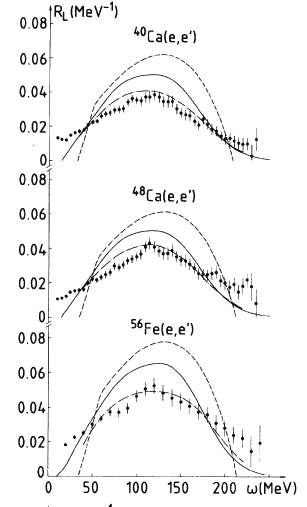
\includegraphics[width=.8\linewidth]{figs/R_L_q_410.png}
\label{fig:R_L_q_410}
\end{subfigure}%
\begin{subfigure}{.5\textwidth}
\centering
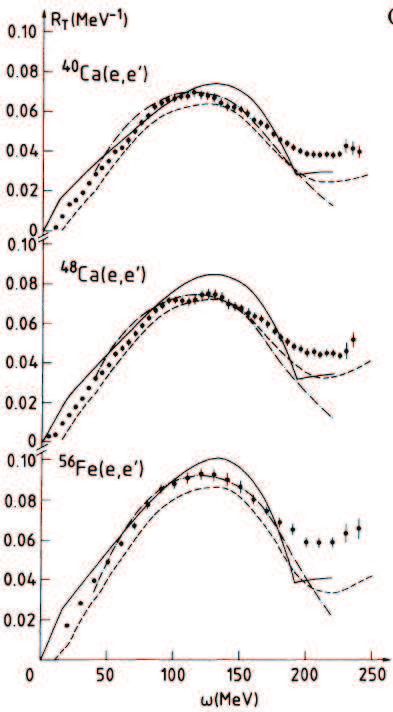
\includegraphics[width=.8\linewidth]{figs/R_T_q_410.png}
\label{fig:R_T_q_410}
\end{subfigure}
\caption[R LT q 410]{
(a) $R_L$ and (b) $R_T$ of $^{40}$Ca, $^{48}$Ca, and $^{56}$Fe at $|\vec{q}|$ = 410 MeV/c.
(a) The dashed line is a Fermi-gas caculation by Van Orden; the solid
line, a shell model calculation by Laget; and the dot deshed line a calculation
by Do Dang. (b) The dashed line is the total contribution from calculation
by Laget. The dot-dashed line is the Do Dang and Va Giai calculation
containing only the quasi-elastic process. The solid line is the random-
phase approximation (RPA) calculation with 1p-1h and 2p-2h excitations
by Alberico, Ericson, and Molinari.
\label{fig:R_LT_q_410}}
\end{figure}


\begin{figure}
\begin{subfigure}{.7\textwidth}
\centering
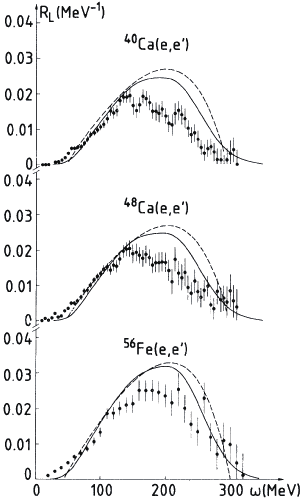
\includegraphics[width=.8\linewidth]{figs/R_L_q_550.png}
\label{fig:R_L_q_550}
\end{subfigure}%
\begin{subfigure}{.5\textwidth}
\centering
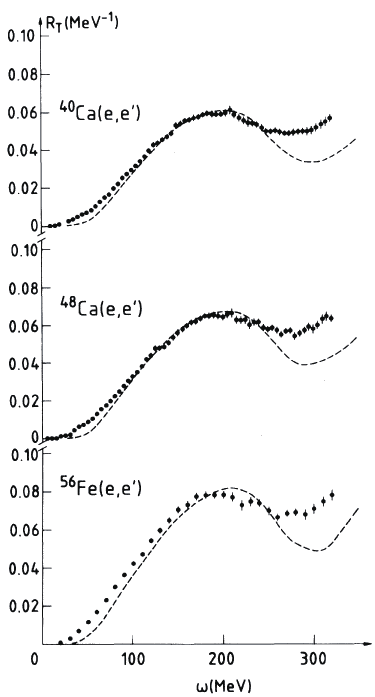
\includegraphics[width=.8\linewidth]{figs/R_T_q_550.png}
\label{fig:R_T_q_550}
\end{subfigure}
\caption[R LT q 550]{
(a) $R_L$ and (b) $R_T$ of $^{40}$Ca, $^{48}$Ca, and $^{56}$Fe at $|\vec{q}|$ = 550 MeV/c.
Description of curves are same as in Figure \ref{fig:R_LT_q_410}
\label{fig:R_LT_q_550}}
\end{figure}

The Coulomb Sum Rule is extracted from the data mentioned above with three momentum transfer in the range
200 MeV/c $\leq q \leq$ 550 MeV/c, by integrating $R_L$ over the experimental measured region of energy loss
$\omega$. As shown in Figure\ref{fig:S_L_data}, the light nuclei ($^{3}$He) reach unity at high $q$ quickly.
There is a clear sign of quenching from theoretical calculation up to 40\% for medium ($^{56}$Fe, $^{40}$Ca and
$^{48}$Ca) and heavy nuclei ($^{208}$Pb).

\begin{figure}[h]
\centering
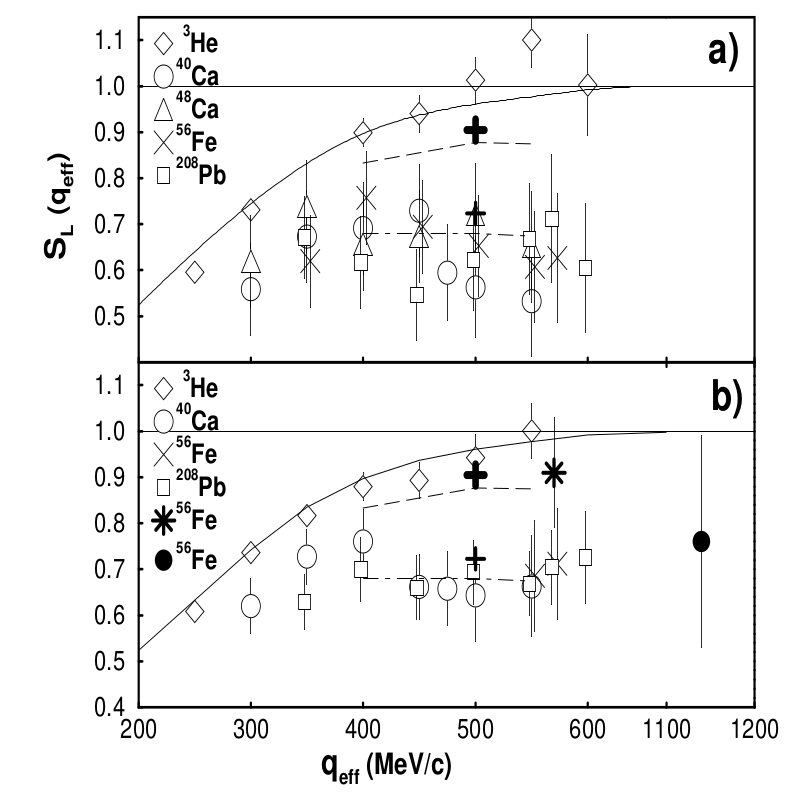
\includegraphics[width=0.7\textwidth]{figs/S_L_data.png}
\caption[S L data]{
5. Longitudinal (a) and transverse (b) response functions of $^{208}$Pb at
$q_{eff}$ = 550 MeV/c extracted in the EMA. Saclay data only (filled circles), combined with $^{197}$Au \SI{15}{\degree} SLAC data (triangles
up), combined with Bates $^{238}$U \SI{60}{\degree}
data (triangles down); previous Saclay results with Coulomb corrections [19]:
thin solid lines. c) Longitudinal response function at $q_{eff}$ = 500 MeV/c (same
experimental symbols). Nuclear matter calculations: dashed line, Hartree
Fock calculations including short range correlations and final state interactions with free nucleon form factors
(solid line), with modified nucleon
form factors (dotted-dashed line).
Figure reproduced from \cite{Meziani2001}.
\label{fig:S_L_data}}
\end{figure}


A later analysis on Saclay and SLAC data by Jourdan\cite{Jourdan1995} suggested that no quenching
exists by using the distorted wave Born approximation with the Coulomb corrections.
However, reanalysis of Saclay Data by Morgenstern and Meziani\cite{Meziani2001} with the effective
momentum approximation showed that quenching still exists. The comparison between
Morgenstern and Meziani's analysis and Jourdan's work is presented in Table \ref{tab:calc_compare}.
Two differences are identified: (a) the Coulomb corrections and (b) the use of the total error in
the Saclay data but only the statistical error in the SLAC data by Jourdan.

\begin{table}[tb!]
\begin{tabular}{ccccc}
\hline
Analysis & \begin{tabular}[c]{@{}c@{}}Saclay\\ Uncertainty\end{tabular} & \begin{tabular}[c]{@{}c@{}}SLAC\\
Uncertainty\end{tabular} & Coulomb Correction & $S_L$         \\ \hline
Jourdan  & total                                                        & statistical
& No                 & 0.86$\pm$0.12 \\
         & total                                                        & statistical
         & Yes                & 0.91$\pm$0.12 \\ \hline
         M\&M     & total                                                        & (*)
         & No                 & 0.72$\pm$0.23 \\
                  & total                                                        & (*)
                  & Yes                & 0.63$\pm$0.20 \\
                           & total                                                        & total
                           & No                 & 0.82$\pm$0.12 \\
& total                                                        & total
& Yes                & 0.73$\pm$0.12 \\ \hline
\end{tabular}
\label{tab:calc_compare}
\end{table}


\section{Theoretical Models}
Since the 1980s, great efforts have been made to resove the $R_L$ quenching problem (or the missing charge problem).
The traditional non-relativistic models cannot explain the problem.

Some models including relativistic corrections, final state interactions, and two-body and many body correlations.
These effects are important but not large enough to explain all the quenching of $R_L$ if the predicted $R_T$ is 
to remain in agreement with the experiment data.

In order to explain this puzzle , several more exotic explanations have been raised:

\begin{itemize}
\item Inadequate Coulomb correction:
The idea of the Rosenbluth separation of the longitudinal and transverse re-
sponse functions is based on the Plane Wave Born Approximation (PWBA)
and one photon exchange. This approximation is not valid for medium and heavy nuclei 
because the Coulomb field of the nucleus. In a large Z nucleus, the strong Coulomb field
of the nuclei will distort the wave front of the electron and modifies the electron scattering
cross section as well as the $R_L$ and $R_T$.
The effect of the Coulomb field can be calculated with the Distorted Wave Born Approximation (DWBA).
However, DWBA cross section cannot be written in a separable form, and are extremely time consuming in
numerical complications. Due to these difficulties, the Effective Momentum Approximation (EMA) is developed.
Inadequacy of the Coulomb corrections for the analysis of existing experiments
were thought to be the reason of quenching for medium and heavy nuclei.

\item Swollen nucleon models: Noble first suggested  another approach that there could be
an effective change in the size of the nucleon in the nuclear medium  ~\cite{Noble1981},
and this is also used to explain the EMC effect.
The changing of nucleon size in the nuclear medium may relate to the partial
deconfinement of quarks in the nuclear medium, which leads to a modified
quark distribution in the nucleus. 
Noble's calculations indicated a 30\% increase in the nucleon charge radius. He calculated the CSR by
using the Fermi gas model (FGM) with an increased charge radius. The results are
shown in Figure~\ref{fig:swollen}.

%\item The relativistic models which were based on hadron and meson degrees of freedom
%were used to calculate $R_L$. Although, the agreement between the calculations and the 
%experiments improved, the agreement is not good enough to explain the total quenching of
%$R_L$.
\end{itemize}

\begin{figure}[h]
\centering
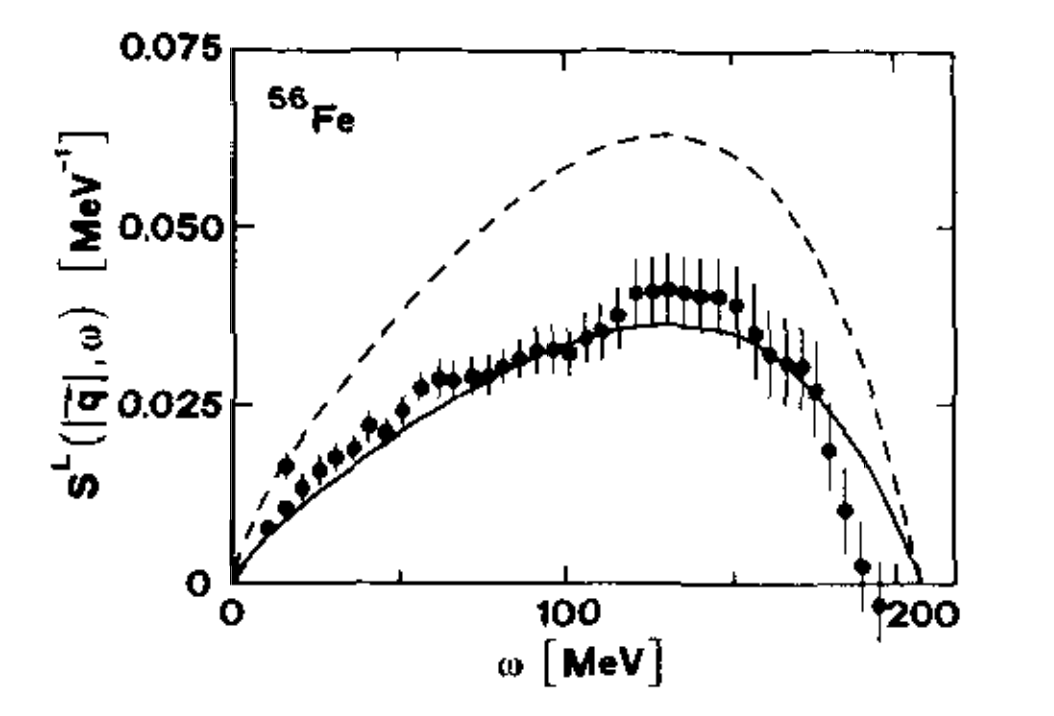
\includegraphics[width=0.7\textwidth]{figs/swollen.png}
\caption[swollen]{
Longitudinal structure function in the relativistic FGM calculation of Noble
\cite{Noble1981} for |q| = 410MeV/c($k_f$ = 1.11 fm$^{−1}$). Experimental data from Altemus \cite{Altemus1980}.
Broken curve: impulse aproximation; Full curve: results with scaled root mean square
radius.
Figure reproduced from \cite{Orlandini1991}.
\label{fig:swollen}}
\end{figure}

%\section{Experiment Kinematics}

\cite{*}

%%%%%%%%%%%%%%%%%%%%%%%%%%%%%%%%%%%%%%%%%%%%%%%%%%%%%%%%%%%%%%%%%%%%%%
% -*-latex-*-

% -*-latex-*-

%% This is an example first chapter.  You should put chapter/appendix that you
%% write into a separate file, and add a line \include{yourfilename} to
%% main.tex, where `yourfilename.tex' is the name of the chapter/appendix file.
%% You can process specific files by typing their names in at the
%% \files=
%% prompt when you run the file main.tex through LaTeX.

% Beamline: Beam Energy
% BCM : charge
% BPM & raster:  beam position
% HRS Magenets: HRS Central momentum
% Scintillator & Trigger: livetime

\chapter{Experiment Setup}
\label{Experiement_Setup}

During an experiment that ran from October 10th  2007 to January 16th 2008, in Hall A of Thomas Jefferson National
Accelerator Facility (Jefferson Lab), the Coulomb Sum Rule was tested. To determine Coulomb Sum Rule, both response function $R_L$ and $R_T$ of different nuclei (${}^1$H, ${}^4$He, ${}^{12}$C, ${}^{56}$Fe, ${}^{208}$Pb) have been measured from inclusive scattering in the quasi-elastic region. In this chapter, the experiment setup and most of instrumentations will be introduced briefly. 

\section{Overview}

During the CSR experiment, an unpolarized electron beam was scattered from ${}^4$He, ${}^{12}$C, ${}^{56}$Fe and
${}^{208}$Pb target to measure the cross-section in quasi-elastic region. The Hall A High Resolution Spectrometer (HRS)
was used to detect the scattered electrons at 4 different angles: \SI{15}{\degree}, \SI{60}{\degree}, \SI{90}{\degree} and \SI{120}{\degree}.
The relative big difference between scattering angles allowed for the largest Rosenbluth lever arm within a single experiment compared to all previous experiments.
The cross section data were used to extract the $R_L$ and $R_T$ response functions and Coulomb Sum Rule.

To have as much covarage as possible in ($q$, $\omega$) to reduce systematic uncertainties in the Rosenbluth interpolation procedure,
the data were acquired in beam energies between 400 MeV and 3679 MeV , spectrometer central momentum between 100 MeV/$c$ and
3.6 GeV/$c$, see Table.~\ref{tab:E_E'_table}. The kinematic coverage of the CSR experiment is shown in Figure.~\ref{fig:kinematic_coverage}.

\begin{table}[tb!]
\center
\begin{tabular}{|c|c|c|c|c|c|c|c|}
\hline
\multicolumn{2}{|c|}{\SI{15}{\degree}} & \multicolumn{2}{c|}{\SI{60}{\degree}} & \multicolumn{2}{c|}{\SI{90}{\degree}} & \multicolumn{2}{c|}{\SI{120}{\degree}} \\ \hline
$E$      & $E'_{low}$    & $E$     & $E'_{low}$    & $E$     & $E'_{low}$    & $E$     & $E'_{low}$     \\ \hline
1260     & 810           & 646     & 187           & 400     & 100           & 400     & 100            \\
1646     & 1147          & 740     & 250           & 528     & 108           & 528     & 98             \\
2145     & 1605          & 845     & 305           & 646     & 127           & 646     & 107            \\
2448     & 1838          & 957     & 377           & 740     & 170           & 740     & 110            \\
2845     & 2135          & 1030    & 270           & 845     & 135           & 845     & 105            \\
3249     & 2440          & 1102    & 333           & 957     & 267           & 957     & 237            \\
3679     & 2770          & 1260    & 370           & 1030    & 100           &         &                \\ \hline
\end{tabular}
\caption[E E' talbe]{Incident energy and the lowest scattered energy detected (in MeV) at each kinematics.} \label{tab:E_E'_table}
\end{table}

\begin{figure}[h]
\centering
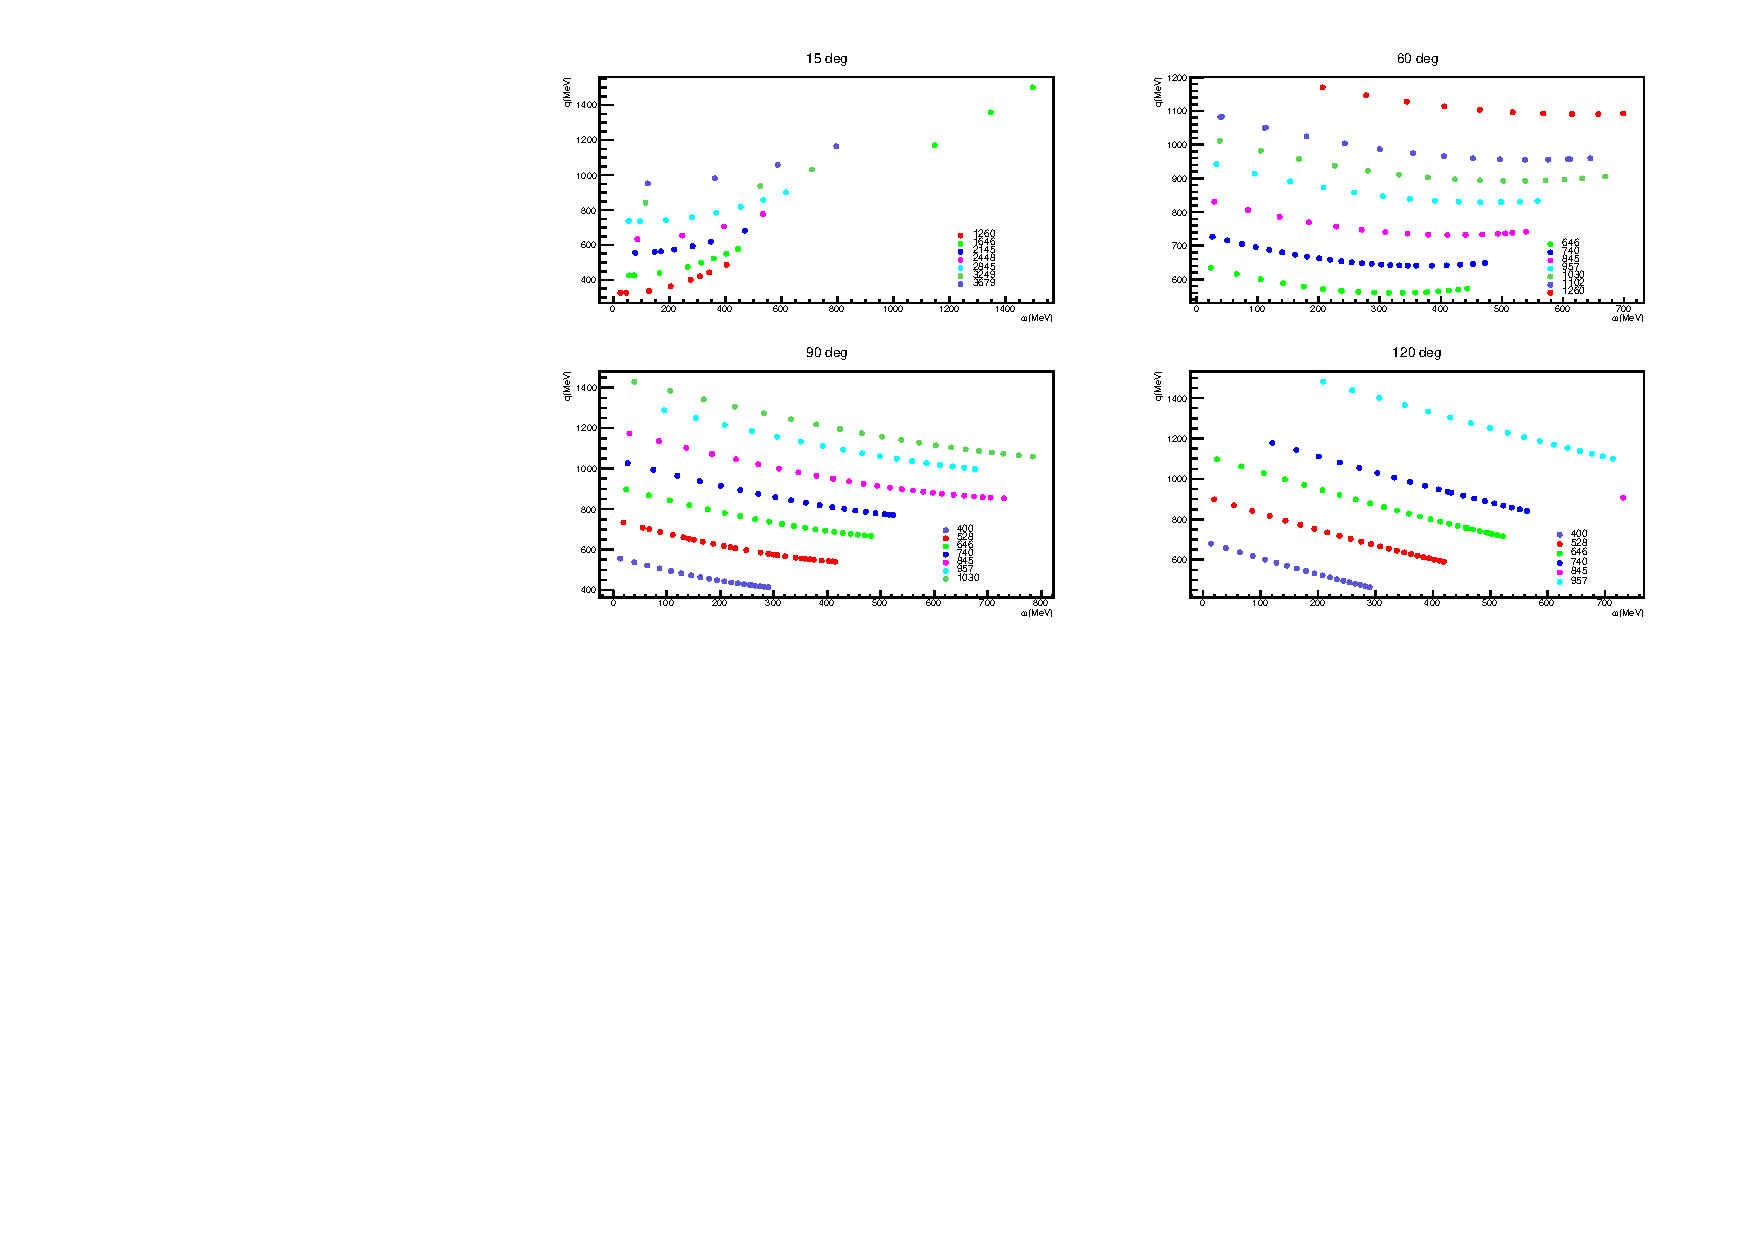
\includegraphics[width=0.7\textwidth]{figs/He4kinematics.pdf}
\caption[He4 kinematic]{Kinematic coverage of the CSR experiment. Each graph for a scattering angle, each color represent a beam energy.
The y axis is three momentum transfer (MeV) and the x axis is energy loss $\omega$ (MeV).
\label{fig:kinematic_coverage}}
\end{figure}

This chapter will discuss the electron beam, the Hall A beamline components, the cryogenic and solid targets and the HRS system.

\section{The Accelerator and Electron Beam}
The Continuous Electron Beam Accelerator Facility (CEBAF) at Jefferson Lab (JLab) was built to investigate the structure
of nuclei and hadrons and the underlying fundamental interactions in the region below the high-energy "asymptotically
free" regime. 

The accelerator consists of an electron injector, two super-conducting linear accelerators, recirculation arcs,
and RF separators. The layout of accelerator is shown in Figure.~\ref{fig:JLab_overview}.


\begin{figure}[h]
\centering
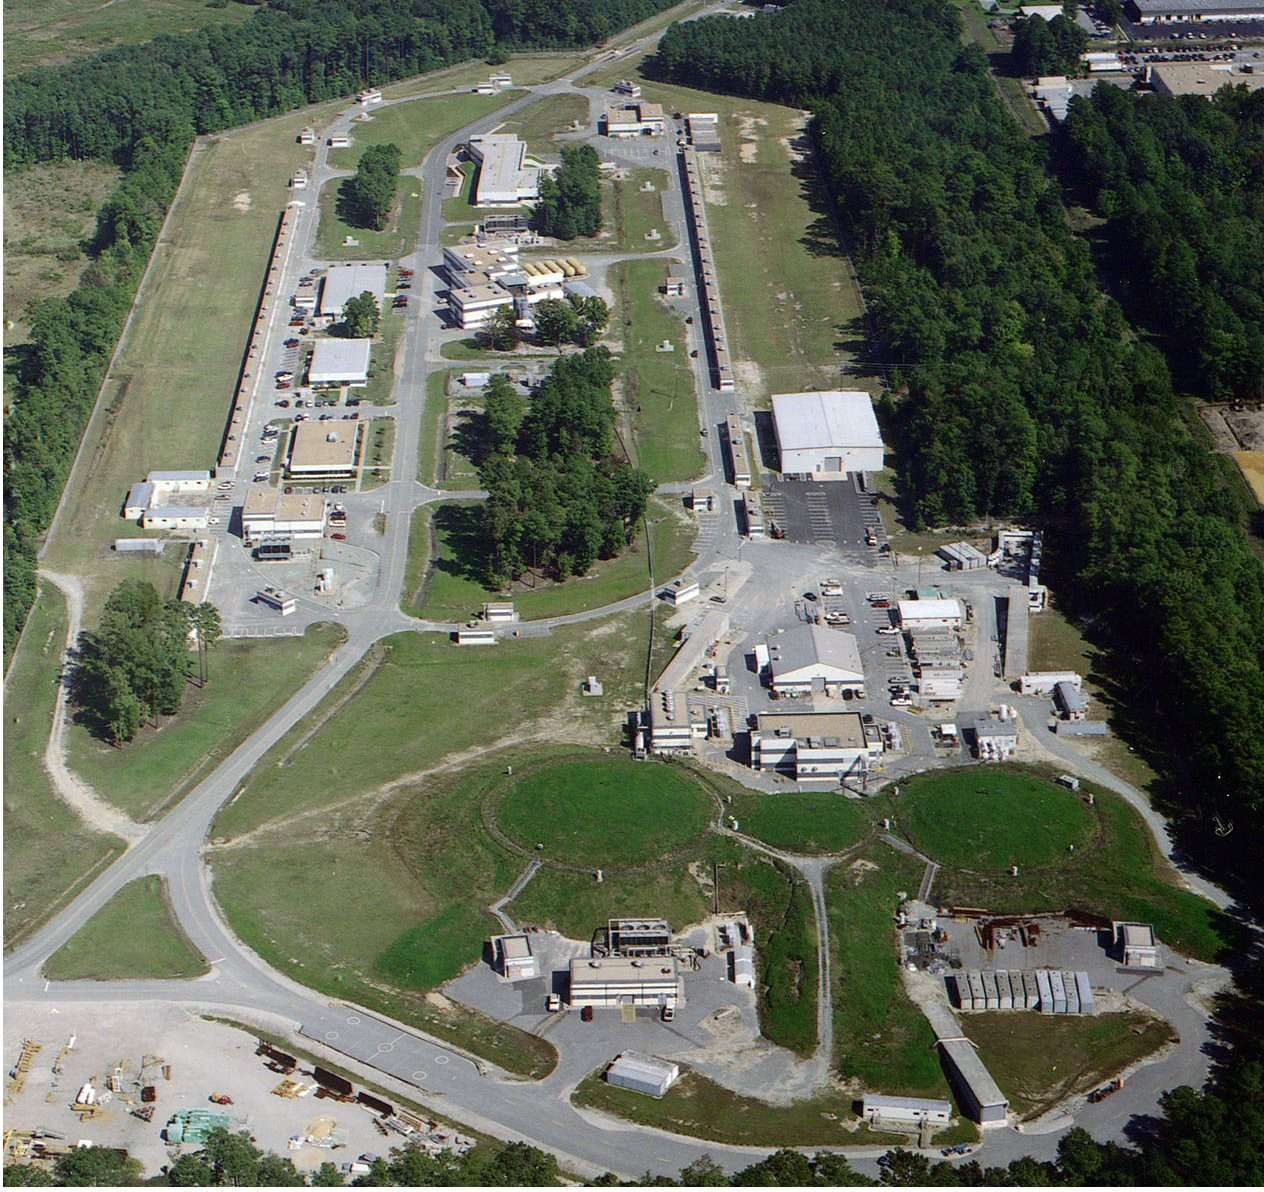
\includegraphics[width=0.7\textwidth]{figs/JLab_overview.png}
\caption[JLab overview]{JLab overview.  \label{fig:JLab_overview}}
\end{figure}

%injector
The source of polarization electrons is a strained GaAs cathode at injector. The cathode is illuminated by a 1497 MHz
gain-switched 780 nm diode laser.  It provides polarized beam of above 70\% polarization.

% linacs
The beam is first accelerated to 45 MeV in the injector, then is transported to the north linac. Each linac
contains 20 cryomodules (this was the situation before 12 GeV upgrade; 5 new cryomodules were added to each linac after the
upgrade). There are eight super-conducting niobium RF cavities in each cryomodule. The RF cavities are phased to provide
maximum acceleration. The nominal gain of each linac is 400 MeV, and it can be tuned up to 500 MeV, which made it possible to accelerate the beam up to 5.7 GeV.
Liquid Helium from the at CHL (Central Helium Liquefier) keeps the superconducting cavities at a temperature of 2 K.

%arcs
The north and the south linacs are connected by recirculation arcs with radius 80 m that can turn the beam by
\SI{180}{\degree} from the south to the north linac and vice versa, forming a recycling beamline in the shape
of a "racetrack". Each arc has more than 2,200 quadruple or dipole magnets to provide the field that keeps the beam on a precise
path and tightly focused.

After passing through the south linac, the beam can either go to the next recirculation arc for another pass around the accelerator, or enter one of the
experiment halls using RF extraction. The designed maximum current is 200 $\mu$A, which can be split arbitrarily to
three 499 MHz bunch trains, one for each hall.  The CSR experiment required 50 $\mu$A average current, with energies ranging from 0.4 to 4 GeV.


\section{Beam Energy Measurement}
There beam energy measurement is an important part of the experiment to ensure the accuracy. There are two independent
methods to measure the absolute beam energy :  Arc measurement, which is based on measurements of the beam deflection in
a known field; and eP measurement, which is based on measurement of the electron elastic scattering off carbon target.  
During the CSR experiment, only the Arc measurement was used.

%% Measurement principle; uncertainty; 
\subsection{Arc Measurement}
The principle of this method is that electrons in a magnetic field will move in circular patten, with the radius
depending on field strength and electron's momentum. The Arc method measures the bending radius of the beam in the
arc section, see Figure.~\ref{fig:arc-measurement}. 

\begin{figure}[tb!]
\centering
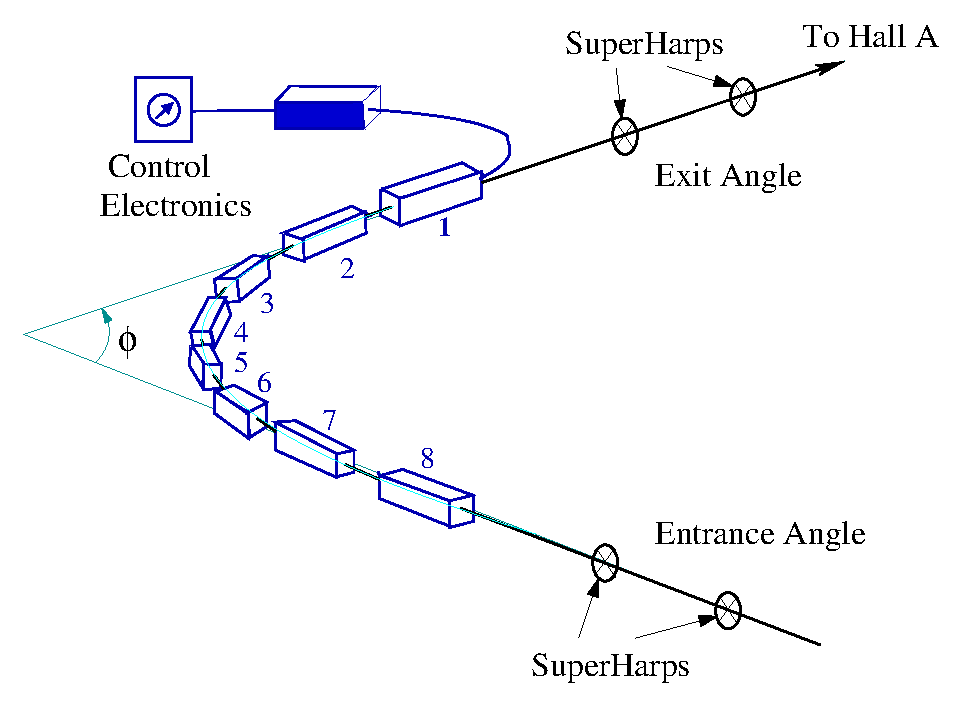
\includegraphics[width=0.8\textwidth]{figs/arc-measurement.pdf}
\caption[Arc Measurement]{Arc section of Hall A beamline.  \label{fig:arc-measurement}}
\end{figure}

The momentum of the beam ($p$ in GeV/c) is then related to the field integral in eight dipoles ($\int\vec{B}\times\partial\vec{l}$
in T$\cdot$ m) and the net bending angle through the arc section ($\theta$ in radians) by:
\begin{equation}
  P = k \frac{\int\vec{B}\times\partial\vec{l}}{\theta}
\end{equation}

where $k=0.299792$ GeV $\cdot$ rad $\cdot$ T$^{-1}$ $\cdot$ m $^{-1}$. 

Detailed description of the Arc measurement can be found in \cite{Alcorn2004}.
The arc measurement consists of two simultaneous measurements. One is for the bending angle of the beam measured by a set of wire scanners. Another is for the field strength integral $\int\vec{B}\times\partial\vec{l}$ of the eight dipoles based on the reference magnet(9 th dipole) field measurement.
There are two operation modes in the arc section: the dipersive (invasive) and non-dispersive(non-invasive) mode. The
dispersive mode will affect the quality of the beam, but has better precision ($\Delta E_{beam}/E_{beam} = 2\times10^{-4}$) than non-dispersive mode ($5\times10^{-4}$).

The Arc measurement during the CSR experiment is done at a beam energy of 845 MeV. The measurement result ($845.08 \pm
0.2$ MeV) is consistent with the so-called "Tiefenbach" energy ($844.87 \pm 0.4$ MeV), calculated from the Hall A arc
$\vec{B}\partial\vec{l}$ value and the Hall A beam position measured from the beam position monitor(BPM). 

%The uncertainty of the Arc measurement is at $2\times10^{-4}$ level.

%\section{Hall A Overview}
%The Hall A has a diameter of 53 m. The basic layout of Hall A is shown in figure below. It basically can be divided into three parts: the beamline appratus (BPM, BCM, Raster, Moller, Compton, etc), target system, the left and right HRS spectrometers(??).

%\begin{figure}
%\centering
%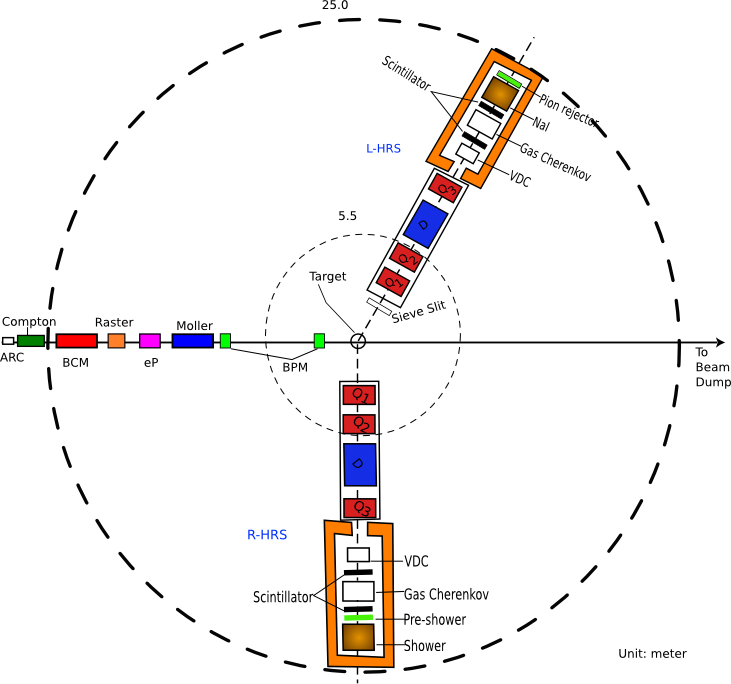
\includegraphics[width=\textwidth]{figs/Hall_A_overview.png}
%\caption[Hall A Overview]{Hall A Overview.  \label{Hall_A_overview}}
%\end{figure}


\section{Beam Charge Measurement}
The incident number of beam electrons is an essential normalization factor in the extraction of cross sections.
It is proportional to the beam current measured by the Beam Current Monitor (BCM) in Hall A,
which provides a stable, low-noise, non-interfering beam current measurement \cite{Alcorn2004}.

The BCM consists of an Unser monitor, two RF cavities, associated electronics and a data-acquisition system.
The diagram of BCM is shown in Figure.~\ref{fig:BCM_diagram}.
The cavities and the Unser monitor are located 25 m upstream of the target.
The Unser monitor is a parametric current monitor which provides an absolute reference.  
The two resonant FR cavity monitors on two sides on the Unser Monitor are stainless steel
cylindrical high-Q ($~$ 3000) waveguides which are tuned to the frequency of the beam (1.497 GHz)
resulting in voltage levels at their outputs being proportional to the beam current.
Each of the RF output signals from the two cavities is split into sampled and integrated parts.

\begin{figure}[tb!]
\centering
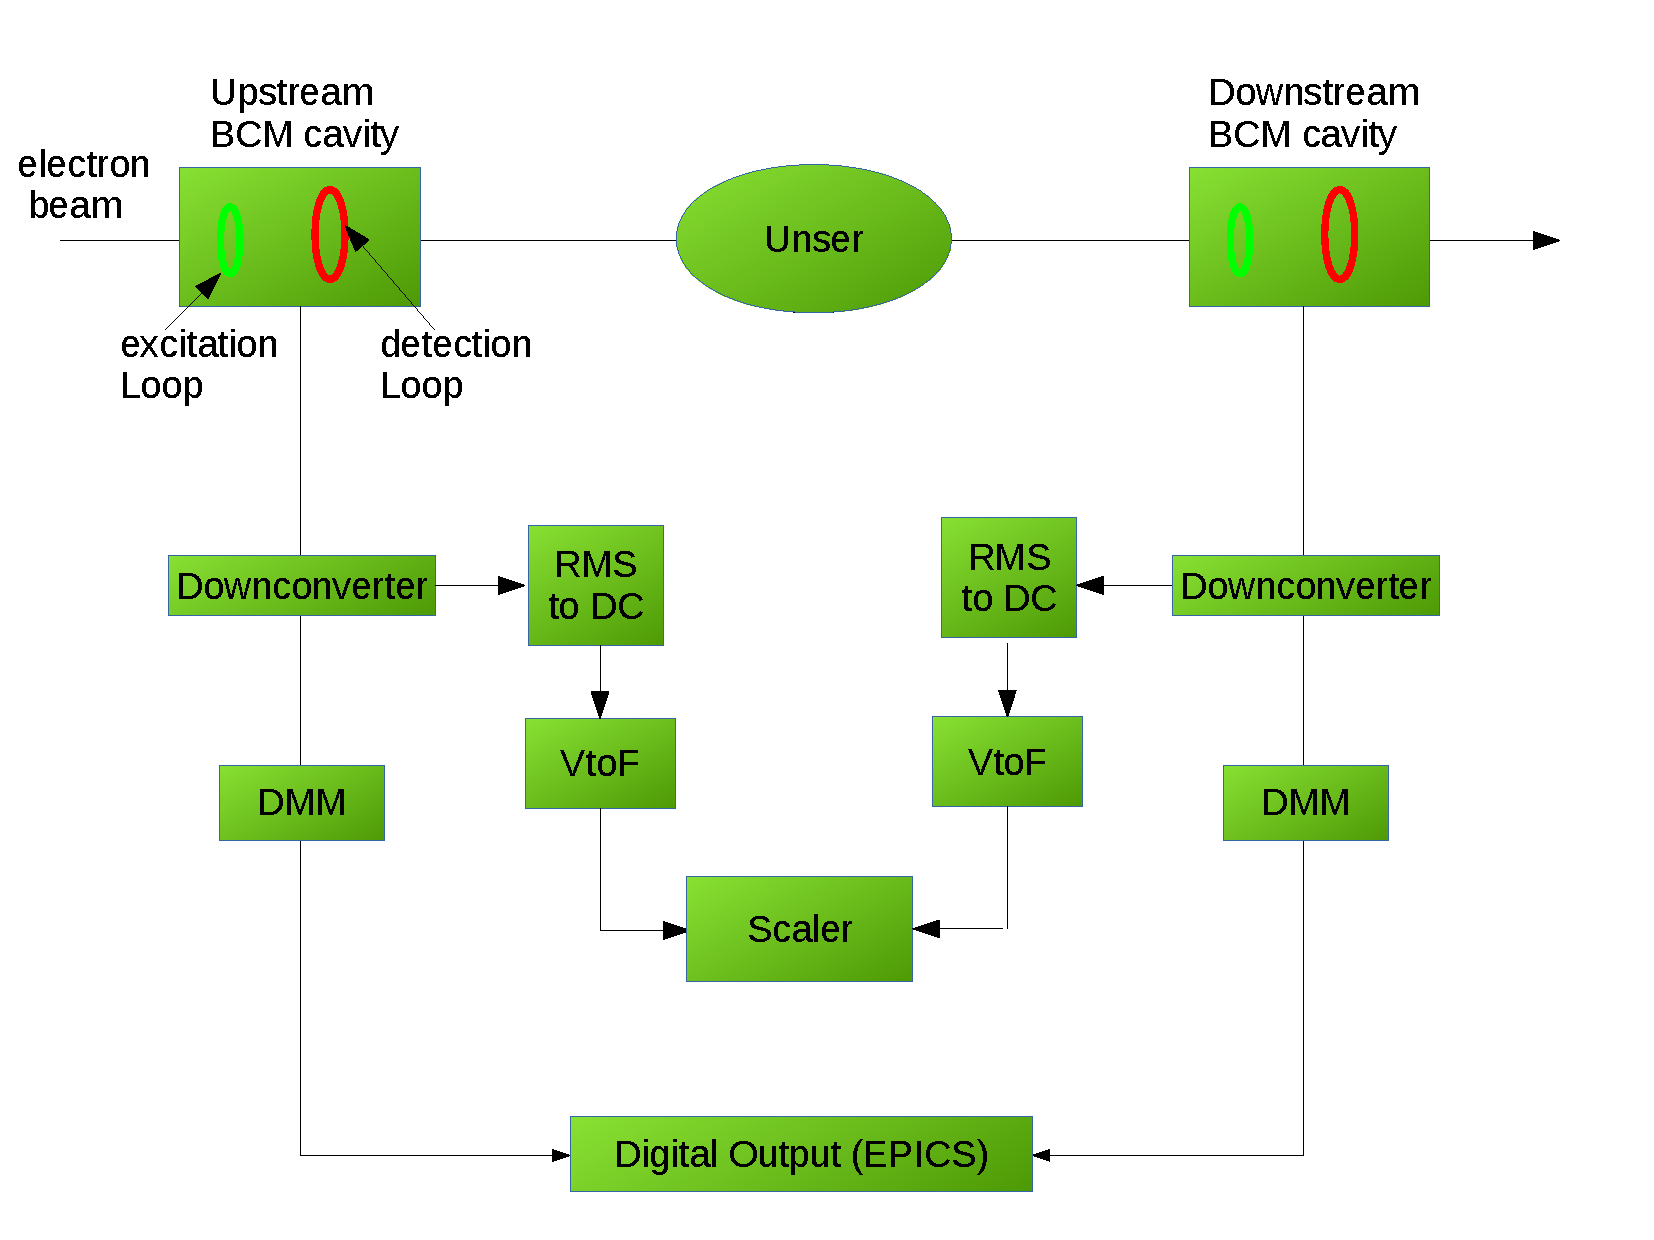
\includegraphics[width=0.8\textwidth]{figs/BCM_diagram.pdf}
\caption[BCM diagram]{Beam current monitor diagram. Plot reproduced from \cite{Alcorn2004}.   \label{fig:BCM_diagram}}
\end{figure}


The sampled data is sent to a high-precision Digital Multi-Meter (DMM),
which provides an output signal representing the RMS of the input signal
during that second. The output is proportional to the beam charge accumulated
for that second. The signals from both cavities are sent to a computer
through GPIB cables, and are recorded every 1-2 s in the EPICS 
(Experimental Physics and Industrial Control System) database.

The integrated data is sent to an RMS-to-DC converter to generate
an analog DC voltage level. The voltage level is sent to 
a Voltage-To-Frequency(VtoF) converter whose output frequency is
proportional to the input.
The frequency signal is fed to 200 MHz VME scalers and stored in
stream with other scaler information every 4 seconds.
The scaler value accumulates during the run and is proportional
to the time-integrated voltage level.
The regular RMS to DC output is linear for currents from 5$\mu A$ to
200 $\mu A$. A set of amplifiers with different gain factors ($\times$ 1,
$\times$ 3, $\times$ 10) can extend the linear region to lower currents.
%So there are three signals from each RF cavity (U1, U3, U10 or D1, D3 D10). 
The six signals for each spectrometer (U1, U3, U10 and D1, D3, D10, corresponding to the 3 gain factors and the up and
downstream cavities respectively) are sent to scalers and provide
the charge information during a run with redundancy.

The beam charge can be derived from BCM scaler reading as
\begin{equation}
Q_{bcm \times n} (\mu C) = \frac{\frac{Scaler_{bcm \times n}}{T} -Offset_{bcm \times n}}{Constant_{bcm \times n}} T
\end{equation}
where n=1, 3, 10 is the gain factor of the amplifiers, $T$ is the clock time for each run (in seconds),
Scaler$_{bcm \times n}$ is the BCM scaler reading for each gain factor.
The Offset$_{bcm \times n}$ and Constant$_{bcm \times n}$ are calibrated in BCM calibrations during CSR experiment, and are
given in Table ~\ref{tab:BCM_calibration}.

%The BCM calibration during CSR experiment gave the values of scaler calibration constants and offsets of upstream and
%downstream cavities, which are listed in Table .\ref{tab:BCM_calibration}.

\begin{table}[tb!]
\centering
\begin{tabular}{|c|c|c|c|c|}
\hline
Gain & \begin{tabular}[c]{@{}c@{}}Upstream\\ Calibration Constants\end{tabular} & \begin{tabular}[c]{@{}c@{}}Upstream\\
Offsets\end{tabular} & \begin{tabular}[c]{@{}c@{}}Downstream\\ Calibration Constants\end{tabular} &
\begin{tabular}[c]{@{}c@{}}Downstream\\ Offsets\end{tabular} \\ \hline
1    & 2372.38                                                                  & 362.5
& 24727.91                                                                   & 160.1
\\ \hline
3    & 7294.51                                                                  & 350.2
& 7517.37                                                                    & 126.7
\\ \hline
10   & 22067.11                                                                 & 442.6
& 23485.15                                                                   & 321.1
\\ \hline
\end{tabular}
\caption[BCM calibration]{BCM calibration constants and offsets.} \label{tab:BCM_calibration}
\end{table}

\section{Beam Position Monitor and Raster}
The beam typically has a Gaussian distribution across the cross-sectional area with full width at half maximum (FWHM)
$\sigma \approx$ 100 $\mu$m. To avoid damaging the target, the beam is rastered to a few millimeters in size. 
The raster is a pair of horizontal (X) and vertical (Y) air-core dipoles located 23 m upstream of the target.
There are two modes of the raster: sinusoidal and amplitude modulated.
In the sinusoidal mode, both X and Y dipoles are driven at 18 kHz with a \SI{90}{\degree} phase difference
which produces a circular pattern. The radius of the circular pattern is controlled by a function generator.
In the CSR experiment, a 2 mm $\times$ 2 mm sinusoidal mode was used on both the cryogenic targets and solid targets.

The beam position is an important parameter for the optics calibration and acceptance calculation of the spectrometers.
Two Beam Position Monitors located at 7.524 m and 1.286 m upstream of the target are used to determine the 
 position and direction of the beam at the target. 
Each BPM consists of four wire antennas parallel to the beam direction, which are tuned to the beam RF frequency 1.497 GHz.
They are placed symmetrically around the beam pipe in a vacuum chamber.
When a electron passes through the BPM, it will induce signals in antennas.
The amplitude of signal in each antenna is reverse by proportional to the distance between the antenna and the beam.
%So the beam position can be extracted in the BPM local coordinates.

The absolute position of the BPMs can be calibrated with respect to the harps near each of the BPMs.
The beam position information are stored in two ways:

\begin{enumerate}
\item The average beam position data over a 0.3 s time period are recorded in EPICS database and injected asynchronously
into the data stream
every 3-4 s.
\item The event-by-event beam position information is recorded in the CODA data stream from each of the 8 BPM antennas (2
$\times$ 4), and are also recorded in the data stream.
\end{enumerate}

The beam position and direction can be reconstructed from BPM information $x_{bpma,b}$ and $y_{bpma,b}$ as:

\begin{equation}
x_{beam} = \frac{x_{bpma} \cdot z_{bpmb} - x_{bpmb} \cdot z_{bpma}}{z_{bpmb}-z_{bpma}}
\end{equation}

\begin{equation}
y_{beam} = \frac{y_{bpma} \cdot z_{bpmb} - y_{bpmb} \cdot z_{bpma}}{z_{bpmb}-z_{bpma}}
\end{equation}

\begin{equation}
\theta_{beam} = \frac{x_{bpmb} - x_{bpma} }{z_{bpmb}-z_{bpma}}
\end{equation}

\begin{equation}
\phi_{beam} = \frac{y_{bpmb} - y_{bpma} }{\sqrt{(x_{bpmb} - x_{bpma})^2+(z_{bpmb}-z_{bpma})^2 }}
\end{equation}
where $z_{bpma}$ = -7.345 m, $z_{bpmb}$ = -2.214 m.  


% target structure
% solid target, liquid target (LH, LHe)

\section{Target System}

\subsection{Target Chamber}
The standard target vacuum chamber is used in the CSR experiment (see Figure.~\ref{fig:target_chamber}). The vacuum chamber is constructed out of several 1037-mm diameter rings, supported on a 607-mm diameter central pivot post. 
The stainless-steel base ring has one vacuum pump-out port and other ports for viewing and electrical feed-throughs. The
middle ring is made out of aluminum and located at the beam
height with 152-mm vertical cutouts on each side of the beam over the full angular range (that can accommodate
scattering angles within \SI{12.5}{\degree} $\leq$ $\theta$
$\leq$\SI{167.5}{\degree}). The cutouts are covered with
a pair of flanges with thin (0.38 mm) aluminum foils. It also has entrance and exit beam ports. The upper ring is used to house the cryotarget.

\begin{figure}[tb!]
\centering
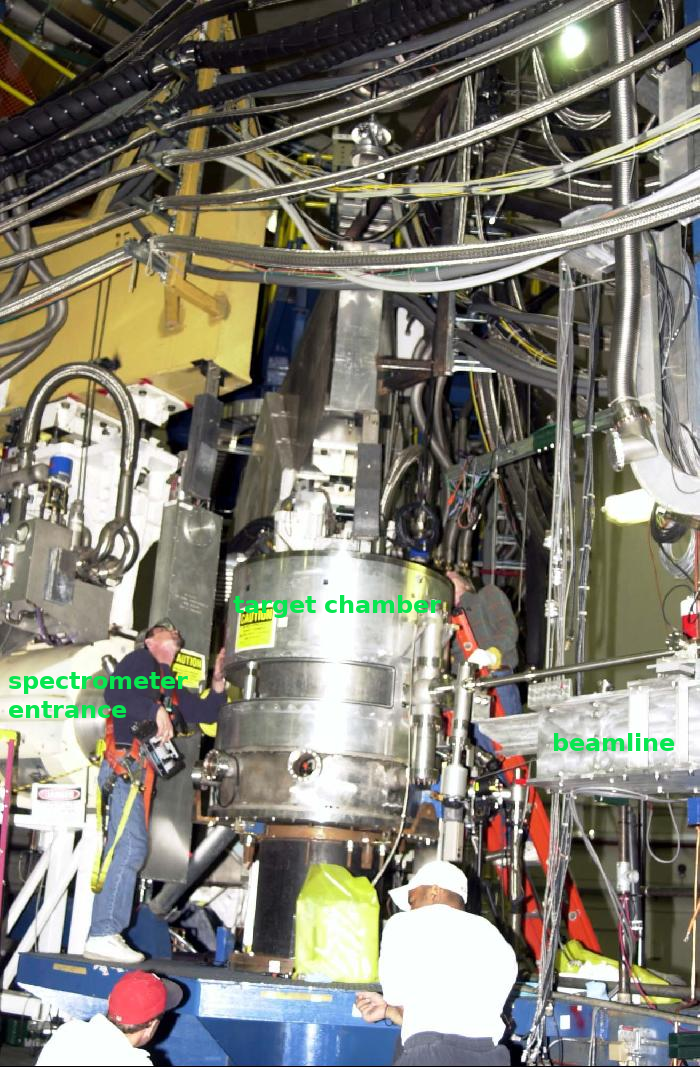
\includegraphics[width=0.6\textwidth]{figs/target_chamber_word.png}
\caption[Hall A target chamber]{Hall A target chamber.  \label{fig:target_chamber}}
\end{figure}

\subsection{Target Configuration of CSR}
The CSR experiment used targets from light nuclei to heavy nuclei in order to study medium dependency of 
Coulomb Sum rule.
Several targets: $^{2}$H, $^{4}$He, $^{12}$C, $^{23}$Al, Empty, BeO, $^{56}$Fe and $^{208}$Pb --- were used in this experiment.
These targets were installed on a target ladder in the target chamber and can be controlled remotely.


The position of the target ladder is vertical in the path of the electron beam.
The target system is controlled by three servo motors, each connected to its own motion controller called a BDS.
Two of  the BDS units are configured as "Slaves" and are controlled by the third, the "Master".
The target operator moves the target with the Master BDS through IOCs(input-output controllers) during the
experiment.
The various target positions are stored as 15 encoder values on the control computer (IOC). An encoder that is attached to
the Master's servo motor determines the target BDS position. The target positions are listed in Table~\ref{tab:tgmat-BDS}.

\begin{table}[tb!]
\centering
\begin{tabular}{lrr}
\hline
Target            & Material         & BDS Position \\ \hline
Loop 1 10cm       & High Pressure He & 32932800     \\
Loop 2 15 cm + Pb & He + Pb          & 26954176     \\
Loop 2 10 cm      & He               & 23377856     \\ \hline
Loop 3 15 cm + Pb & H$_2$ + Pb       & 19802560     \\
Loop 3 10 cm      & H$_2$            & 16241600     \\ \hline
Optics            & 7 carbon foils   & 12760000     \\
10 cm dummy       & 2 Al foils       & 10092480     \\
15 cm dummy       & 2 Al foils       & 9370560      \\
Empty             & N/A              & 8653760      \\
BeO               & BeO              & 6406480      \\
Beam right carbon & Carbon           & 4321550      \\
Beam right iron   & Iron             & 2692366      \\
Beam left carbon  & Carbon           & 585998       \\
Beam left iron    & Iron             & -1040625     \\ \hline
\end{tabular}
\caption[Target Materials and BDS Position.]{Target Materials and BDS Position for CSR experiment.}\label{tab:tgmat-BDS}
\end{table}

%cryogenic target
The cryogenic targets are mounted on the top layer of target ladder inside the target chamber with sub-system for cooling,
gas handling, temperature and pressure monitoring. 
The cryogenic target has three independent target loops, one gaseous helium loop (Loop 1) and two liquid hydrogen (LH2)
loops (Loop 2 and 3).

The Loop 1 target is a vertical "racetrack" shape cell, it is 10 cm long and 2cm wide. (See Figure.~\ref{fig:loop1})

\begin{figure}[tb!]
\centering
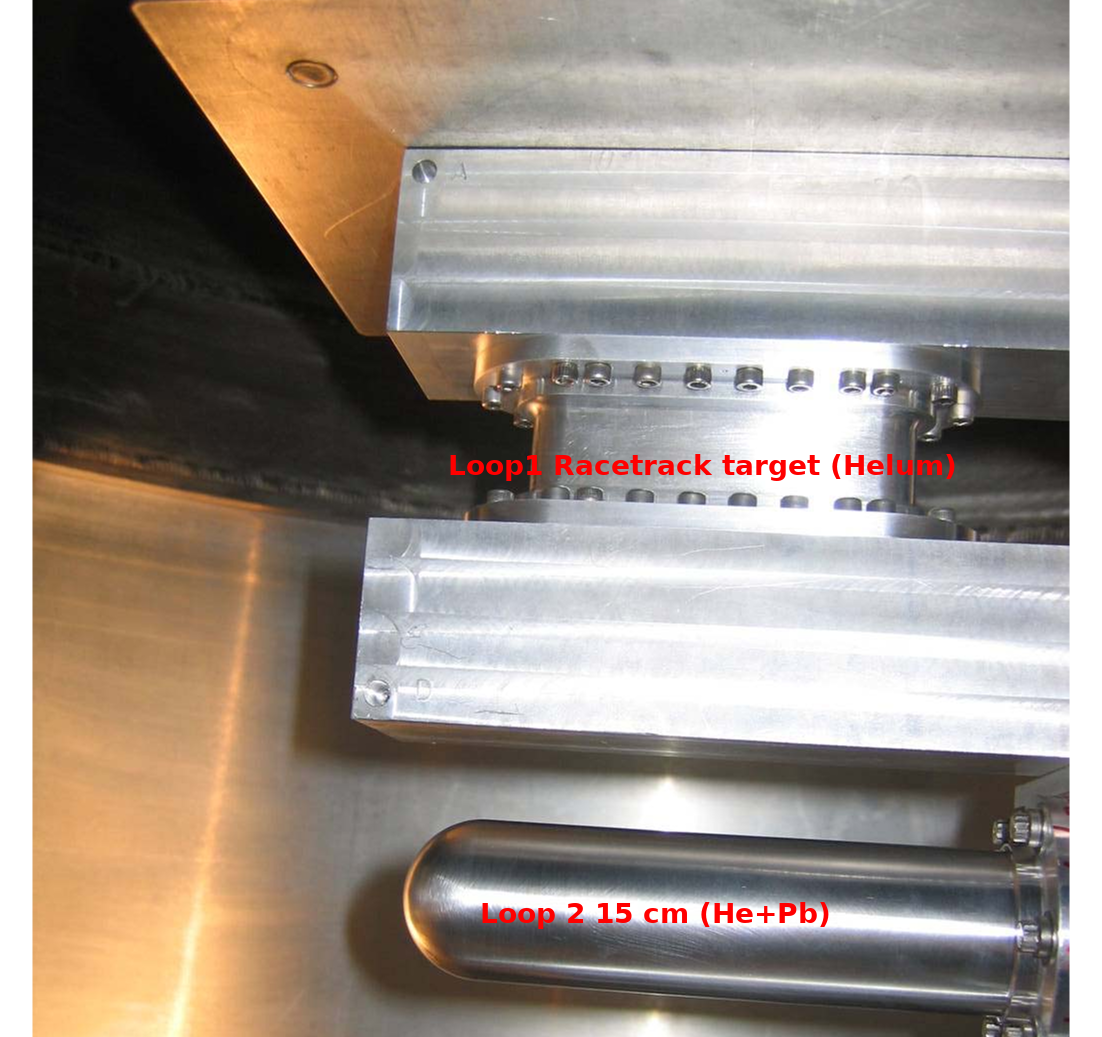
\includegraphics[width=0.8\textwidth]{figs/Loop1_target_edit.png}
\caption[Loop 1 cryogenic target ]{Loop 1 cryogenic target ($^4$He) }\label{fig:loop1}
\end{figure}

Loop 2 has two aluminum cylindrical target cells filled with Helium.
%comment: the 2 cells of Loop 2 both filled with Helium.
The upper cell is 15 cm long with a $^{208}$Pb foil held at the center
and tilted 50.0 $\pm$ \SI{2.00}{\degree} to the beam right, for cooling purpose.  The lower cell is 10 cm long filled
with $^{4}$He only.
Similarly, Loop 3 has 2 aluminum cylindrical target cells, both 15 cm long. The upper cell has a $^{208}$ Pb foil at
the center, also tilted 50.0 $\pm$ \SI{2.00}{\degree} to the beam right.
The lower cell is 15 cm long filled with liquid hydrogen only.
Loop 2 and Loop 3 cryogenic targets are shown in Figure.\ref{fig:loop2_loop3}.
Table.\ref{tab:window_thickness} gives the cell window and lead target thickness.

\begin{table}[tb!]
\centering
\scriptsize
\begin{tabular}{|l|l|l|r|l|l|}
\hline
Cryogenic Target & \begin{tabular}[c]{@{}l@{}}Entrance Window\\ (mm) $\pm$ 0.005\end{tabular} &
\begin{tabular}[c]{@{}l@{}}Exit Window\\ (mm) $\pm$ 0.005\end{tabular} & \begin{tabular}[c]{@{}r@{}}Lead thickness\\
($g/cm^2$)\end{tabular} & Beam left wall (mm) & Beam right wall (mm) \\ \hline
Loop1 10 cm      & 0.263 $\pm$ 0.008                                                          & 0.280 $\pm$ 0.005
& N/A                                                                 & 0.245 $\pm$ 0.002   & 0.239 $\pm$ 0.007    \\
\hline
Loop2 15 cm      & 0.128 $\pm$ 0.002                                                          & 0.194 $\pm$ 0.009
& 0.1057 $\pm$ 0.0001                                                 & 0.194 $\pm$ 0.009   & 0.194 $\pm$ 0.009    \\
\hline
Loop2 10 cm      & 0.257 $\pm$ 0.005                                                          & 0.120 $\pm$ 0.070
& N/A                                                                 & 0.120 $\pm$ 0.070   & 0.120 $\pm$ 0.070    \\
\hline
Loop3 15 cm      & 0.129 $\pm$ 0.001                                                          & 0.207 $\pm$ 0.005
& 0.3187 $\pm$ 0.0004                                                 & 0.207 $\pm$ 0.005   & 0.207 $\pm$ 0.005    \\
\hline
Loop3 15 cm      & 0.217 $\pm$ 0.003                                                          & 0.115 $\pm$ 0.001
& N/A                                                                 & 0.115 $\pm$ 0.001   & 0.115 $\pm$ 0.001    \\
\hline
\end{tabular}
\caption[Cryotargets window and lead target thicknesses]{Cryotargets window and lead target
thicknesses.}\label{tab:window_thickness}
\end{table}

The $^{4}$He gas target was operated at 7.0 K and about 170 psi, with a density about 0.12 g/cc. 
The nominal operating conditions of liquid targets are: 6.3 K at 1.4 MPa for $^{4}$He in Loop 2, 
and 19.0 K at 0.17 MPa for $^{2}$H in Loop 3.
The targets are cooled with helium supplied by the ESR (End Station Refrigerator).
The uncertainty in the target density is minimized by monitoring the pressure and temperature with pressure transducers.

\begin{figure}[tb!]
\centering
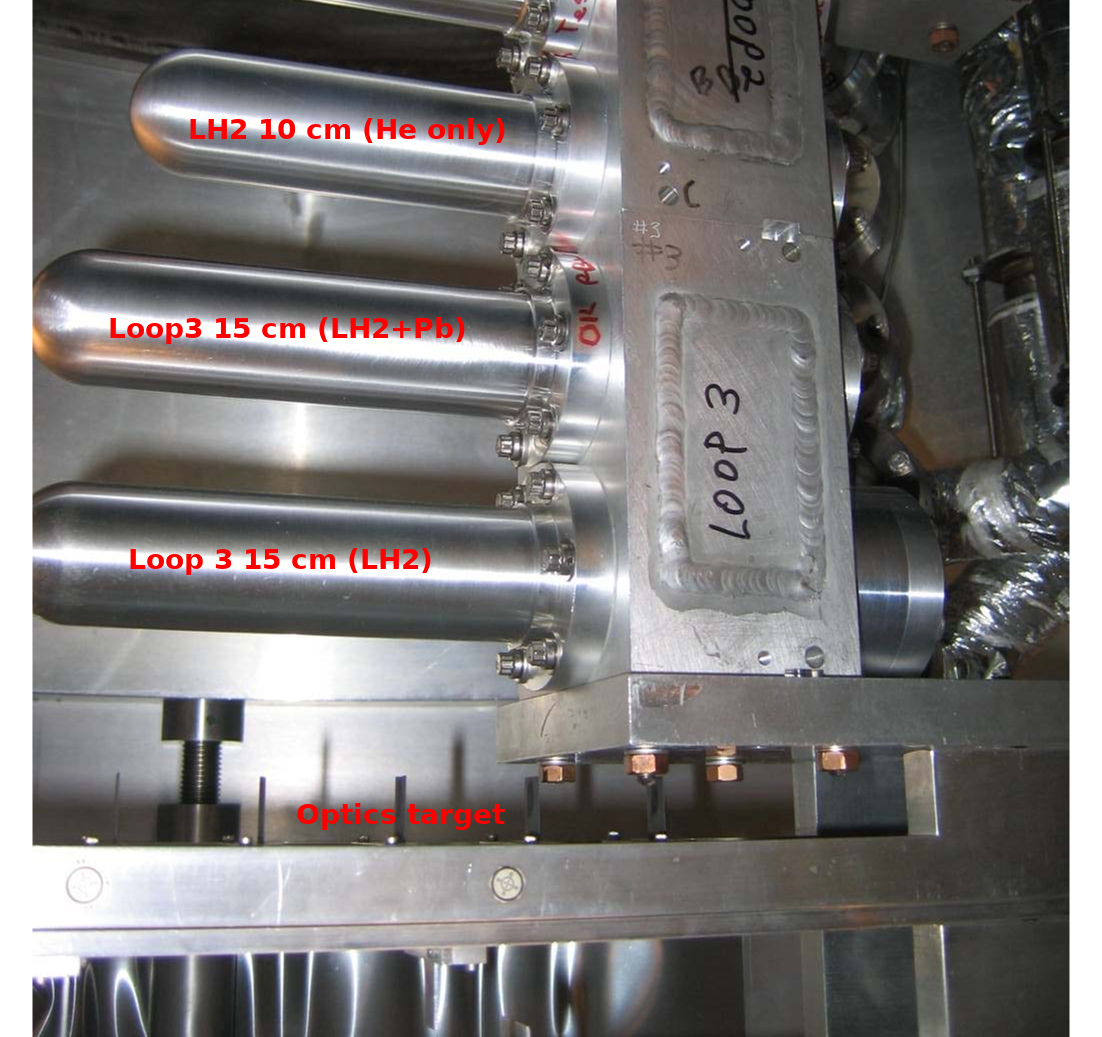
\includegraphics[width=0.8\textwidth]{figs/Loop2_Loop3_target_edit.png}
\caption[Loop 2 and Loop 3 cryogenic target ]{Loop 2 and Loop 3 cryogenic target. }\label{fig:loop2_loop3}
\end{figure}

%solid target

Next in the ladder are optics, dummy and empty targets (see Figure.\ref{fig:optics_dummy}).
The optics target are 7 carbon foils cut from the same 99.5\% chemically pure carbon sheet.
The thickness of each foil is 0.042 $\pm$ 0.001 g/cm$^2$, they are separated by 4 cm along the beam $\hat{z}$ direction.

\begin{figure}[tb!]
\centering
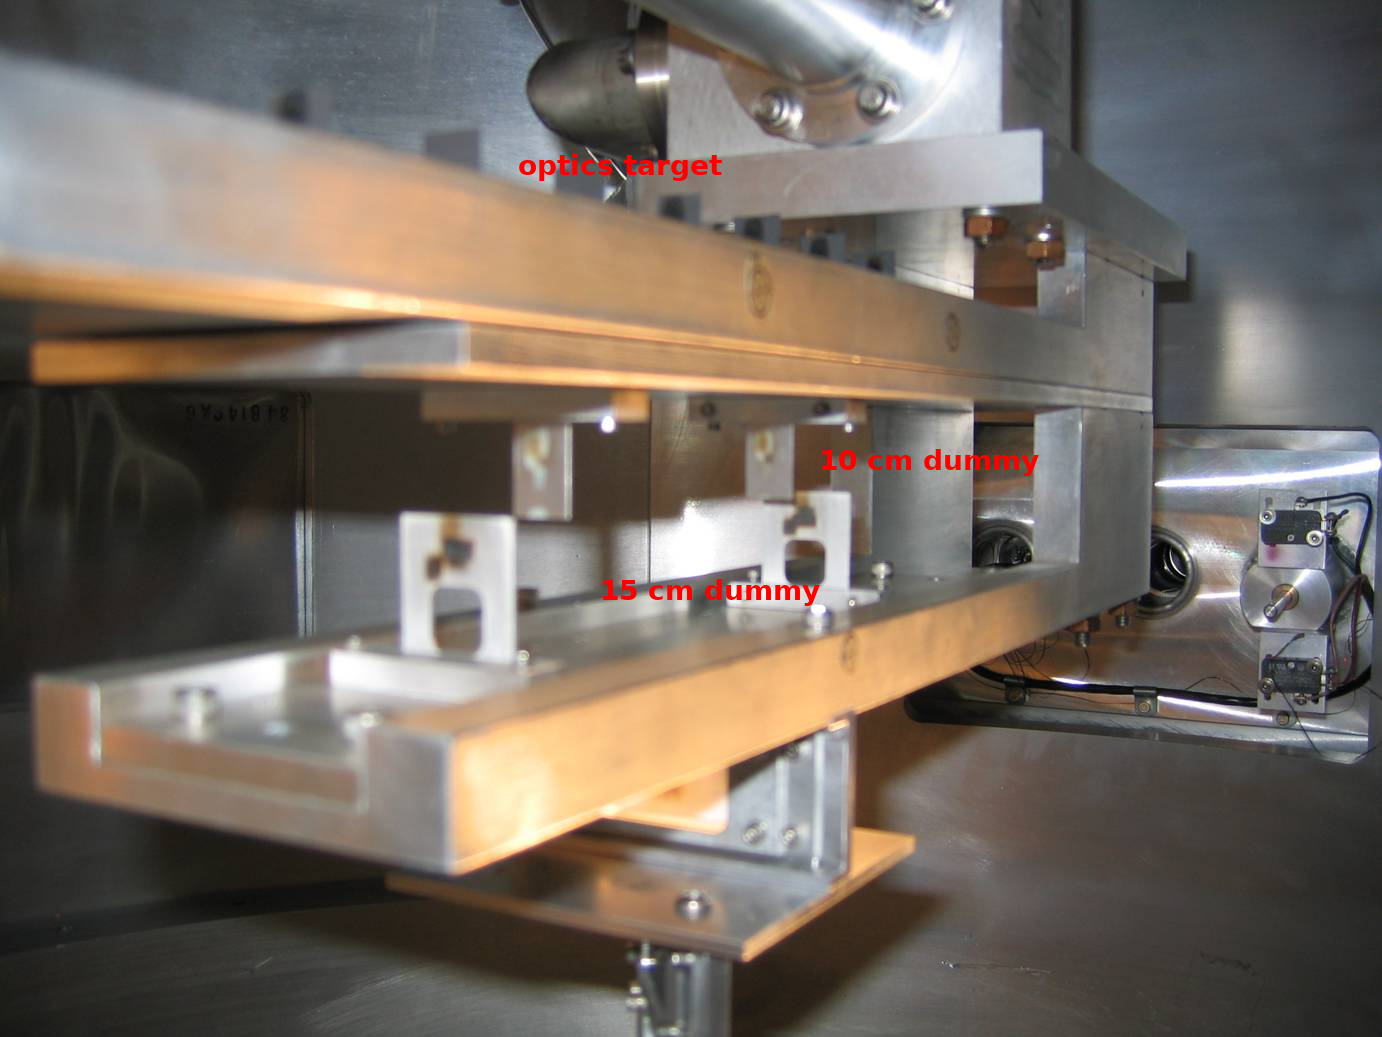
\includegraphics[width=0.8\textwidth]{figs/optics_dummy_target_edit.png}
\caption[Optics, dummy and empty target ]{Optics, dummy and empty target. }\label{fig:optics_dummy}
\end{figure}

The dummy targets are two pairs of aluminum foils with thickness 0.259 $\pm$ 0.001 g/cm$^2$.
One pair are separated by 10 cm in $\hat{z}$ direction (called "10 cm dummy target"), and another pair are separated by
15 cm in $\hat{z}$ direction (called "15 cm dummy target"), to measure the contribution from the window
of cryogenic targets.  There is a hole on each foil of the second dummy target, which is called "empty target".

The last on the target ladder are solid targets.
The upper position is for BeO which is perpendicular to the beam.
The second two positions are for carbon and iron targets and they are tilted \SI{51.78}{\degree}
clockwise when viewed from top, so the beam hits the right side of foils.
The bottom two positions are also for carbon and iron targets, but tilted \SI{48.56}{\degree}
counterclockwise, and the beam hit the foils from the left side. The configuration of the left and right titled solid
target are shown in Figure ~\ref{fig:left_right_tilted_target}.
%This design makes the electrons travel different length in target after scattering before
%they enter one or the other spectrometer. Therefore, by comparing the spectra from both HRSs,
%we can study the external radiative effect.
The solid targets are shown in Figure.\ref{fig:carbon_iron}.

\begin{figure}[tb!]
\centering
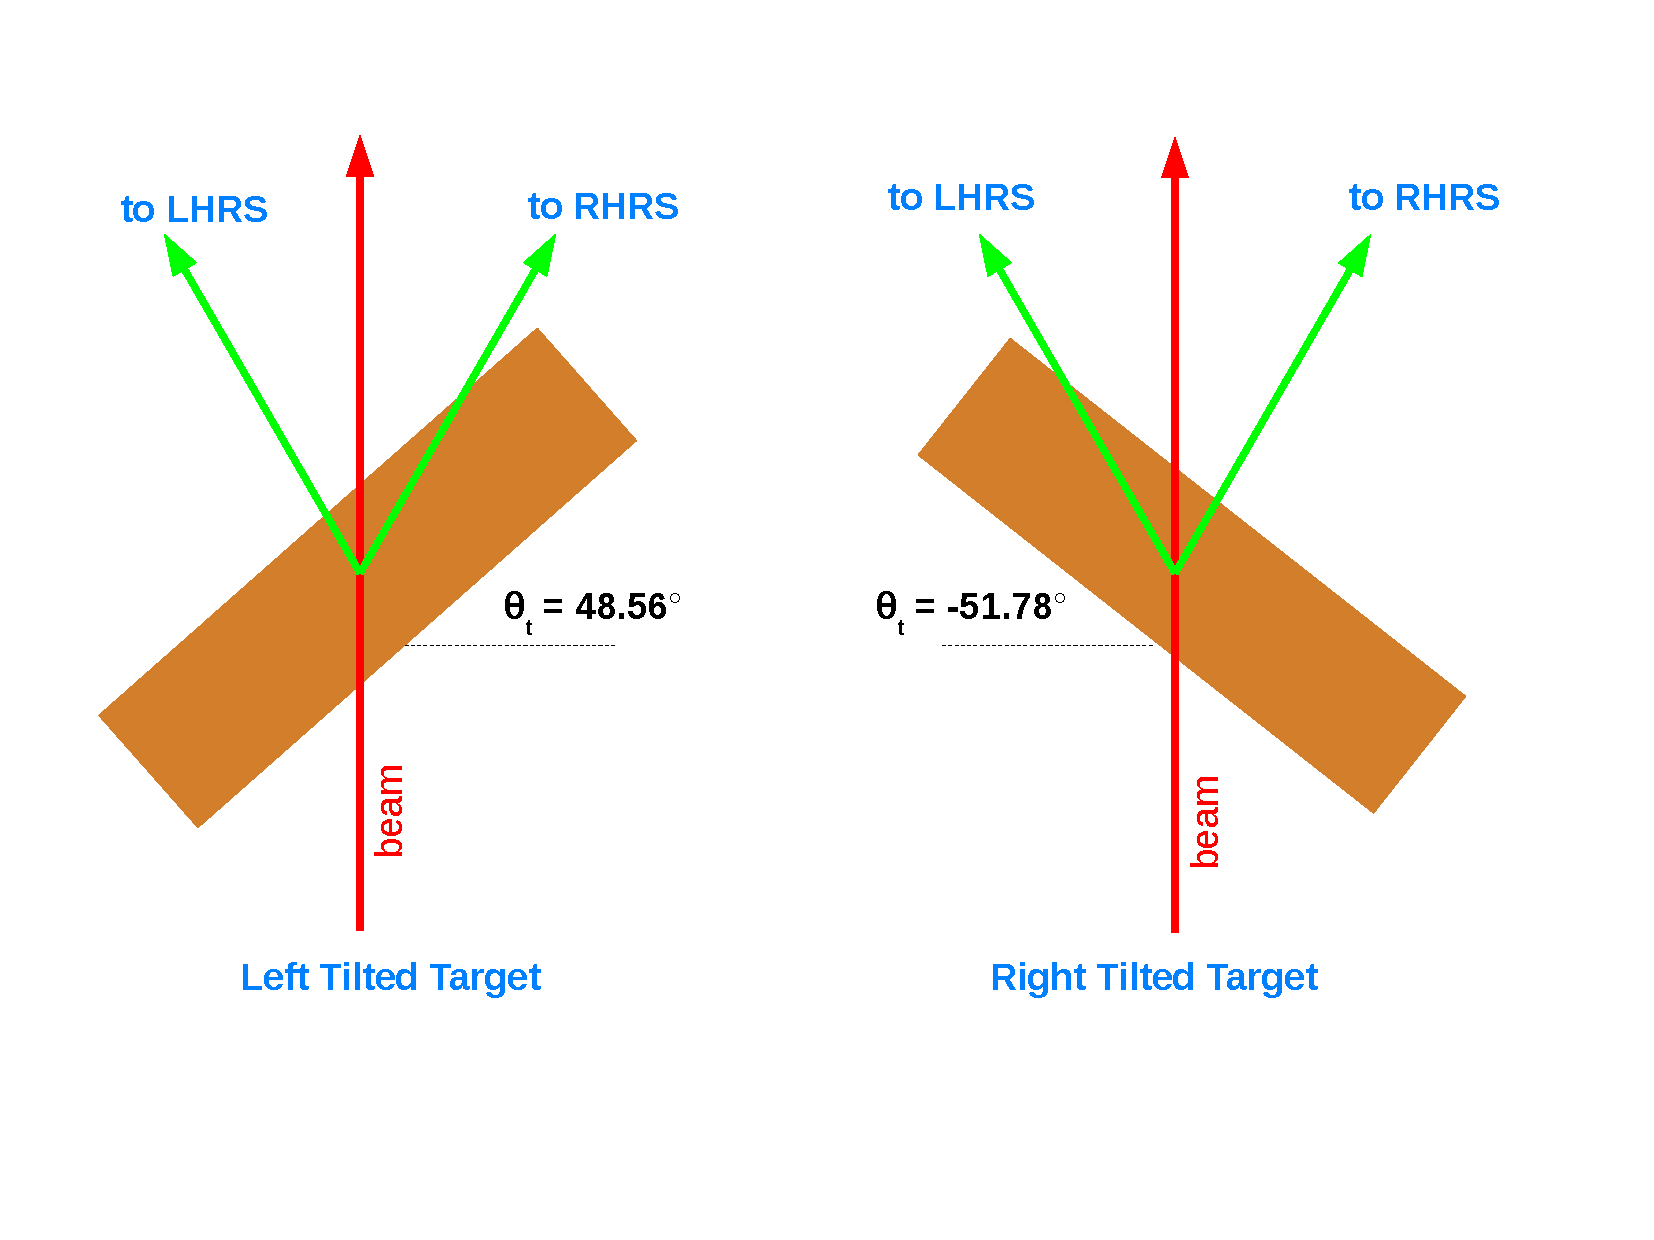
\includegraphics[width=0.8\textwidth]{figs/left_right_tilted_target.pdf}
\caption[left right tilted target ]{Configuration of left and right tilted target(viewed from the top). }\label{fig:left_right_tilted_target}
\end{figure}

\begin{figure}[tb!]
\centering
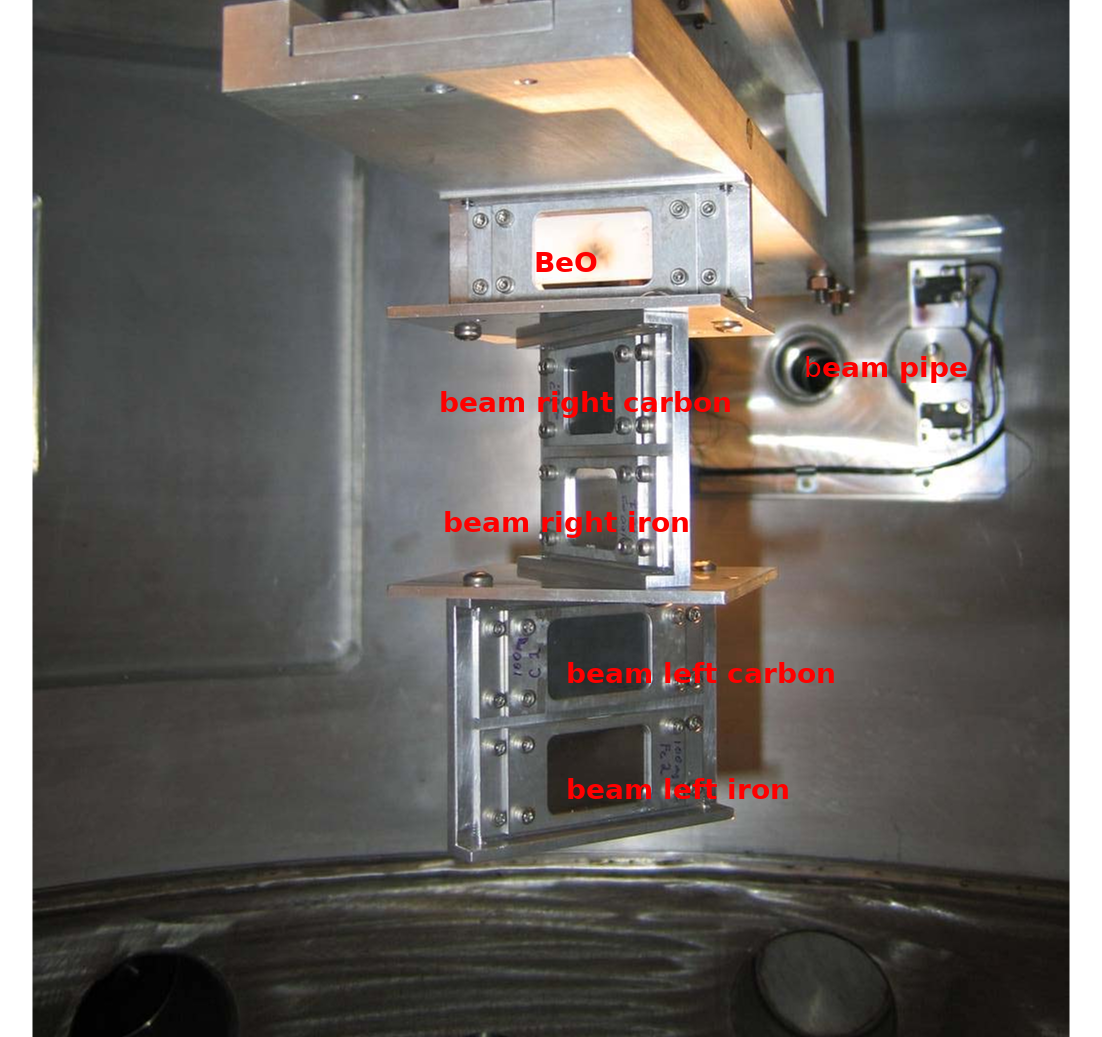
\includegraphics[width=0.8\textwidth]{figs/carbon_iron_target_edit.png}
\caption[Solid targets ]{Solid targets. }\label{fig:carbon_iron}
\end{figure}

Table.\ref{tab:purity_thickness} gives the target foil positions, thicknesses and chemical purities.

\begin{table}[tb!]
\centering
\begin{tabular}{|l|r|r|r|}
\hline
Purity  & Target Position   & Material & Thickness ($g/cm^2$) \\ \hline
99\%    & BeO               & BeO      & 0.149 $\pm$ 0.001    \\ \hline
99.95\% & Beam right carbon & Carbon   & 0.0894 $\pm$ 0.0001  \\ \hline
99.99\% & Beam right iron   & Iron     & 0.1027 $\pm$ 0.0001  \\ \hline
99.95\% & Beam left carbon  & Carbon   & 0.0895 $\pm$ 0.0001  \\ \hline
99.99\% & Beam left iron    & Iron     & 0.1023 $\pm$ 0.0001  \\ \hline
\end{tabular}
\caption[Solid target purity and thickness]{Solid target purity and thickness}\label{tab:purity_thickness}
\end{table}


\section{Hall A High-Resolution Spectrometers}
The core of the Hall A equipment is a pair of nearly identical spectrometers that can reach a maximum momentum bend of
4 GeV/$c$. These spectrometers were
designed to study electromagnetic interactions and hadronic structure with high precision.
Their basic layout is shown in Fig~\ref{fig:HRS_spectrometer}.
Important design characteristics of spectrometer are shown in the Table~\ref{tab:HRS_chars}.



\begin{figure}[tb!]
\centering
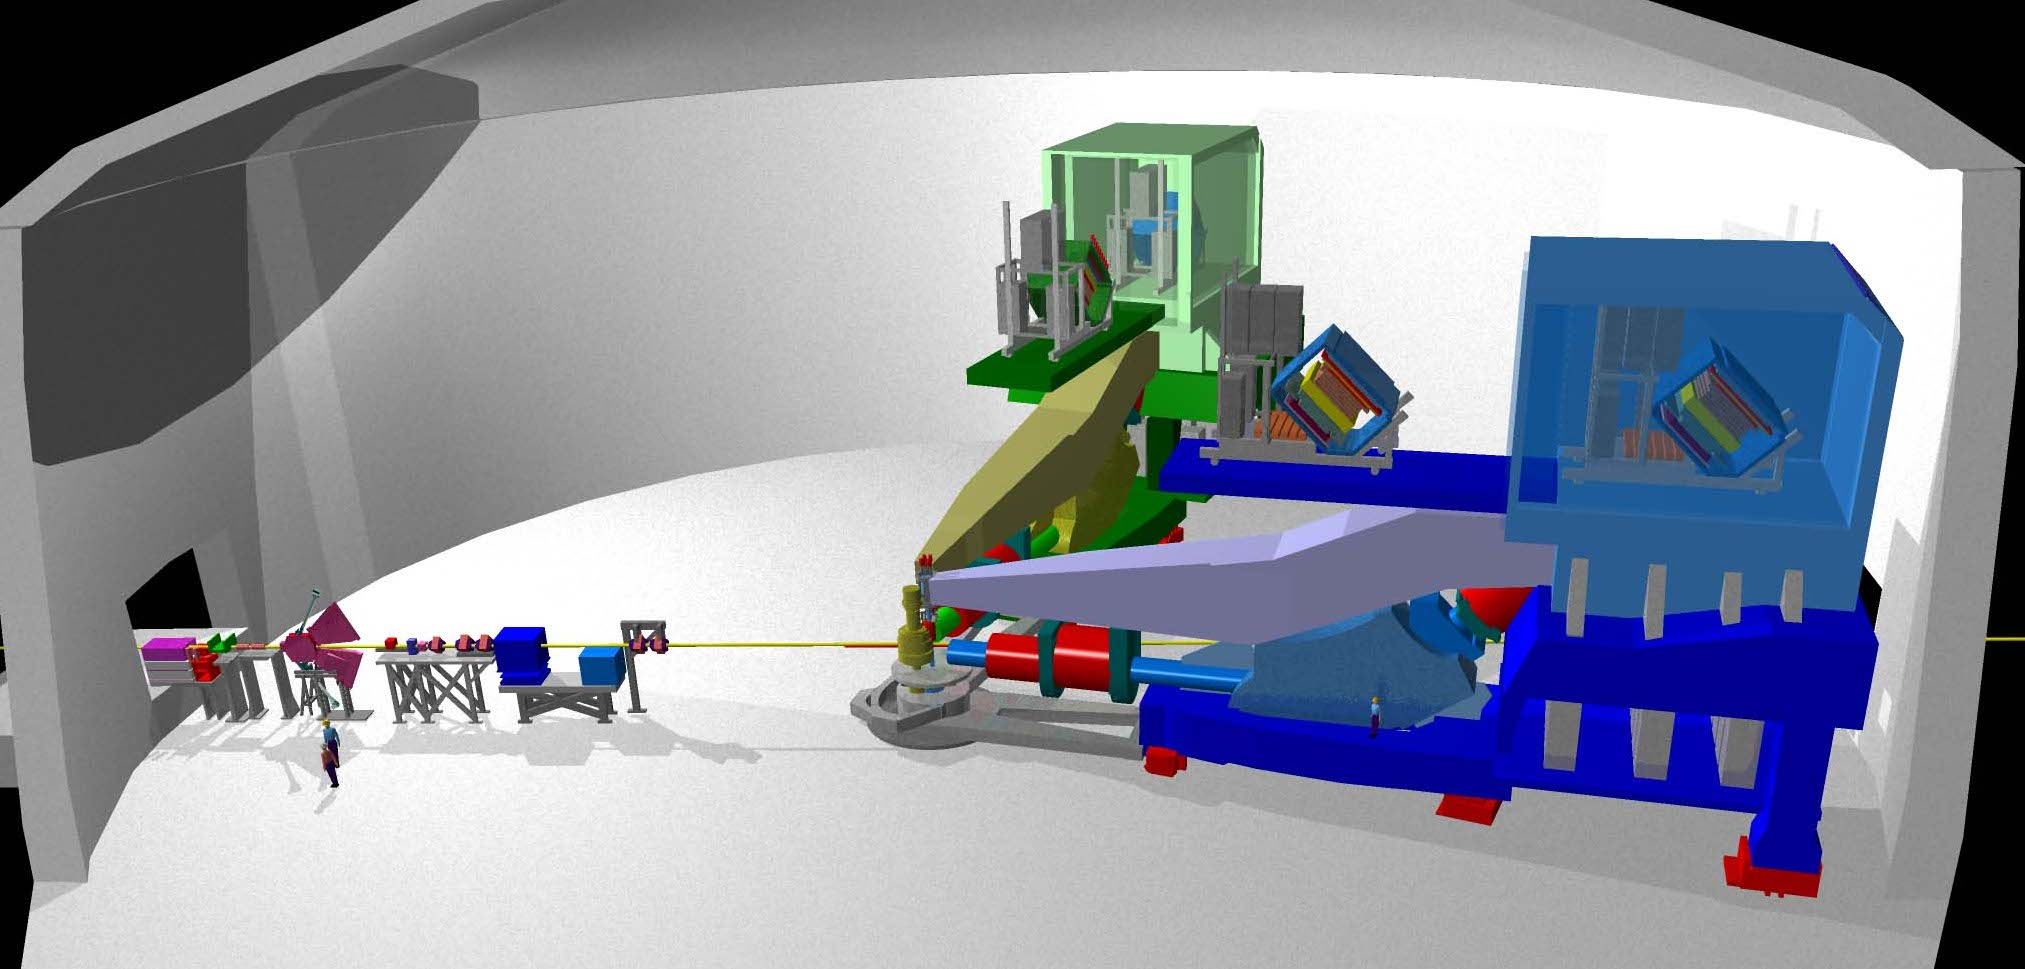
\includegraphics[width=0.9\textwidth]{figs/HRS_spectrometer.png}
\caption[Hall A HRS spectrometer]{The Hall A high resolution spectrometers.  \label{fig:HRS_spectrometer}}
\end{figure}

\begin{table}[tb!]
\begin{tabular}{ll}
\hline
Configuration                         & QQDQ vertical bend                  \\
Bending angle                         & \SI{45}{\degree}                    \\
Optical length                        & 23.4 m                              \\
Momentum range                        & 0.1 - 4.0 GeV/$c$                   \\
Momentum acceptance                   & -4.5 \% $<$ $\delta$p/p $<$ +4.5 \% \\
Momentum resolution                   & 1 $\times$ 10$^{-4}$                \\
Dispersion at the focus (D)           & 12.4 m                              \\
Radial linear magnification (M)       & -2.5                                \\
D/M                                   & 5.0                                 \\
Angular range                         &                                     \\
HRS-L                                 & 12.5 - \SI{150}{\degree}            \\
HRS-R                                 & 12.5 - \SI{130}{\degree}            \\
Angular acceptance                    &                                     \\
Horizontal ($\phi$)                   & $\pm$ 30 mrad                       \\
Vertical ($\theta$)                   & $\pm$ 60 mrad                       \\
Angular resolution                    &                                     \\
Horizontal ($\Delta\phi/\phi$)        & 0.5 mrad                            \\
Vertical ($\Delta\theta/\theta$)      & 1.0 mrad                            \\
Solid angle at $\delta$p/p=0, $y_0$=0 & 6 msr                               \\
Transverse length acceptance          & $\pm$ 5 cm                          \\
Transverse position resolution        & 1 mm                                \\ \hline
\end{tabular}
\caption[Main design characteristics of the Hall A high resolution spectrometers]
{Main design characteristics of the Hall A high resolution spectrometers.}\label{tab:HRS_chars}
Table reproduced from \cite{Alcorn2004}.
\end{table}


\subsection{Design and Characteristics of the Magnets}
Each HRS spectrometer has four superconducting magnets: three quadruples and one dipole.
The QQDQ magnet configuration (see Figure~\ref{fig:QQDQ_config}) (Q stands for quadruple and D stands for dipole) is used for a few requirements:
a high momentum resolution at the 10$^{-4}$ level over the 0.8 to 4.0 GeV/$c$ momentum range, a large acceptance
in both angle and momentum, good position and angular resolution in the scattering plane, and extended target
acceptance \cite{Alcorn2004}.
The first two quadruples are used to focus the scattered electrons vertically and horizontally, respectively,
to achieve the desired angular acceptance and avoid particles to collide with the magnets.
The dipole is mainly used to bend the electron trajectory \SI{45}{\degree} upward and to achieve a good
momentum resolution. The third quadruple will further focus beam horizontally. 

\begin{figure}[tb!]
\centering
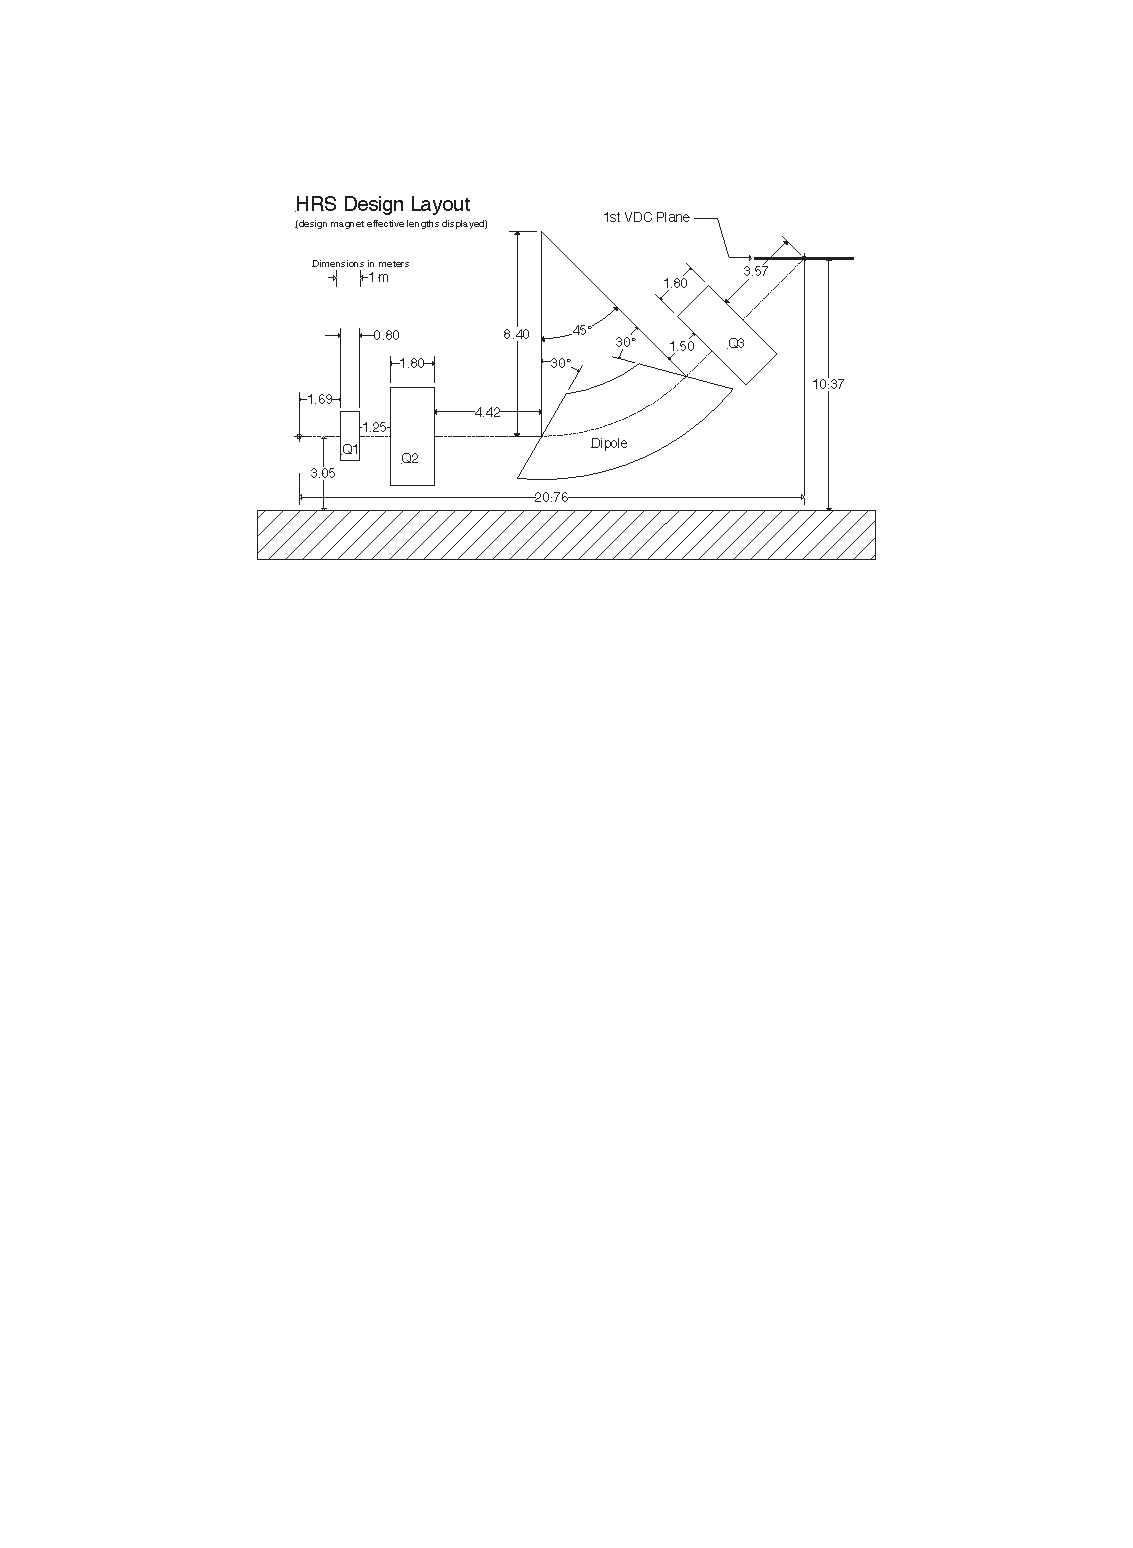
\includegraphics[width=0.9\textwidth]{figs/HRS.pdf}
\caption[HRS magnets layout]{The Hall A high resolution spectrometers magnets layout(sideview).  \label{fig:QQDQ_config}}
\end{figure}

\subsection{Collimator}
Each HRS spectrometer has a collimator box carefully aligned and rigidly attached to the entrance flange of the 
first quadruple.
In each collimator box, there are a set of collimators and a sieve slit.

The first two collimators are made of 80 mm thick tungsten, positioned around 1109 mm away from the target.
The first collimator has an aperture of 121.8(vertical) $\times$ 62.9(horizontal) mm at the entrance and
129.7(V) $\times$ 66.8(H) mm at the exit.
The second collimator is smaller and with an aperture of 50.0(V) $\times$ 21.3(H) mm at the entrance and 53.2(V) $\times$
22.6(H) mm at the exit.

The third collimator is called "sieve slit", which is used to determine the angular information during optics calibration.
It is made of 5 mm thick stainless steel sheet, positioned 1165.3 mm (LHRS) (or 1192.5 mm (RHRS)) away from Hall A center.
There are 49 holes (arranged in a 7$\times$7 array) on the sieve slit, spaced 25 mm apart vertically and 12.5 mm part horizontally.
Two of them big holes, one in the center and one displaced two rows vertically and one horizontally, are 4 mm in
diameter. The other holes are 2 mm in diameter.

\subsection{Detector Packages}
Following the third quadruple is the detector package.
The detector package is designed for various functions in the characterization of charged particles coming through the spectrometer.
For CSR experiment the detector package includes:

\begin{itemize}
\item A pair of Vertical Drift Chambers (VDCs) to determine the tracking information (momentum and trajectory);
\item Two scintillator planes, S1 and S2, to provide trigger to activate the data acquisition(DAQ) electronics;
\item A gas Cerenkov detector to provide particle identification (PID) information;
\item On LHRS, there is a NaI calorimeter to extract information on low energy electrons. 
Unfortunately, some blocks are unresponsive during the experiment due to the unsuccessful installation.
So the NaI was not used for data analysis.
\item A set of lead glass calorimeter for additional PID.
\end{itemize}

The layout of the LHRS and RHRS detector packages are shown in Figure.~\ref{fig:LHRS_detectors} and
Figure.~\ref{fig:RHRS_detectors}. The details of the detectors used in CSR experiment are explained below.

\begin{figure}[tb!]
\centering
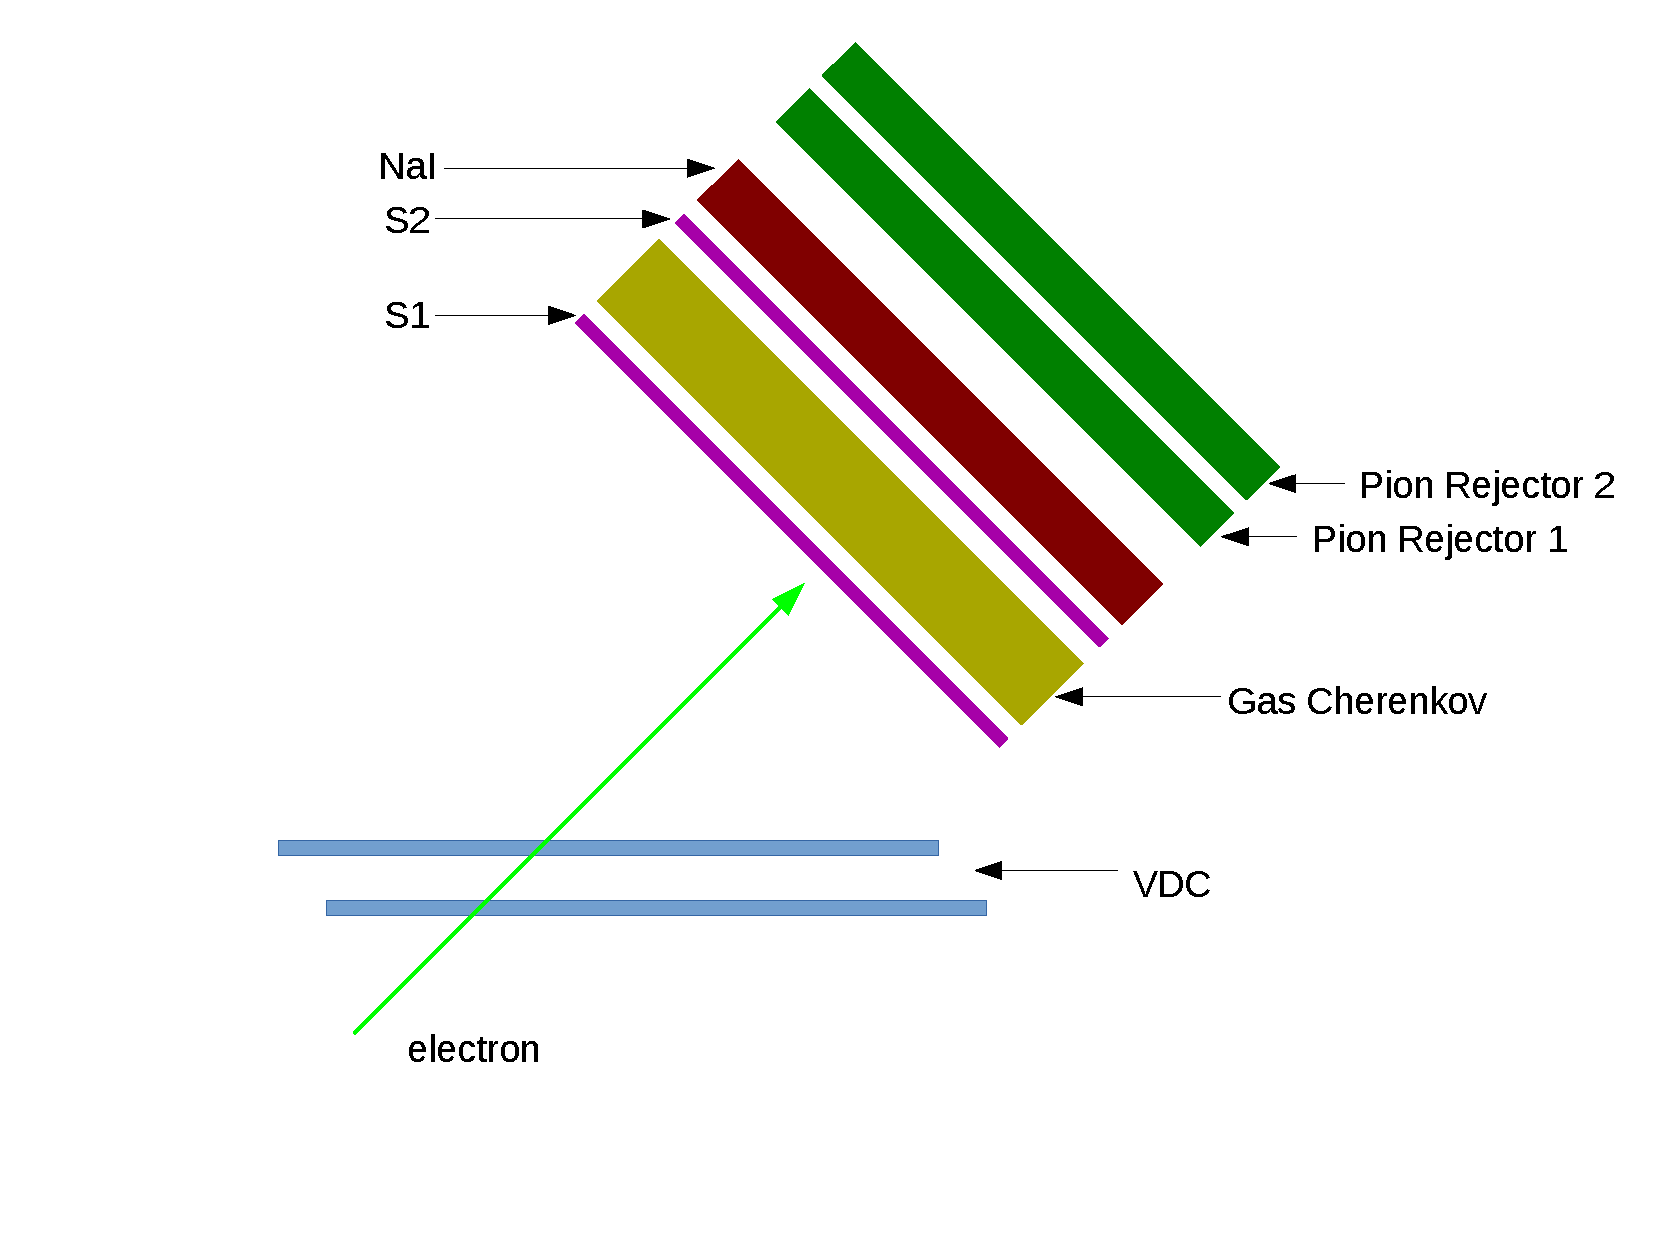
\includegraphics[width=0.5\textwidth]{figs/LHRS_detectors.pdf}
\caption[The LHRS detector package.]{The LHRS detector package.  \label{fig:LHRS_detectors}}
\end{figure}

\begin{figure}[tb!]
\centering
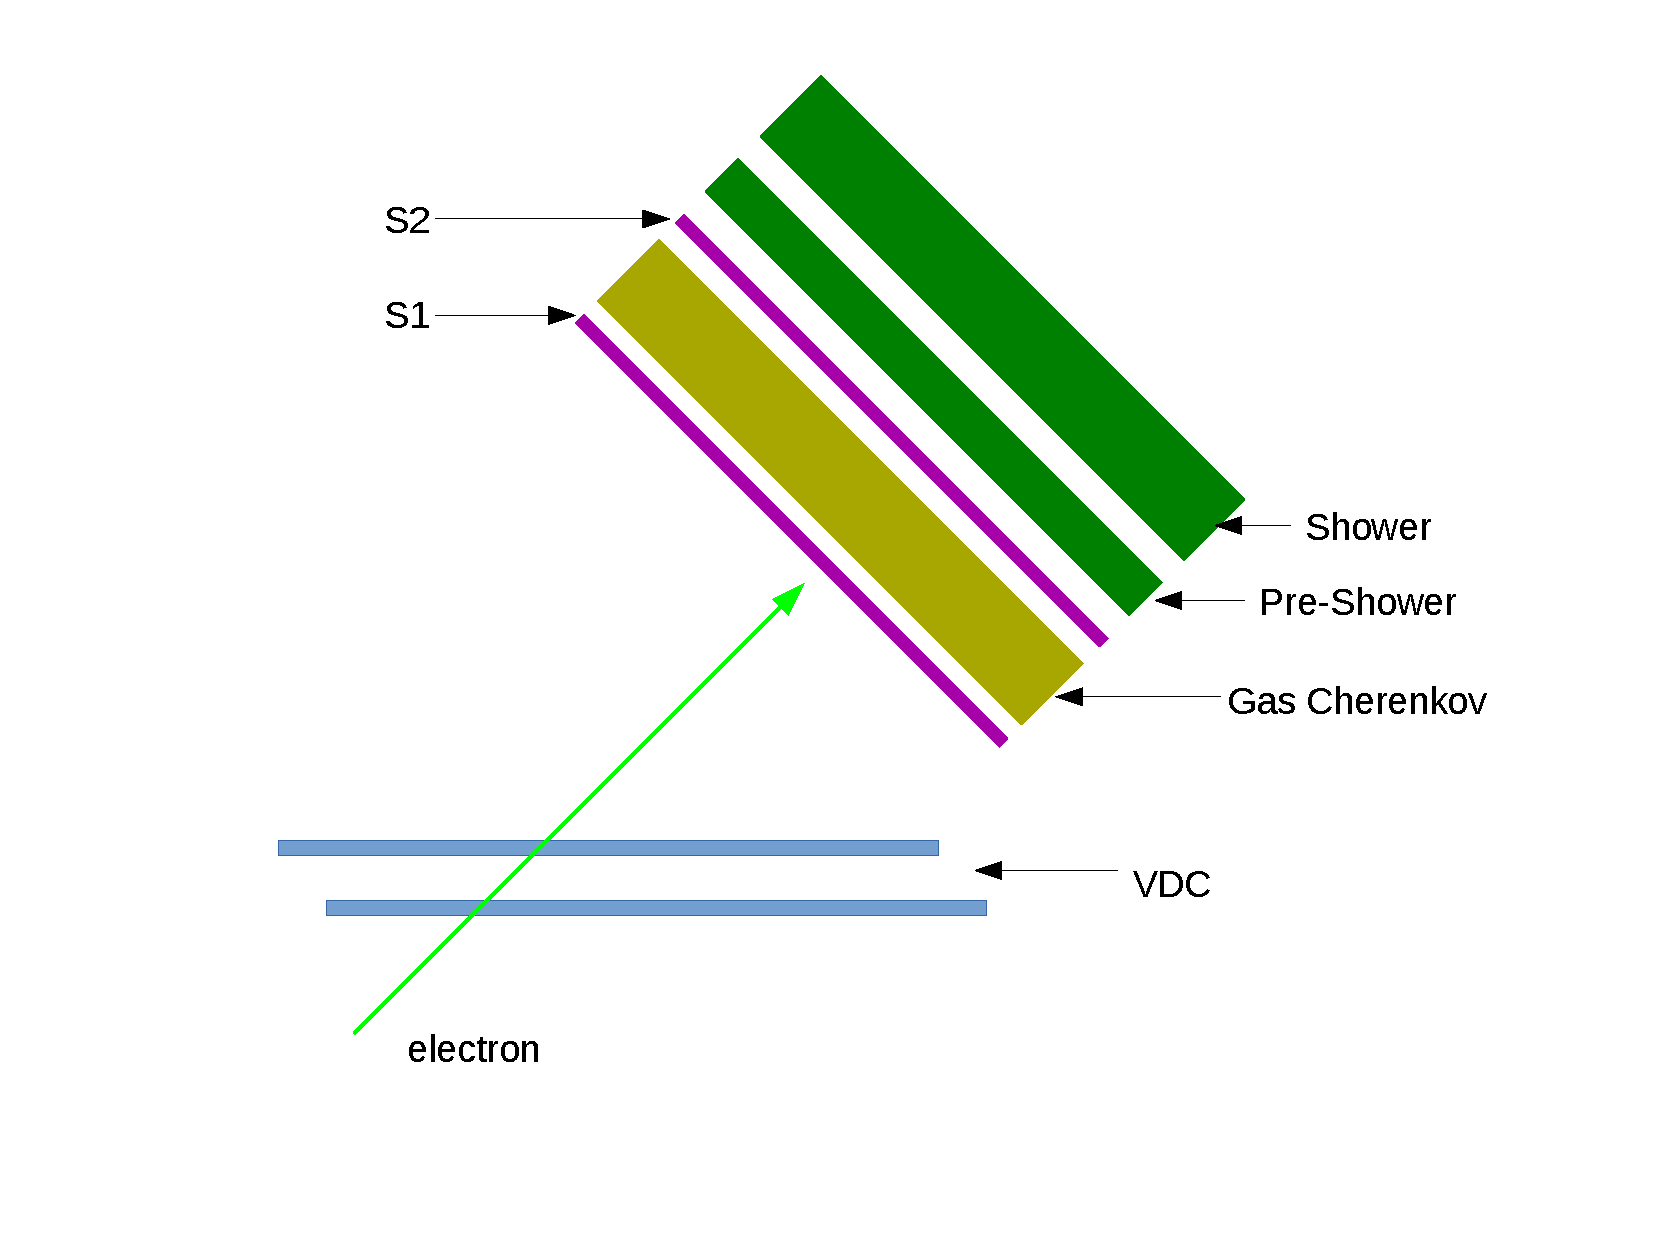
\includegraphics[width=0.5\textwidth]{figs/RHRS_detectors.pdf}
\caption[The RHRS detector package.]{The RHRS detector package.  \label{fig:RHRS_detectors}}
\end{figure}


\subsubsection{Vertical Drift Chamber}
%position and geometry
Each HRS spectrometer use a pair of Vertical Drift Chambers (VDC) to provide particle tracking information.
The layout of VDC is shown in Figure.~\ref{fig:VDC_layout}.

\begin{figure}[tb!]
\centering
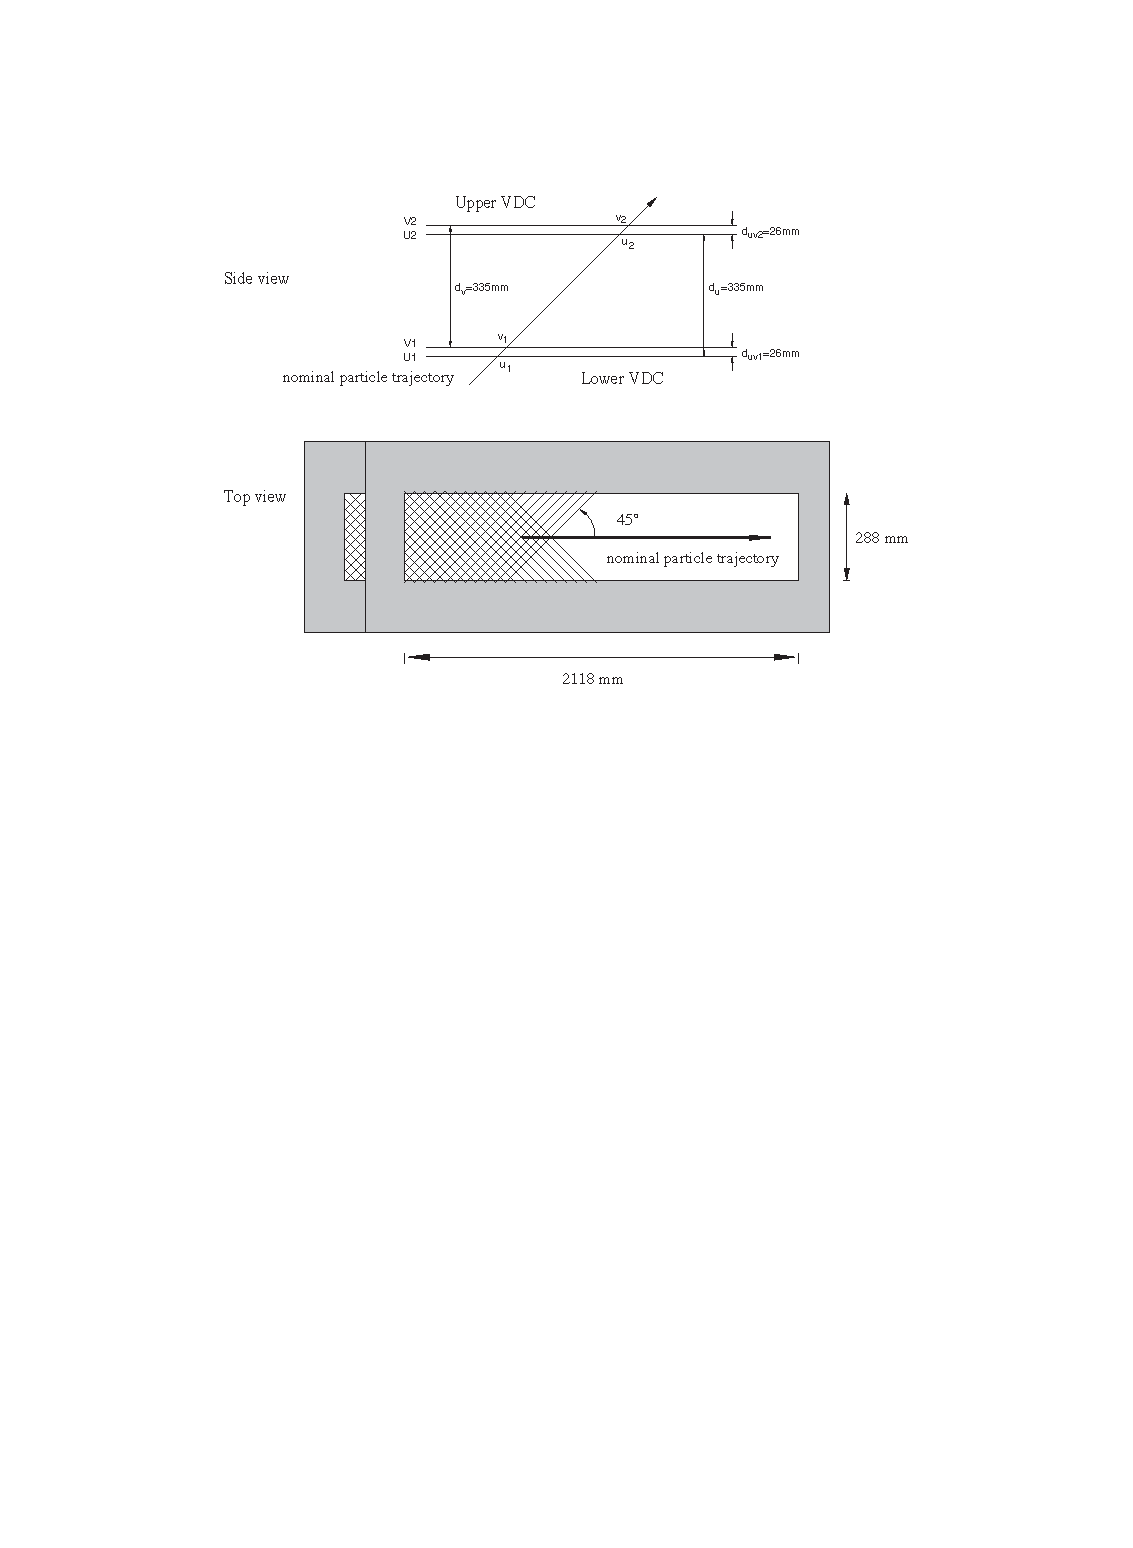
\includegraphics[width=0.8\textwidth]{figs/VDC.pdf}
\caption[Schematic layout of Vertical Drift Chambers]{Schematic layout of a pair of Vertical Drift Chambers.
\label{fig:VDC_layout}}
\end{figure}

The two VDC chambers are positioned 335 mm away from each other, each VDC has a standard U-V plane configuration.
The wires of one plane are \SI{90}{\degree} to that of the other plane, and lie in the laboratory horizontal plane.
They are inclined at an angle of \SI{45}{\degree} with respect to the dispersive(vertical) and non-dispersive(horizontal) directions.
The particle's central trajectory crosses the wire planes at an angle of \SI{45}{\degree}.
The distance between U and V planes is 26 mm, there are 368 sense wires in each plane, the spacing between two
adjacent wire is 4.243 mm.

%volt, gas, and signal
There are three high voltage gold-plated Mylar planes at about -4 kV in each VDC, one between U and V wire planes and two on opposite
sides, the wires are kept at ground voltage. The electric field between wires and cathode plane is show in Figure~\ref{fig:wire_chamber}.
The gas supply to the VDCs is a 62\% argon and 38\% ethane mixture. The gas is bubbled through cooled alcohol to reduce
aging effects on the sense wires \cite{Alcorn2004}. 

\begin{figure}[tb!]
\centering
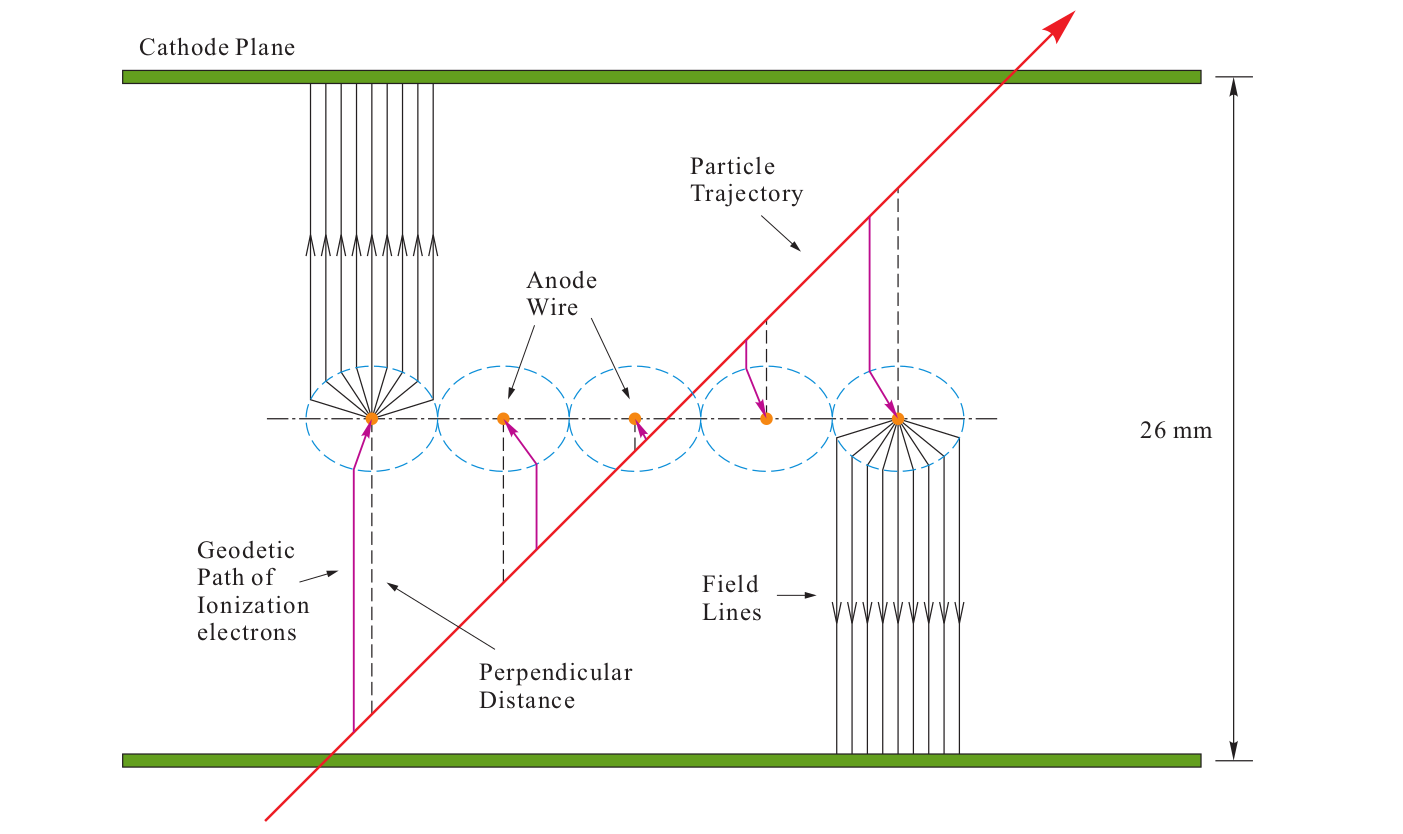
\includegraphics[width=0.8\textwidth]{figs/wire_chamber.png}
\caption[wire chamber]{Electric field between wires and cathode plane in VDC.
\label{fig:wire_chamber}}
\end{figure}

When an electron passes through the VDC planes, it ionizes the gas inside the chamber and leave behind ions and
generated electrons on it track. The generated electrons are drifted towards the sense wires with a constant velocity
(50 $\mu$m/ns) along the path of the least time, and accelerate rapidly near the wire producing a shower of secondary ionization.
This generates an electric signal on the sense wires. The timing information of the signal is measured by the Time-To-Digital
Converter (TDC), which is started by a triggered wire and stopped by the event trigger supervisor.
Since the ionization electron drift velocity is constant, the drift distance from trajectory to the wire can be
extracted from the TDC output. The trajectory can be reconstructed by combining drift distances of all fired wires.
By design, the charged particle crosses the VDCs at the nominal angle of \SI{45}{\degree} typically triggers 5 wires.
Considering the inefficiency of sense wires, the signals from 3 hits are also accepted as good track. 
The position and angular reconstruct resolution of focal plane are approximately 100 $\mu$m and 0.5 mrad, respectively.

\subsubsection{Scintillators and Trigger}
Two scintillator planes, S1 and S2, separated by 2 m, are used to generate the trigger for the DAQ system.
The active volume dimension of S1 and S2 are 36.0 cm (transverse or horizontal direction) $\times$ 29.3 cm (dispersive
or vertical direction) $\times$ 0.5 cm (thickness), and 60.0 cm (horizontal) $\times$ 37.0 cm (vertical) $\times$ 0.5
cm (thickness), respectively.
Each scintillator consists of 6 overlapping scintillator paddles made of thin plastic scintillators. 
Two photomultipliers (PMT) are attached to each scintillator paddle, one on left side and another on right side.
The time resolution of each plane is around 0.3 ns.

Charged particles coming through a scintillator paddle may generate scintillating light which travels towards
PMTs on both sides. Signals from PMTs are used to generate triggers and sent to all other detectors and the DAQ system.
To select good events for the analysis, each event is assigned an event type, with values from 1 to 5, based on the 
the scintillator signals as follows: 

\begin{itemize}
\item A T1(T3) event for the right(left) arm is considered to be a "good event". It satisfies the following conditions:
  \begin{enumerate}
    \item A scintillator paddle is called "fired" if PMTs on its both sides have signals;
    \item The N$_1$$^{th}$ paddle of S1 and N$_2$$^{th}$ paddle of S2 are "fired" within a specific time window;
    \item N$_2$$^{th}$ = N$_1$$^{th}$ or N$_2$$^{th}$ = N$_1$$^{th}$ $\pm$ 1. This means the angle formed by the particle trajectory
    and the central ray of the spectrometer is very small, or the trajectory is at approximately \SI{45}{\degree} with respect to the Hall floor.
  \end{enumerate}

 \item A T2(T4) event for the right(left) arm is formed if \textit{one of} the follwing conditions is satisfied:
  \begin{enumerate}
  \item The N$_1$$^{th}$ of S1 and N$_2$$^{th}$ of S2 are fired at the same time, but
        N$_2$$^{th}$ $\neq$ N$_1$$^{th}$ and N$_2$$^{th}$ $\neq$ N$_1$$^{th}$ $\pm$ 1;
  \item Either S1 or S2 is fired, at the same time Gas Cerenkov fires.
  \end{enumerate}
  T2(T4) events are either cosmic ray events, or particles on the edge of the acceptance.

 \item A T5 event is defined as the coincidence event of T1 and T3. It was not used during the CSR experiment.
\end{itemize}

Triggers T1-T4 are counted by scalers and are sent to the trigger supervisor. The trigger supervisor sychronizes all the
detector read-out and send them to the DAQ system. Because of the hardware limitation of DAQ system, it cannot record all
events when event rate is high. A quantity called livetime(LT) is defined as the fraction of events
recorded by DAQ, given by:

\begin{equation} \label{LT_def}
LT = \frac{\mathrm{number \; of \; events \; that \; are \; recorded \; by \; DAQ}}{\mathrm{number \; of \; events \; that \; are \; fed
\; to \; DAQ}}
\end{equation}
If the event rate is very high, events can be prescaled by an integer prescale factor $p_{1(2,3,4)}$ for $T_{1,2,3,4}$ at the trigger supervisor to decrease the
load of DAQ system. Only one event is sent to the DAQ system for each set of $p_{1(2,3,4)}$ subsequent events.
Livetime is event type dependent. It can be found by comparing the number of triggers $T_{1(2,3,4)}$ recorded by scalers
and the total number of triggers accepted by the DAQ system, $T_{DAQ,1(2,3,4)}$:

\begin{equation}
LT_{1,(2,3,4)} = \frac{p_{1,(2,3,4)}T_{DAQ,1(2,3,4)}}{T_{1(2,3,4)}}
\end{equation}  

Similarly, we can define a quantity called trigger inefficiency which describes the fraction of 
"good events" miscounted as T2(T4) events.
To minimize the dilutions from cosmic events, we usually choose a high yield run.
The trigger inefficiency is defined as:

\begin{equation}
\mathrm{Inefficiency} = \frac{T_{2(4)}}{T_{1(3)} + T_{2(4)}}
\end{equation}  

Then the trigger efficiency can be extracted as:

\begin{equation}
\eta_{trig} = 1 - \mathrm{Inefficiency} =  \frac{T_{1(3)}}{T_{1(3)} + T_{2(4)}}
\end{equation}  

The trigger inefficiencies for both left and right arms are below 1\% during CSR experiment
and are negligible.


\subsubsection{Gas Cerenkov Detector}
Gas Cerenkov detector is used for particle identification in CSR experiment.
The Gas Cerenkov detector is based on Cerenkov effect.
When a charged particle passing through a dielectric medium with a refraction index n, it polarizes atoms
along its tracks so that they become dipoles. Those atoms return to unpolarized state by emitting photons
after the electron passage. If $v < c/n$, the dipoles are symmetric with respect to the particle's path,
the destructive interference happens and there will be no radiation. However, if $v > c/n$, the symmetry is broken
and constructive interference happens, which will cause a radiation at the fixed angle $\theta_c$ with respect to the particle's trajectory.  
Figure~\ref{fig:Cerenkov-radiation} shows the geometry of the emission of Cerenkov radiation.

\begin{figure}[!htp]
\centering
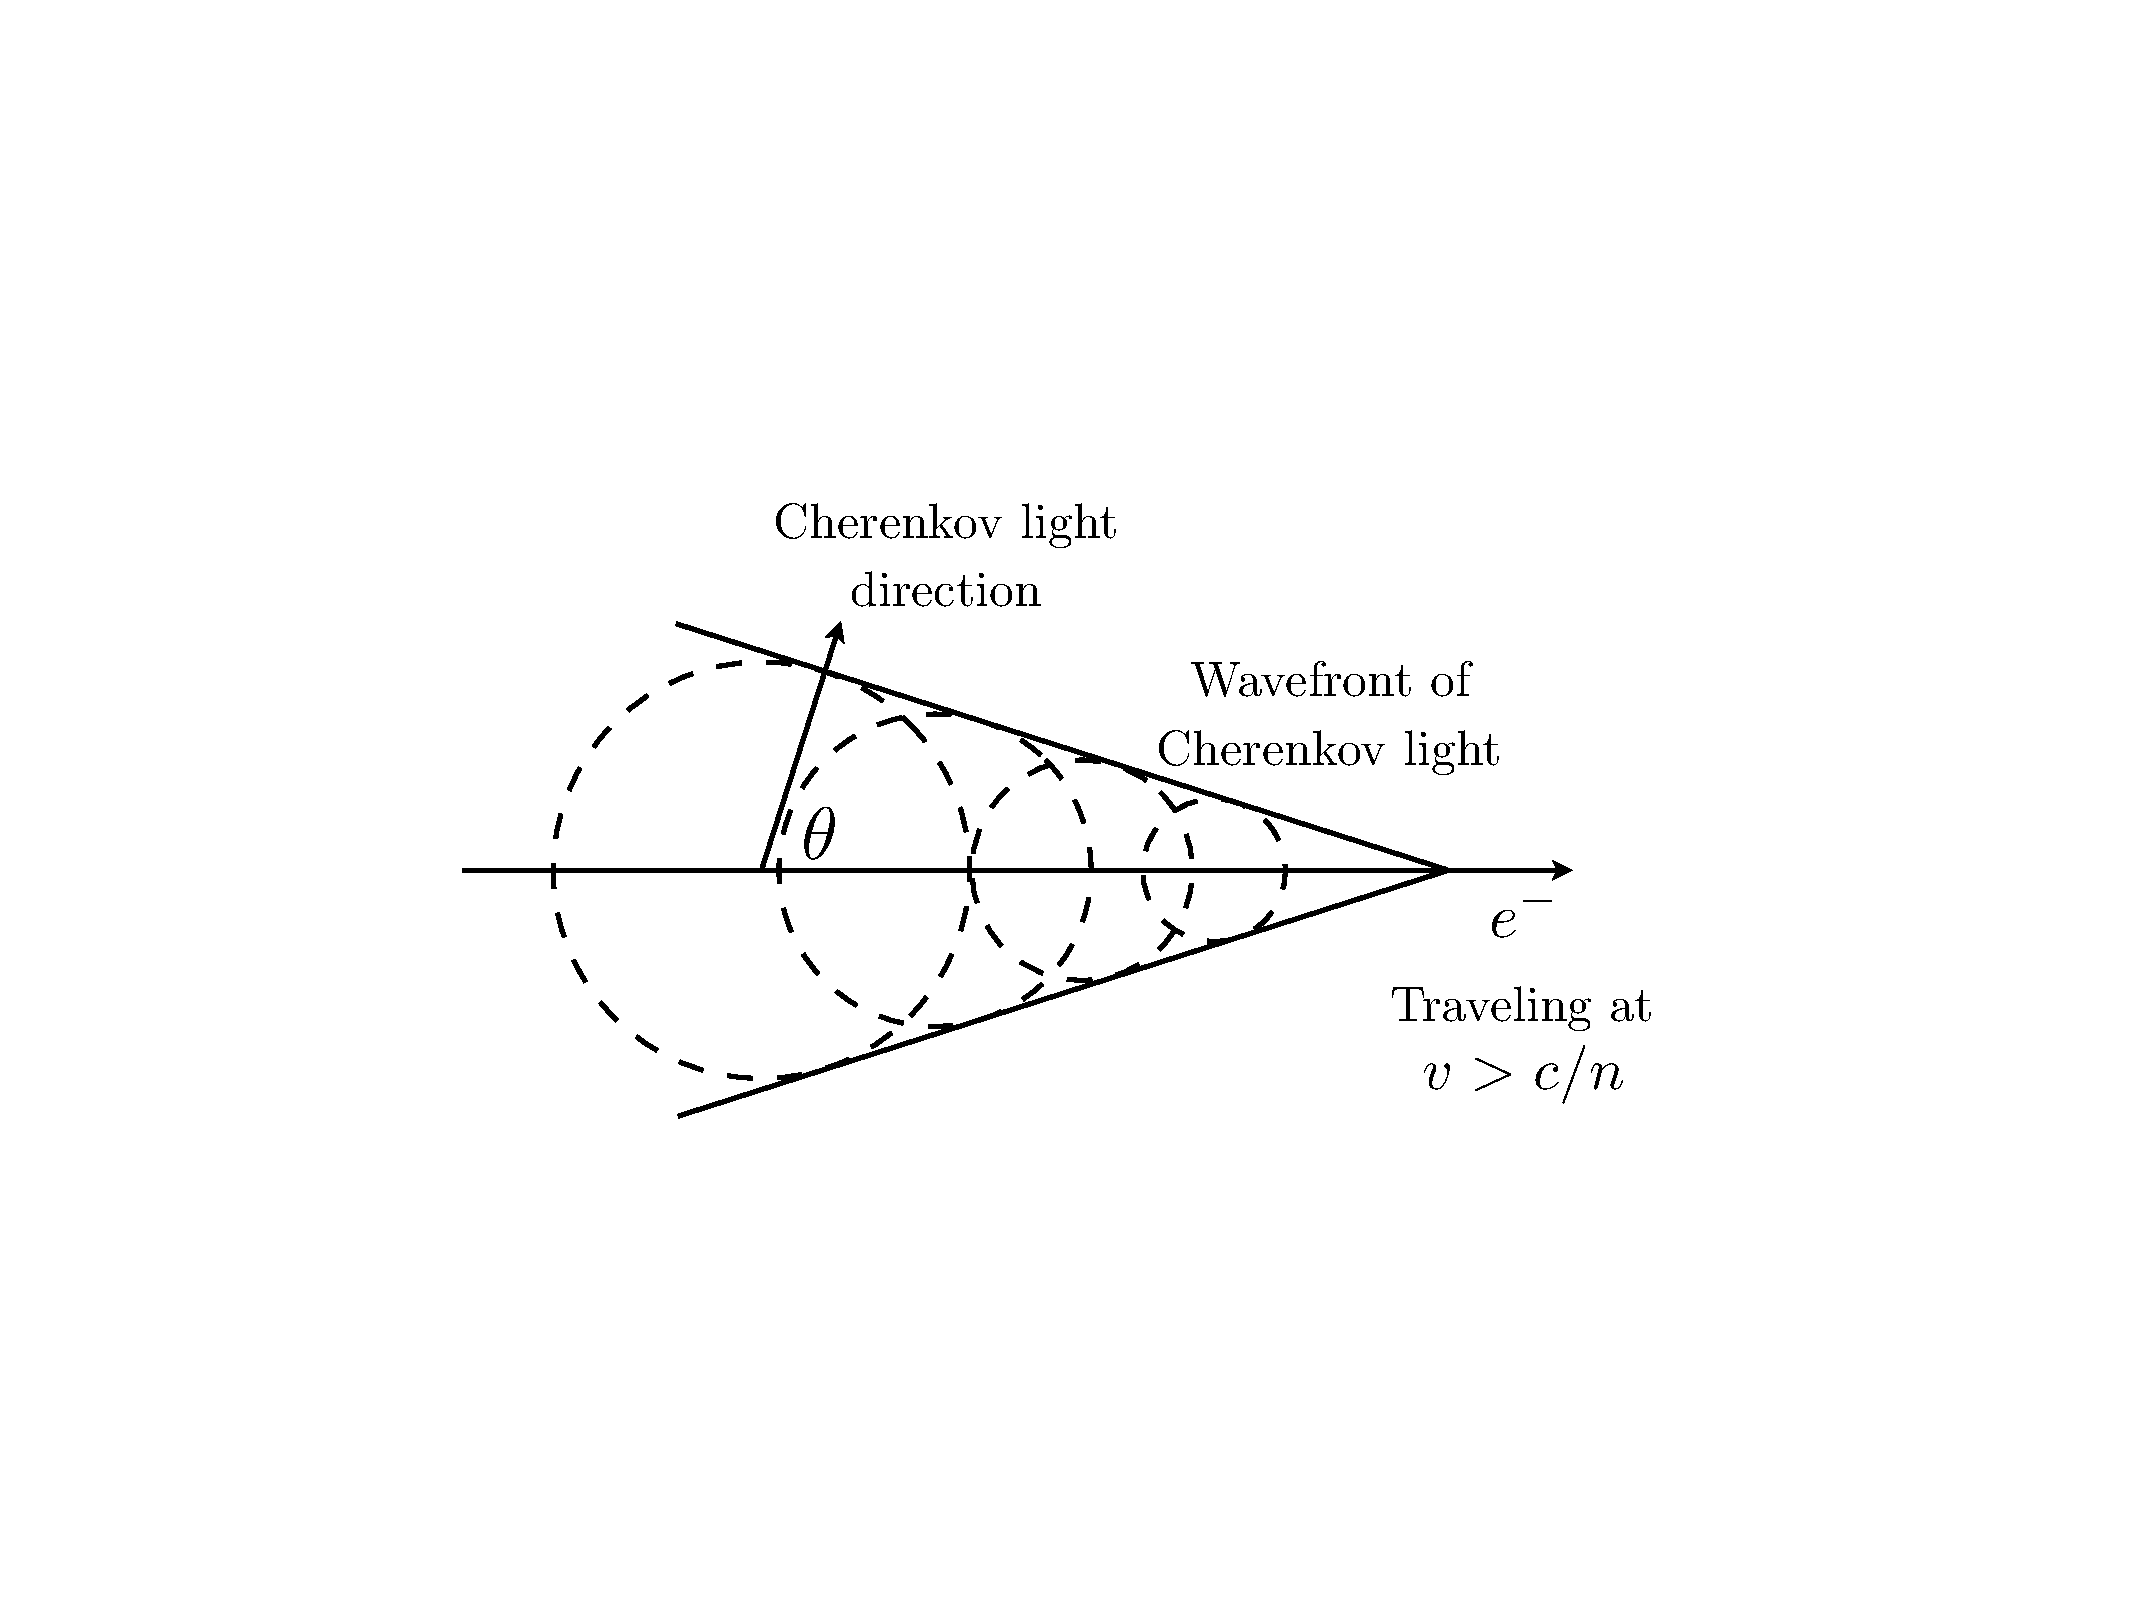
\includegraphics[width=0.6\textwidth]{figs/Cherenkov-radiation.pdf}
\caption[Cerenkov radiation]{The geometry of the emission of Cerenkov radiation.
\label{fig:Cerenkov-radiation}} 
\end{figure}

The threshold velocity and momentum for the production of Cerenkov light are given by:

\begin{equation} \label{Cerenkov_theshold_v}
\beta_{min} c = \frac{c}{n}
\end{equation}

\begin{equation} \label{Cerenkov_theshold_p}
p_{min} = \frac{mc}{\sqrt{n^2-1}}
\end{equation}

The threshold angle $\theta_c$ is given by: 

\begin{equation} \label{Cerenkov_direction}
\cos \theta_c = \frac{1}{\beta_{min} n}
\end{equation}

By detecting if a particle emit Cerenkov light, one can know if this particle's velocity is larger than threshold velocity
in the medium.


%with refraction index n, if the
%speed of particle $v = \beta c$ is higher than the speed of light $\frac{c}{n}$ in this medium,
%the particle will emit electromagnetic radiation called the Cerenkov light.
%Cerenkov light is emitted because the material becomes electrically polarized by the particle's electric field.
%If the speed of particle exceed the speed of light in the material, the 

During the CSR experiment the main background is pion. The Cerenkov detector can be used to separate 
electrons from pion background.
The gas Cerenkov detector is filled with CO$_2$ at atmospheric pressure.
With a refraction index n = 1.00041, the threshold momentum of electron and pion are:
\begin{equation} 
p_e = 17 \mathrm{MeV}/c, \;\; \mathrm{and} \;\;\;  p_{\pi} = 4.8 \mathrm{GeV}/c.
\end{equation}
Because the beam energy of CSR experiment range from 0.4 to to 4 GeV only electrons generate signals in the
Cerenkov and pions do not. The gas Cerenkov detector has an efficiency higher than 99\% in
identifying electrons.

The gas Cerenkov detector for each arm is installed between two scintillator planes, S1 and S2.
It is made of steel with thin entrance and exit window made of tedlar.
There are ten spherical mirrors installed as 5 (vertical) $\times$ 2(horizontal) arrray,
to focus the Cerenkov light on ten PMTs.
The mirrors have radius of curvature of 90 cm, and the PMTs are placed at $f=$90/2 = 45 cm from the mirrors,
such that parallel incident light can be focused on PMTs.
Signals from PMTs are sent to ADCs and summed together.
Even though pions cannot produce Cerenkov light, but they still can ionize the gas medium 
and thus generate secondary electrons. These secondary electrons may have high enough energy to trigger
Cerenkov detector and leave a background signal that lies near the single-photon-electron peak.
This background can be removed in the analysis using ADC cuts which will be explained in Chapter 4(Data Analysis).


\subsubsection{Electromagnetic Calorimeters}
The electromagnetic calorimeters provide an additional way of PID. When a high energy charged particle travels through 
lead glass, it will create a shower of photons and e$^-$/e$^+$ pairs. The photons created in this cascade process
will be collected by PMTs and the signal intensity is linearly proportional to the energy deposit of the incoming particle.
There will be two peaks in the output spectra, one peak with higher energy for electrons and another peak with lower energy
for pions. The double-layer configuration can provide PID because the second layer of lead glass calorimeter can further
separate electrons from contamination of pions.

The configurations of lead glass calorimeters on the LHRS and RHS are slightly different, see
Figure.~\ref{fig:calorimeters}.
The lead glass calorimeters on LHRS is composed of two layer of lead glass blocks with same geometry, each layer is called
a "pion rejector". Each layer consists of 17 long blocks and 17 short blocks, forming a 17(dispersive) $\times$
2(transverse) array, with dimension 14.5 cm $\times$ 14.5 cm $\times$ 30(or 35) cm.
Short blocks(30 cm long) and long blocks(35 cm long) are arranged interchangeablely in the dispersive direction for each row.

\begin{figure}[tb!]
\centering
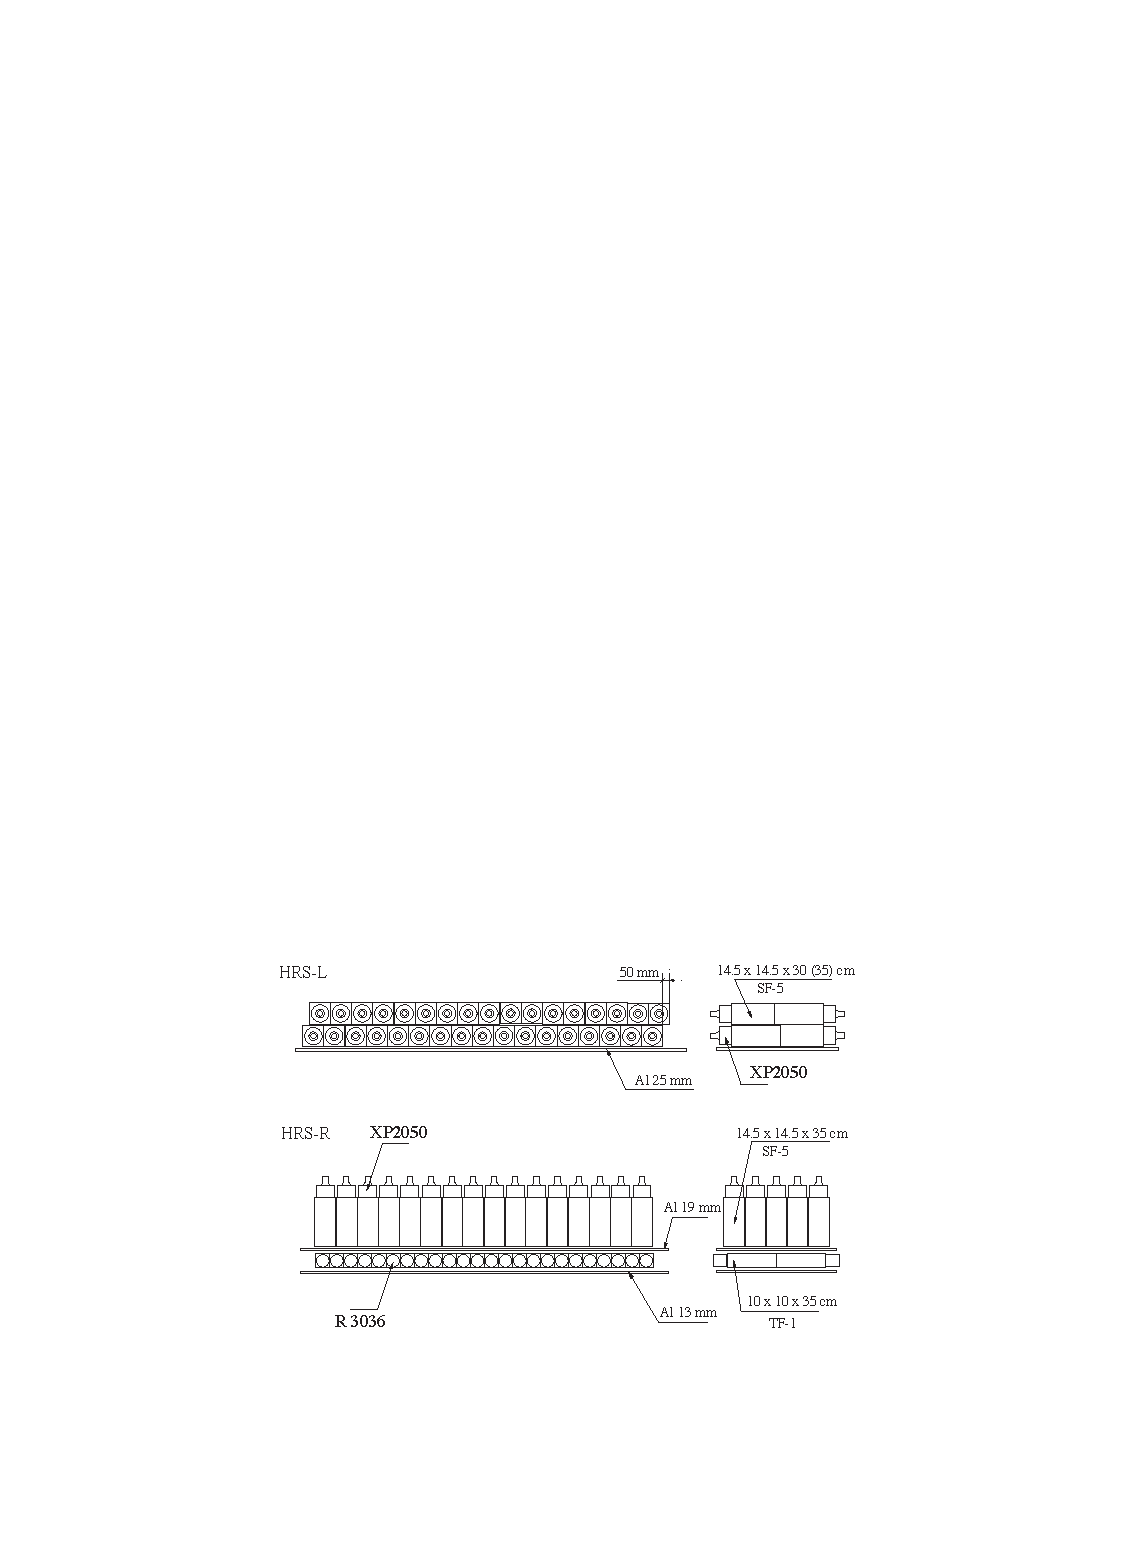
\includegraphics[width=0.8\textwidth]{figs/calorimeters.pdf}
\caption[Layout of electromagnetic calorimeters]{Schematic layout of electromagnetic calorimeters in left and right HRS.  \label{fig:calorimeters}}
\end{figure}

On the RHRS, the two layers are called "preshower" and "shower" respectively.
The first layer of lead glass blocks, "preshower", is arranged in an array of 24(dispersive) $\times$ 2 (transverse),
with dimension 35 cm $\times$ 10 cm $\times$ 10 cm, with the lead glass blocks perpendicular to the direction of
incoming electrons.
The "shower" is composed of 16(dispersive) $\times$ 5(transverse) blocks, with dimension 35 cm $\times$ 15 cm $\times$ 15 cm
which are oriented parallel to the electron trajectory.

The main difference between LHRS and RHRS lead-glass calorimeters is that the RHRS calorimeter is thick enough that 
electrons will deposit all their energies, while the calorimeter on LHRS is not a full energy absorber because of its
reduced thickness.


\section{Data Acquisition System}
The Data Acquisition system is used to collect event information from the detectors and beamline apparatus
and store the raw data.
The Hall A DAQ system is built on CEBAF Online Data Acquisition System (CODA), a software package specifically for
developed nuclear physics applications by the JLab data-acquisition group.  

CODA is composed of a set of software packages which can control DAQ hardwares such as front-end Fastbus VME digitization
devices (ADCs, TDCs, scalers), the VME Interface to Fastbus, single-board VME computers, and mass storage system(MSS).
%The custom software components of CODA are shown in Figure:
%A readout controller (ROC) runs on the front-end crates 
The raw data are divided into different runs for specific kinematics settings. Each run consists of several parts of
information:
\begin{itemize}
\item A header consists of information like run number, timestamp, event size and prescale factors.
\item CODA events which contain detectors and helicity information.
\item EPICS events contains information about beamline apparatus, spectrometer magnets setting and angle, target information
and other slow control device.
\item Scaler events which contain number of triggers and accumulated charges of the run.
\end{itemize}

\begin{figure}[tb!]
\centering
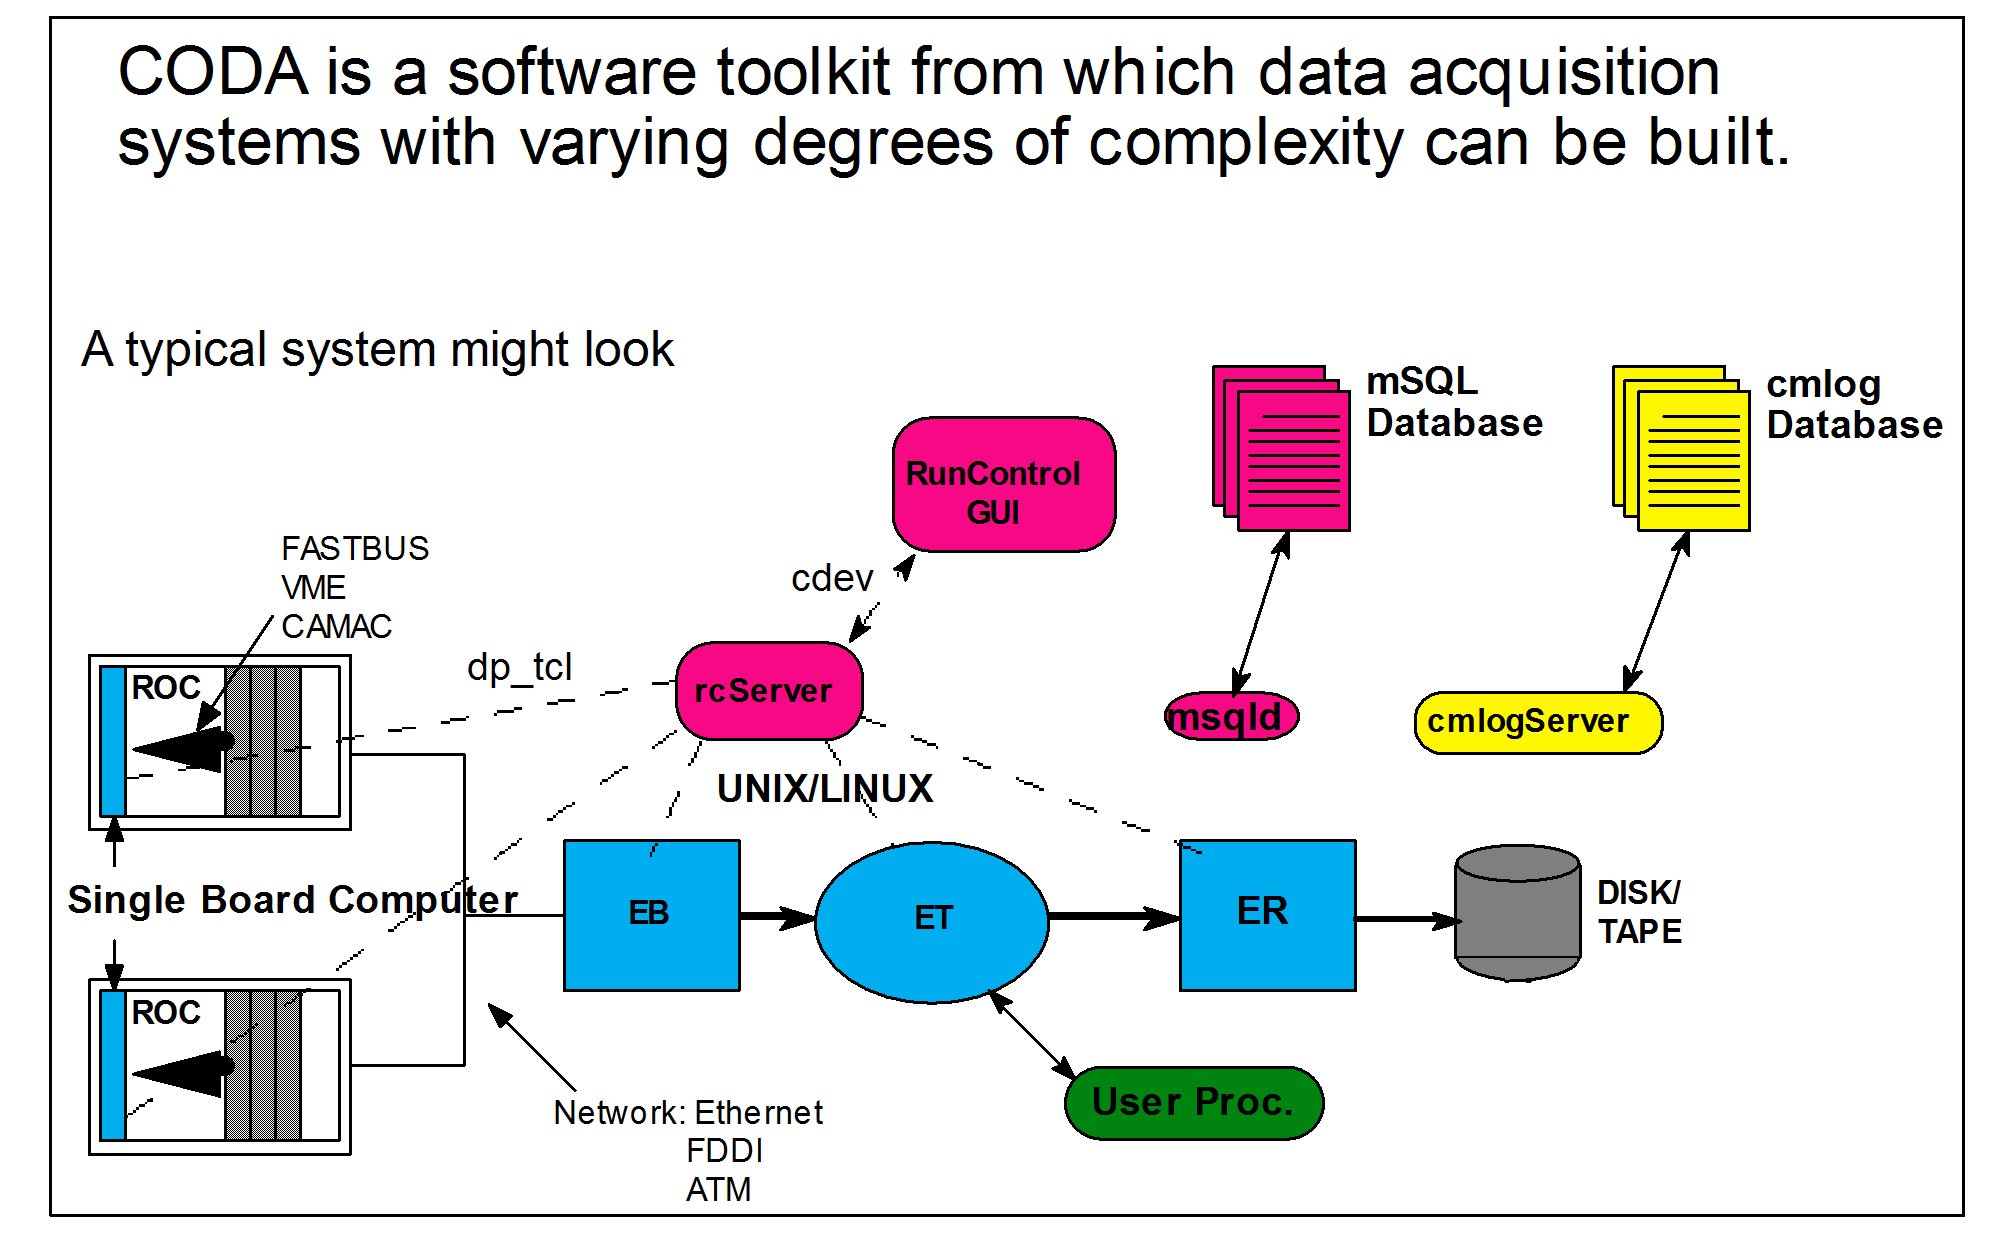
\includegraphics[width=0.8\textwidth]{figs/DAQ_diagram.png}
\caption[DAQ system diagram]{DAQ system diagram.  \label{fig:daq_diagram}}
\end{figure}

The data is first written to a local disk then moved to the Jefferson Lab Mass Storage System (MSS).
The total volume of data accumulated during the CSR experiment was about 3.0 TBytes.
%
%
%
%
%\cite{*}
%
%%%%%%%%%%%%%%%%%%%%%%%%%%%%%%%%%%%%%%%%%%%%%%%%%%%%%%%%%%%%%%%%%%%%%%%
%% -*-latex-*-

%% -*-latex-*-

%% This is an example first chapter.  You should put chapter/appendix that you
%% write into a separate file, and add a line \include{yourfilename} to
%% main.tex, where `yourfilename.tex' is the name of the chapter/appendix file.
%% You can process specific files by typing their names in at the
%% \files=
%% prompt when you run the file main.tex through LaTeX.

\chapter{Data Analysis}
\label{Data_Analysis}

In this chapter, we will discuss the data analysis procedures
of Coulomb Sum Rule Experiment (E05110).

%%%%%%%%%%%%%%%%%%%%%%%%%%%%%%%%%%%%%%%%%%%%%%%%%%%%%%%%%%%%%%%%%%%%%%
\section{Optics Calibration}
\label{Optics_Calibration}

The Hall A HRS are two spectrometers each with an identical group of superconducting magnets,
three quadrupoles and a dipole in a QQDQ configuration as mentioned in the previous chapter.
The optics matrix is used to reconstruct the interaction vertex at the target from coordinates
of detected particles at the focal plane. This section will discuss the optics calibration procedure
used to determine the optics matrix elements.

\subsection[Coordinate System]{Coordinate System}
\label{Coordinate_System}
In this section, some coordinate systems used in optics calibration are
introduced. More details of these coordinate systems can be found in .
%~\cite{NIM}.

Note that an reference to an angular coordinate should be taken to refer
to the tangent of the angle.

\subsubsection{Hall Coordinate System(HCS)}

The origin of HCS is at the center of Hall A, which is the intersection of
beamline and vertical symmetric axis of the target system. The z axis is
along the beamline and pointing to the beam dump, the x axis is pointing to
the left of the beam, and the y axis is pointing up (See Figure.~\ref{fig:hcs}).

\begin{figure}
  \begin{center}
	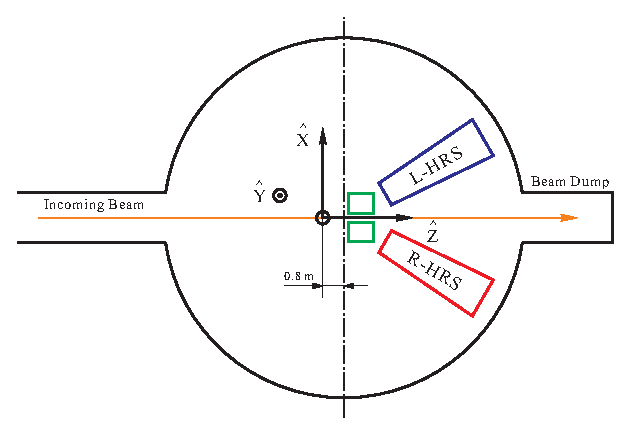
\includegraphics[scale=0.8]{figs/hcs}
  \end{center}
  \caption[Top view of hall coordinate sytem]
  {Top view of hall coordinate system.}
  \label{fig:hcs}
\end{figure}

\subsubsection{Target Coordinate System(TCS)}

Each of the spectrometers has its own TCS coordinate. The z axis of TCS is
along spectrometer center line and perpendicular to the sieve slit surface,
pointing from target. The y axis is going through the origin, pointing to 
the left side of z axis. x axis is pointing down vertically.(See
Figure.~\ref{fig:tcs}) In ideal case,
the origin of TCS is pointing to the Hall center, the origin of TCS and HCS
are same. In the experiment, the HRS central ray is not ideally pointing to
the Hall center, there is a horizontal shift $D_y$ and vertical shift $D_x$.
These shifts are measured in survey. The distance from TCS origin to the
center of collimator is defined as a constant, L. The in-plane angle of a
trajectory $\theta_{tg}$ is defined as $\frac{x_{sieve}}{L}$, and the out-of
-plane angle $\phi_{tg}$ is defined as $\frac{y_{sieve}}{L}$.

\begin{figure}
  \begin{center}
	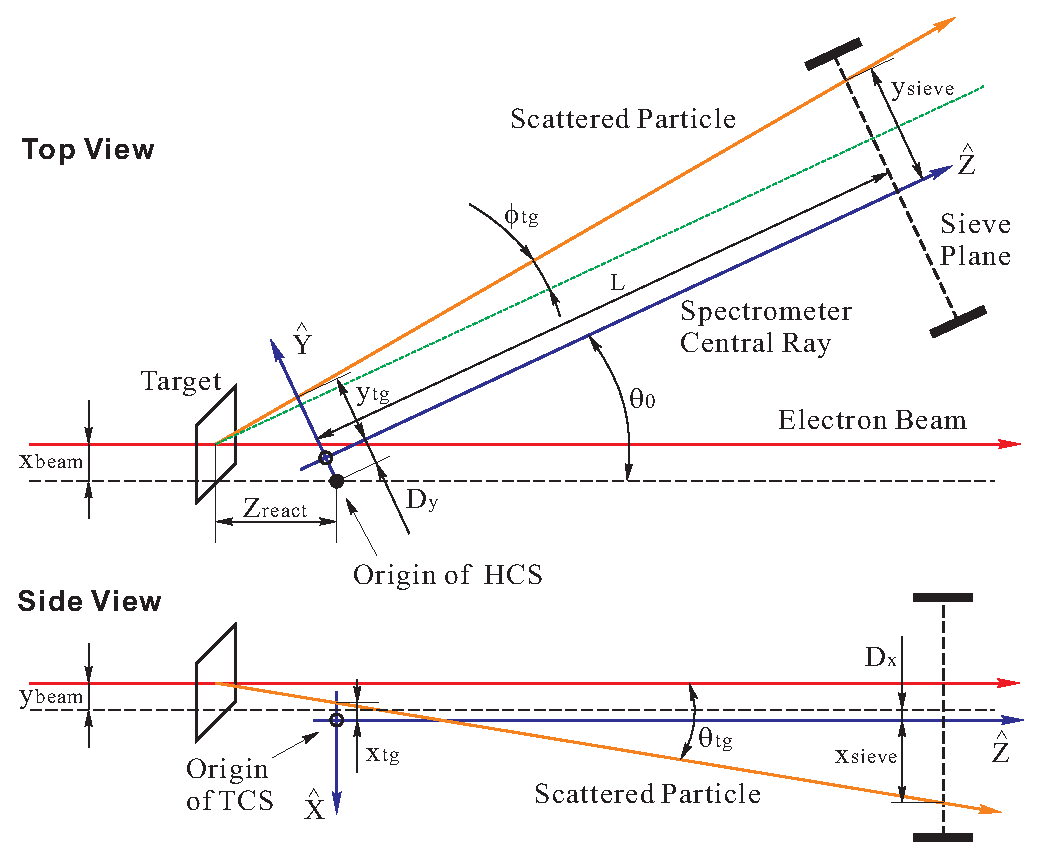
\includegraphics[scale=0.8]{figs/tcs}
  \end{center}
  \caption[Top and side view of target coordinate sytem]%
  {Top and side view of target coordinate sytem.}
  \label{fig:tcs}
\end{figure}

\subsubsection{Detector Coordinate System(DCS)}

The origin of DCS is defined by the wire 184 of VDC U1 plane and wire
184 of VDC V1 plane's projection on U1 plane. The $z$ axis is perpendicular
to the VDC plane, the $x$ axis is along the long symmetry axis and pointing
to the dispersive direction (See Figure.~\ref{fig:dcs}).
The coordinate of the detector vertex can be calculated from the
intersection points on four VDC planes(U1, V1, U2, V2):
  \begin{align}
  \tan (\eta_1) = \frac{p_{U2} - p_{U1}}{d2} \\
  \tan (\eta_2) = \frac{p_{V2} - p_{V1}}{d2} \\
  \theta_{det} = \frac{1}{\sqrt{2}} (\tan(\eta_1)+\tan(\eta_2)) \\
  \phi_{det} = \frac{1}{\sqrt{2}} (-\tan(\eta_1)+\tan(\eta_2))  \\
  x_{det} = \frac{1}{\sqrt{2}}{p_{U1}+p_{V1}-d_1 \tan(\eta_2)}  \\
  y_{det} = \frac{1}{\sqrt{2}}{-p_{U1}+p_{V1}-d_1 \tan(\eta_2)} 
  \end{align}

\begin{figure}
  \begin{center}
	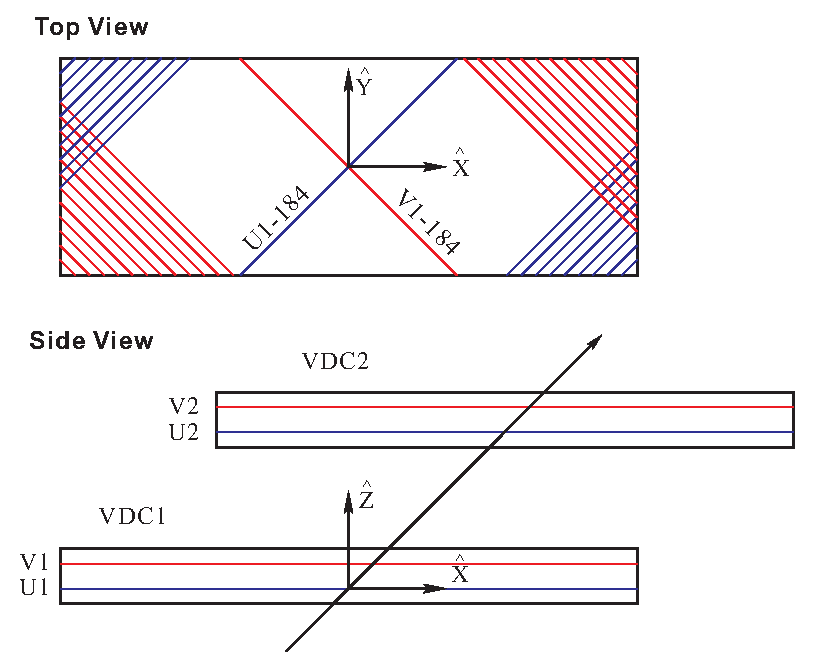
\includegraphics[scale=0.8]{figs/dcs}
  \end{center}
  \caption[Top and side view of detector coordinate sytem]%
  {Top and side view of detector coordinate sytem.}
  \label{fig:dcs}
\end{figure}

\subsubsection{Target Transport Coordinate System(TRCS)}

The TRCS is generated by rotating DCS clockwise along its $y$ axis by
45$^\circ$ (see Figure.\ref{fig:trcs}). So the $z$ axis of TRCS will
coincides with the central trajectory of the spectrometer in the ideal case.
It is a middle step from DCS to Focal Plane Coordinate(FCS) which will be 
described in next section. The transform from DCS variable to TRCS variables
can be expressed by:

\begin{figure}
  \begin{center}
	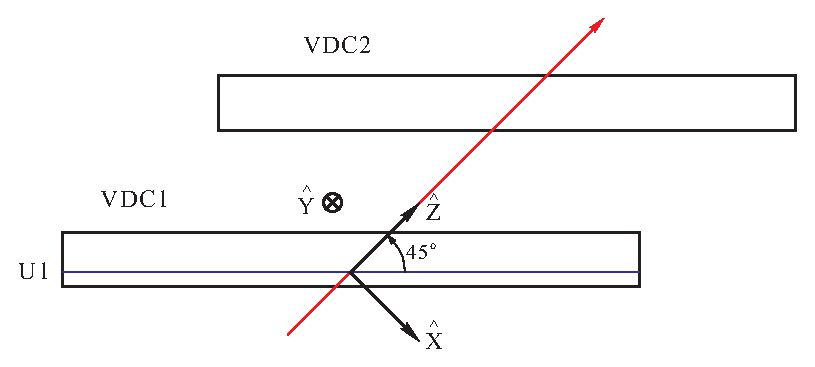
\includegraphics[scale=0.8]{figs/trcs}
  \end{center}
  \caption[Transport coordinate sytem]%
  {Transport coordinate system.}
  \label{fig:trcs}
\end{figure}

\begin{align}
x_{tra}     = x_{det}\cos(\rho_0)(1+\theta_{tra}\tan(\rho_0)) \\  
\theta_{tra}= \frac{\theta_{det}+\tan(\rho_0)}{1-\theta_{det}\tan(\rho_0)} \\  
y_{tra}     = y_{det}+\sin(\rho_0)\phi_{tra}x_{det} \\ 
\phi_{tra}  = \frac{\phi_{det}}{\cos(\rho_0)(1-\theta_{det}\tan(\rho_0))}
\end{align}

where $\rho_0$ = 45$^\circ$ is the rotation angle.

\subsubsection{Focal Plane Coordinate System(FCS)}

Because the focusing of the dipole in HRS magnet system, particles
from different scattering angle will be focused at focal plane. So the
relative momentum $\delta$ (defined in equation ~\ref{equ:dp}) mostly
depends on the location in dispersive direction, $x_{det}$. 

\begin{equation}
\delta = \frac{p-p_0}{p_0}
\label{equ:dp}
\end{equation}

FCS is a rotated coordinate system,
it is generated by rotating the DCS for a varying angle, $\rho(x_{tra})$,
so the new $\hat{z}$ axis is along to the local central ray, which has
$\theta_{tg}$=0 and $\phi_{tg}$=0 (see Figure.~\ref{fig:fcs}).
With this rotation, the $\theta_{fp}$ is small for all points on focal
plane and approximately centered around $\theta_{fp}$=0.
This will ensure the expansion of the optics matrix will converge faster
during the optimization procedure.

The FCS variables can be expressed as: 

\begin{align}
x_{fp} = x_{tra}
\tan(\rho) = \Sigma t_{i000} x_{fp}^i \\
y_{fp} = y_{tra} - \Sigma y_{i000} x_{fp}^i \\
\theta_{fp} = \frac{x_{det}+\tan(\rho)}{1-\theta_{det}\tan(\rho)} \\
\phi_{fp} = \frac{\phi_{det}-\Sigma p_{i000}x_{fp}^i}{\cos(\rho_0)-\theta_{det}\sin(\rho_0)} 
\end{align}

Here $t_{i000}$, $y_{i000}$, $p_{i000}$ are important optics matrix elements
 that will be discussed below.

\begin{figure}
  \begin{center}
	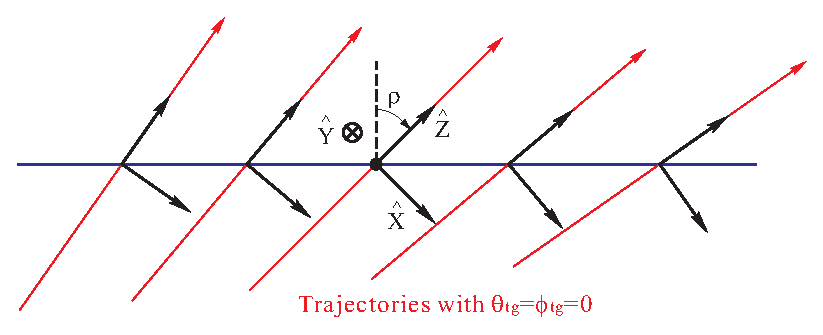
\includegraphics[scale=0.8]{figs/fcs}
  \end{center}
  \caption[Focal coordinate sytem]%
  {Focal coordinate system.}
  \label{fig:fcs}
\end{figure}

% matrix,
% mid-plane symmetry
%
\subsection[Optimization Procedure]{Optimization Procedure}

The DCS variable $x_{det}$, $y_{det}$, $\theta_{det}$, $\phi_{det}$ are
directly measured in experiment, and transformed to focal plane variables
$x_{fp}$, $y_{fp}$, $\theta_{fp}$, $\phi_{fp}$.
%To reconstruct the target variables, we apply a matrix on the focal plane variables.
The optics matrix method provides a point-to-point mapping between focal plane
variables and the target variables, $\theta_{tg}$, $\phi_{tg}$, $y_{tg}$ and $\delta$.

In the optics calibration, the $x_{tg}$ is always set to be zero, and an extended target
correction depend on $beam_{x}$ is applied to $\theta_{tg}$ and $\delta$ in reconstruction.

The first order of optics matrix can be expressed as:

\begin{equation} \label{1st_order_matrix}
  \left(
  \begin{matrix} \delta \\ \theta \\ y \\ \phi \end{matrix}
	\right)_{\mathrm{tg}} = \left(
	\begin{matrix}
	  \left<\delta|x\right> & \left<\delta|\theta\right> & 0 & 0 \\
	  \left<\theta|x\right> & \left<\theta|\theta\right> & 0 & 0 \\
	  0 & 0 & \left<y|y\right> & \left<y|\phi\right> \\
	  0 & 0 & \left<\phi|y\right> & \left<\phi|\phi\right>
	\end{matrix}
  \right)
\left(\begin{matrix} x \\ \theta \\ y \\ \phi \end{matrix}
  \right)_{\mathrm{fp}}.
\end{equation}

The optics matrix used in experiment has a more complicated form: a set of tensors
$D_{jkl}$, $T_{jkl}$, $Y_{jkl}$ and $P_{jkl}$ transform the focal plane variables to
target plane variables as:

\begin{align}
\delta = \sum\limits_{j,k,l} D_{jkl} \theta_{fp}^{j} y_{fp}^{k} \phi_{fp}^{l} \\
\theta_{tg} = \sum\limits_{j,k,l} T_{jkl} \theta_{fp}^{j} y_{fp}^{k} \phi_{fp}^{l} \\
y_{tg} = \sum\limits_{j,k,l} Y_{jkl} \theta_{fp}^{j} y_{fp}^{k} \phi_{fp}^{l} \\
\phi_{tg} = \sum\limits_{j,k,l} P_{jkl} \theta_{fp}^{j} y_{fp}^{k} \phi_{fp}^{l}
\end{align}

where the tensors  $D_{jkl}$, $T_{jkl}$, $Y_{jkl}$ and $P_{jkl}$ are polynomials in $x_{fp}$.
For example:

\begin{align}
\delta = \sum\limits_{j,k,l} D_{jkl} \theta_{fp}^{j} y_{fp}^{k} \phi_{fp}^{l} \\
D_{jkl} = \sum\limits_{i=0} C_{i,j,k}^D x_{fp}^i 
\end{align}

where $C_{i,j,k}^T$ are the optics matrix elements of $\theta_{tg}$.
The optics matrix elements power of  $x_{fp}$, $\theta_{fp}$, $y_{fp}$, $\phi_{fp}$ is 
up to third order. The optics optimization is a method to determine the optics matrix
elements using the optics calibration data. The optimization procedure is described in 
the next section.

\subsection{Experimental and Optimization Procedure}
The optics calibration requires sets of data with wide coverage on the entire acceptance
of spectrometer, which includes $\delta$ for momentum, $\theta_{tg}$ and $\phi_{tg}$ for solid
angle and $y_{tg}$ for reaction position. 
These target variables for calibration data should be precisely determined by methods including:
survey of sieve-slit collimator and spectrometer for $\theta_{tg}$ and $\phi_{tg}$, survey of foil target 
for $y_{tg}$, and some well-known physics process like elastic scattering for $\delta$.

To optimize $\theta_{tg}$, $\phi_{tg}$ and $y_{tg}$, a multi-foil optics target is used,
with a fixed energy, raster-off electron beam. The 7 carbon foils of the optics target
are aligned along the beam line to cover the $y_{tg}$ acceptance, from $z=$-12 cm to $z=$+12 cm,
with a separation of 4 cm. So the $z_{react}$ can be determined by $z$ coordinate of survey result of the 
target foils. The $x_{beam}$ and $y_{beam}$ of interaction point in HCS coordinate can
be determined by BPM. A sieve slit collimator is inserted before the entrance of first quadrupole
of the spectrometer. A figure of the sieve slit is shown in Figure ?.
The holes on the sieve slit are placed in a grid pattern, and the large holes are used to determine
the orientation of the image at the focal plane. 

The in-plane angle $\phi_{tg}$ and out-of-plane angle $\theta_{tg}$ for each sieve-slit hole can be
expressed as:

\begin{align}
\phi_{tg}   =
\frac{y_{sieve}+D_y-x_{beam}\cos\theta_0+z_{react}\sin\theta_0}{L-z_{react}\cos\theta_0-x_{beam}\sin\theta_0}\\
\theta_{tg} = \frac{x_{sieve}+D_x+y_{beam}}{L-z_{react}\cos\theta_0-x_{beam}\sin\theta_0}
\end{align}

where $\theta_0$ is the spectrometer central angle, $D_x$ and $D_y$ are the vertical and horizontal
mis-pointing of the spectrometer central ray from the HCS origin, $L$ is the distance from the
TCS origin to the sieve slit. $\theta_0$, $L$, $D_x$ and $D_y$ can be determined from survey
of spectrometer and sieve slit. The spatial coordinates $x_{tg}$ and $y_{tg}$ can be expressed by:

\begin{align}
x_{tg} = x_{sieve} - L \theta_{tg} \\
y_{tg} = y_{sieve} - L \phi_{tg} 
\end{align}

The momentum calibration use the elastic scattering to determine the momentum of the detected
particle. It requires precise measurement of spectrometer central momentum and beam energy.
The scattering momentum can be expressed as:

\begin{equation}
P(M,\theta) = E' = \frac{E}{1+\frac{E}{M}(1-\cos\theta)}
\end{equation}

where E is the beam energy, M is the target mass and $\theta$ is the scattering angle.
Because the solid angle acceptance covers a wide $\theta_{tg}$ and $\phi_{tg}$ range,
the scattering angles of the electrons passing through different sieve holes are different.
The elastic peak will be broadened and this effect becomes larger for lighter target nucleus.
So a new variable $\delta_{kin}$ is defined to remove the angular dependence of $\delta$ :

\begin{equation}
\delta_{kin} = \delta - \frac{P(M,\theta_{scat})-P(M,\theta_0)}{P0}
\end{equation}

where the scattering angle $\theta_{scat}$ and $\theta_0$ is the central angle of the spectrometer. 
To cover the $\delta$ acceptance of the spectrometer, several different central momentum $P_0$ values
are set during the optics calibration, which is called "delta scan".

The scattered electrons will pass through target foils and several windows before entering spectrometer,
so the energy loss of the scattered electrons due to radiative effect is considered as a correction to
$\delta$.

For optimization of optics matrix, the target variables  $\delta$, $\theta_{tg}$, $\phi_{tg}$ and $y_{tg}$
calculated from survey or elastic scattering peak are taken as the true value.

\begin{equation}
\sigma^2(x) = \sum\limits_{s=1}^{N}  (x^{recon} - x^{survey})^2 
\end{equation}

where $N$ is total number of events measured for optics calibration, x can be any target variables
$\delta$, $\theta_{tg}$, $\phi_{tg}$ and $y_{tg}$, $x^{recon}$ is the target variable 
reconstructed by the optics matrix, $x^{survey}$ is the reference target variable calculated from
survey results and elastic scattering peak. 
The optimization begin with an initial optics matrix generated by magnetic field simulation SNAKE.
The core of the optimization package is the TMinuit package of ROOT.
The package also contain scripts to make graphic cuts and select events for optimization.

\subsection[Optics Results]{Optics Results}
In this section, the optimization results are discussed. The data collected with beam energy 1.1 GeV
at $\theta_0$ = 14.6 degree is taken as an example.

The angular components of the optics matrix are optimized first.
The optimized matrix is used to reconstruct the target variables. The sieve pattern is generated by
the projection of the reconstructed $\theta_{tg}$ and $\phi_{tg}$ from the interaction point to the sieve
slit plane. The sieve pattern for the 1.1 GeV data is shown in Figure ?.
The nominal position of the sieve holes are indicated by the cross points of the grids in the plots.
The resolution of $\theta_{tg}$ and $\phi_{tg}$ are $~1\times 10^{-4}$ mrad and $~ 0.5 \times 10^{-4}$ mrad.

Next step is the momentum calibration. The $\delta_{kin}$ calibration results for 1.1 GeV data are
shown in Figure ?. The nominal position of the $\delta_{kin}$ are indicated by magenta lines for each
delta scan configuration. The resolution of each $\delta_{kin}$ peak is $~ 2 \times 10^{-4}$. 

The $y_{tg}$ calibration results are shown in Figure ?. The nominal position of the optics foils are
indicated by red lines for each foil. The resolution of $y_{tg}$ of foils are $~1 mm$.


%%%%%%%%%%%%%%%%%%%%%%%%%%%%%%%%%%%%%%%%%%%%%%%%%%%%%%%%%%%%%%%%%%%%%%%%
\section{Acceptance of HRS spectrometer}

Because the limited aperture of HRS spectrometer, the spectrometer can only detect scattered electrons
in a certain range of $\theta_{tg}$, $\phi_{tg}$, $\delta$ and $y_{tg}$.
The acceptance of spectrometer can be defined as the window of $\theta_{tg}$, $\phi_{tg}$, $\delta$ and $y_{tg}$ (The foil target only has acceptance in first three variables, the $y_{tg}$ acceptance
is used only for extended target) in which scattered electrons can pass through all the magnets of the
spectrometer and  be detected at focal plane.
In ideal case, the spectrometer would accept all the particles if they are inside the aperture of
spectrometer and reject particles outside aperture.
But in reality, the spectrometer's geometrical aperture is more complicated than a hypercube of 
the five target variables, and the multiple scattering and resolution of the VDC wire chambers will smear
out the boundaries.
So a more proper definition of acceptance is a probability function depend on target variables,
acc($\theta_{tg}$, $\phi_{tg}$, $\delta$, $y_{tg}$). The value  is the 
probability of scattered electrons with certain target variables can reach focal plane.

\subsection{SAMC simulation}
A Monte Carlo simulation package called the Single Arm Monte Carlo (SAMC), is used to study 
the acceptance of spectrometer. The SAMC was originally written in Fortran by  A. Deur and converted
into ROOT/C++ by Huan Yao. A detailed description of the SAMC is given below:

\begin{itemize}
\item Trial events are generated at the target with uniform distribution in $(\delta,\theta_{tg},\phi_{tg},y_{tg})$.
\item
Since each electron pass through target and a few windows, the radiative effects due to the bremsstrahlung
and ionization, and multiple scattering are taken into consideration (The windows and other materials are
listed below in table ?).

\item The SAMC uses a set of forward propagation matrix which is generated by SNAKE simulation
and MUDIFI fit package. The position of each event is checked at every aperture in the spectrometer.

\item The events pass through all the aperture cuts in spectrometer are transported to VDC wire plane.
They are randomly smeared according to the VDC resolution $\sigma_x$ = $\sigma_y$ = 100 $\mu m$,
$\sigma_\theta$ = $\sigma_\phi$ = 0.3 mrad. 

\item All the events reach the focal plane are reconstructed back to the target with reverse matrix.

\end{itemize}

\subsection{Acceptance}

The acceptance used in this analysis are four dimensional acceptance. The projection of the acceptance
on $dp$ and $y_{tg}$ is shown in Figure ?. 

\subsection{Overlap smoothing of acceptance}
Because the forward matrix cannot perfectly describe the magnet field at the edge, the acceptance
at the edge of $dp$ needs to be corrected properly. In experiment, a serial of runs with 
?????????????????????????????

%%
%%%%%%%%%%%%%%%%%%%%%%%%%%%%%%%%%%%%%%%%%%%%%%%%%%%%%%%%%%%%%%%%%%%%%%%%
%\section{BCM calibration}
%Beam Current Monitor (BCM) is done in two steps: 
%
%\subsection{EPICS calibration}
%EPICS calibration provides the absolute beam current measurement.
%This calibration use OLO2 caivity monitor and Faraday cup at the accelerator
%injector section during the calibration run.
%
%During the calibration run, the electron beam only goes to Hall A. The $I_{Faraday}$,
%$I_{OLO2}$ and the average voltage level of BCM cavities (upstream $V^u$ and downstream $V^d$)
%are measured simultaneously. 
%
%\begin{table}[tb!]
%\begin{tabular}{ccr}
%\hline
%$I_{OLO2}$($\mu$A)            & $I_{Faraday}$($\mu$A)         & $\frac{I_{OLO2}}{I_{Faraday}}$-1(\%) \\ \hline
%59.491 $pm$ 0.245             & 59.318 $\pm$ 0.177            & 0.29                                 \\
%39.160 $pm$ 0.049             & 39.048 $pm$ 0.068             & 0.29                                 \\
%19.594 $pm$ 0.033             & 19.472 $pm$ 0.012             & 0.62                                 \\
%10.810 $pm$ 0.039             & 10.723 $pm$ 0.051             & 0.81                                 \\
%5.038 $pm$ 0.007              & 5.034 $pm$ 0.01               & 0.06                                 \\
%2.171 $pm$ 0.008              & 2.164 $pm$ 0.005              & 0.33                                 \\
%1.017 $pm$ 0.002              & 1.019 $pm$ 0.017              & 0.27                                 \\
%0.542 $pm$ 0.002              & 0.549 $pm$ $6\times 10^{-4}$  & 1.20                                 \\
%0.259 $\pm$ $4\times 10^{-4}$ & 0.263 $\pm$ $5\times 10^{-5}$ & 1.50                                 \\ \hline
%\end{tabular}
%\end{table}
%
%\begin{table}[tb!]
%\begin{tabular}{ccr}
%\hline
%BCM Scaler & Scaler Constant   & Offset \\ \hline
%U1         & 2372.4 $\pm$ 2.4  & 362.5  \\
%U3         & 7294.5 $\pm$ 7.5  & 350.2  \\
%U10        & 22067  $\pm$ 225  & 442.6  \\
%D1         & 2427.9 $\pm$ 2.2  & 160.1  \\
%D3         & 7517.4 $\pm$ 8.7  & 126.7  \\
%D10        & 23485  $\pm$ 286  & 321.1  \\ \hline
%\end{tabular}
%\end{table}
%
%The beam charge can be expressed as:
%\begin{equation}
%Q(\mu \C) = \frac{\mathrm{Scaler}_{U3} - \mathrm{Offset_{U3} \times T}{C_{U3}}
%\end{equation}

%%%%%%%%%%%%%%%%%%%%%%%%%%%%%%%%%%%%%%%%%%%%%%%%%%%%%%%%%%%%%%%%%%%%%%%%
\section{Livetime}
There are two types of deadtime: computer deadtime and electronic deadtime.

\subsection{Electronic Deadtime}
When particles generate signals at the detectors, these signals are sent to the TDC and ADC electronics.
The TDC and ADC cannot process singals continuously: when an event is immediately followed by another
before the detector gate is ready for the latter. The gate opening time is $~$ 100 ns for both LHRS and RHRS.



\subsection{Computer Deadtime}
The computer deadtime is

%%%%%%%%%%%%%%%%%%%%%%%%%%%%%%%%%%%%%%%%%%%%%%%%%%%%%%%%%%%%%%%%%%%%%%%%
\section{PID Efficiency}


%%%%%%%%%%%%%%%%%%%%%%%%%%%%%%%%%%%%%%%%%%%%%%%%%%%%%%%%%%%%%%%%%%%%%%%%
\section{Tracking Efficiency}

Vertical Drift Chambers (VDC) detect hits of scattered electrons and reconstruct tracks through track
reconstruction algorithm.
Under normal conditions, each event leaves only one track in the VDC, but in certain case an event
can have zero track or multi-track.
The inefficiency of VDC wire or failure of track reconstruction may result in zero track events.
In most of the case, the wire inefficiency is less than 0.1\%.
The wire inefficiency cannot be separated from the tracking efficiency and is convoluted into 
the multi-track efficiency.
A multi-track event means an event  with 2 or more tracks reconstructed by VDC.
It can happen when several electron generated secondary particles passing through VDC simultaneously,
or there is noise in VDC.

For most of runs in CSR experiment, the event rate is below 10 kHz and only a small fraction of events ha
s multi-track. For kinematics settings with higher trigger rate, the fraction of multi-track events is also
higher: there are some runs with trigger rate higher than 10 kHz, and the multi-track events
takes more than a few percent in total event number. So a strict treatment is necessary for these runs,
the multi-track events must be examined carefully to determine whether or nor there is a good track among all
the reconstructed tracks.
%We can use the PID and acceptance cut to select a clean sample, and use the energy deposit
%around the each track's trajectory in lead glass to check if an event contains a good track.

The tracking efficiency can be defined as the ratio between good events number with a successful track reconstruction
and total events number.

\begin{equation}
\varepsilon_{VDC} = \frac{N_{good}}{N_{total}}
\end{equation}

where $N_{good}$ is the number of events with events with a successful track reconstruction and checked
by the energy deposit on lead glass calorimeter, $N_{total}$ is the number of events that pass the acceptance
cut and PID cut.

Because the check of multi-track event is very time consuming, in analysis of production runs, we usually only
use events with a single track, so a correction for the loss of multi-track events is necessary:
We redefine the tracking efficiency as the ratio between number of good single track events and number of all
good events: 

\begin{equation}
\varepsilon_{VDC} = \frac{N_{goodsingletrack}}{N_{goodsingletrack}+N_{goodmultitrack}}
\end{equation}

where the $N_{singlegoodtrack}$ is the number of events with good single-track events in the sample,
$N_{multigoodtrack}$ is the number of multi-track events with at least one good track in the sample.

A multi-track event is considered as good event if :
(a) at least one track inside the normal acceptance cut used for this analysis:
$|dp|\leq$ 3.5\%, $|\theta_{tg}| \leq$ 40 mrad, $|\phi_{tg}| \leq$ 20 mrad;
(b) energy deposited in the calorimeter of this track satisfies the PID cuts.
Figure xx shows the acceptance cut used in this analysis.

To get the energy deposition of a track in calorimeter, we need to project the
track trajectory forward onto calorimeter (Because some of the blocks of the NaI calorimeter in LHRS was
not responsive during the experiment, this tracking efficiency is only studied on
RHRS, and then applied to LHRS).
Figure xx shows the distribution of energy deposition in 2 layers of calorimeter (shower and preshower)
for two-tracks events. The  
%%%%%%%%%%%%%%%%%%%%%%%%%%%%%%%%%%%%%%%%%%%%%%%%%%%%%%%%%%%%%%%%%%%%%%%%
\section{Center-of-bin Correction}

With an angular cut of $|\theta_{tg}|\leq$ 40 mrad,  $|\phi_{tg}| \leq$ 20 mrad, as mentioned previously,
the cross section measured at a certain central spectrometer angle actually is the average of cross section
in the range of acceptance. Because the cross section varied non-linearly within the finite bin of the acceptance,
a center-of-bin correction is applied to correct this finite acceptance effect.

If we know the cross sections very well, for example, the carbon/proton elastic cross section,
we can use the parametrized cross section from phase shift calculation to get a center-of-bin factor, $C_a$:

\begin{equation}
C_a = \frac{\sigma_c}{ \frac{\int \sigma(\theta,\phi,\delta) \times
Acc(\theta,\phi,\delta)}{\int_{\theta,\phi,\delta}Acc(\theta,\phi,\delta) }}
\end{equation}

where $\sigma_c$ and $\sigma(\theta,\phi)$ are the calculated cross sections at the center and at a certain bin ($\theta,
\phi, \delta$) of the acceptance.

For the case of quasi-elastic scattering region, we don't known the exact cross section, the correction is performed
with a calculated cross section from F1F209 model.

%%%%%%%%%%%%%%%%%%%%%%%%%%%%%%%%%%%%%%%%%%%%%%%%%%%%%%%%%%%%%%%%%%%%%%%%
\section{Radiation Correction}
%%\label{C5S4}
The cross section in equation ? is derived to lowest order in fine-structure
constant $\alpha$ including only the amplitude due to exchange of single virtual photon between 
the incident electron and nucleon, which is known as Born approximation. The cross section measured
in electron scattering in experiments have large contribution from higher order process and the 
straggling effect. So the raw cross section need to be corrected to extract Born cross section.
This correction is called "radiative correction". 
In this section, a summary of theory and application of radiative correction is given.

Feynman diagrams of the second order and third order processes are shown in Figure ?.

Will talk about follow topics in this section:
(1) calculate the elastic tradiative tail; (2) quasi-elastic radiative corrections;
(3) radiative correction to elastic data;

\subsection{Elastic Radiative Tail}
Following the formalism of Mo and Tsai and Stein, the cross section for the elastic radiative tail is:

\begin{equation}
\sigma_{el tail} = (\sigma_{int} + \sigma_{ext} + \sigma_{coll}) \cdot F_{soft}
\end{equation}

where $\sigma_{int}$, $\sigma_{ext}$, $\sigma_{coll}$ and $F_{soft}$ represent the internal bremsstrahlung, external bremsstrahlung
, collisional loss and soft photon correction.

\subsubsection{Internal Bremsstrahlung}
When the bremsstrahlung photon emission is during the collision, this process is called internal bremsstrahlung. The
internal bremsstrahlung cross section for elastic scattering can be calculated exactly (to lowest order order of
$\alpha$) is we assume one-photon exchange.


\begin{equation}
\sigma_{int} = \int B_{\mu\nu} T_{\mu\nu} d\Omega_k,
\end{equation}

where $B_{\mu\nu}$ is the internal bremsstrahlung tensor and $T_{\mu\nu}$ is the lepton tensor.



\subsection{Radiative Corrections for Quasi-elastic Data}

\begin{equation}
t_r = \left(\frac{\alpha}{b\pi} \right) \left[ \ln\left(\frac{Q^2}{m_e^2}\right)-1 \right]
\end{equation}

\begin{equation}
\begin{split}
\left( \frac{d^2\sigma}{d\Sigma d\omega} \right)_{exp}  =  \left(\frac{R\Delta E}{E_i}\right)^{bt'_b}
\left(\frac{\Delta E}{E_f}\right)^{bt'_a} \left[1 - \frac{\xi/\Delta E}{1-b(b(t'_a + t'_b))} \right] \tilde{\sigma}(E_i,
E_f) \\
 + \int_{E_{i min}}^{E_i - R\delta E} \tilde{\sigma}(E'_i, E_f) \left( \frac{E_i - E'_i}{RE_f} \right)^{bt'_a} \left(
\frac{E_i - E'_i}{E_i}\right)^{bt'_b} \\
 \times \left[ \frac{bt'_b}{E_i - E'_i} \phi \left( \frac{E_i-E'_i}{E_i} \right) + \frac{\xi}{2(E_i - E'_i)^2} \right]
dE'_i  \\
 + \int_{E_f + \delta E}^{E_{f max}} \tilde{\sigma} (E_i, E'_f) \left( \frac{E'_f - E_f}{E'_f} \right)^{bt'_a} \left(
\frac{R(E'_f - E_f)}{E_i} \right)^{bt'_b} \\
 \times \left[ \frac{bt'_a}{E'_f-E_f} \phi\left(\frac{E'_f - E_f}{E'_f}\right)+\frac{\xi}{2(E'_f - E_f)^2} \right] dE'_f ,
%
\end{split}
\end{equation}

\subsection{Radiative Corrections for Elastic Data}
The radiative correction to the elastic peak has been well studied.
The relation between cross section measured in experiment and the Born cross section is:

\begin{equation}
\left(\frac{d\sigma}{d\Omega}\right)_{exp} = (1+\delta) \left( \frac{d\sigma}{d\Omega} \right)_{Born}
\end{equation}

where $\delta$ is the radiative correction. Higher order corrections are taken into account by replacing
$1+\delta$ with $e^{\delta}$.

The expression of $\delta$ is sum of the external and internal terms.

The internal term include contribution from internal bremsstrahlung, vacuum polarization and nucleus recoil and photon emission: 

\begin{multline}
%\begin{equation}
%\begin{split}
\delta_{int}  =
%\frac{-\alpha}{\pi} \left(
\frac{28}{9} - \frac{13}{6} \ln \left( \frac{Q^2}{m^2_e} \right)  +
\left( \ln \left( \frac{Q^2}{m^2_e} \right) - 1 + 2Z \ln \left( \frac{E_i}{E_f} \right) \right) \\
\times \left[ 2\ln \left( \frac{E_i}{\Delta E} \right) - 3\ln \left( \frac{E_i}{E_f} \right) \right]  \\
-\Phi \left( \frac{E_f-E_i}{E_f} \right)
- Z^2 \ln \left( \frac{E_t}{M_t} \right)
+ Z^2 \ln \left( \frac{M_t E_f}{E_i \Delta E} \right)
\left( \frac{1}{\beta_t} \ln \left( \frac{1+\beta_t}{1-\beta_t} \right) -2 \right) \\
+ \frac{Z^2}{\beta_t} \left\{ \frac{1}{2} \ln\left( \frac{1+\beta_t}{1-\beta_t} \right) \ln\left( \frac{E_t+M_t}{2M_t} \right) 
-\Phi \left[ -\left( \frac{E_t-M_t}{E_t+M_t}\right) \left(  \frac{1+\beta_t}{1+\beta_t} \right)^{\frac{1}{2}} \right]
\right\} \\
- Z \left[ \Phi\left(-\frac{E_t-E_f}{E_f}\right) -\Phi\left( \frac{M_t(E_t-E_f)}{2E_iE_t-M_tE_f} \right)
+ \Phi \left( \frac{2E_i(E_t - E_f)}{2E_i E_t - M_t E_f} \right)  
%+\ln | \frac{2E_i E_t - M_t E_f}{E_f(M_t - 2E_i)} | \ln left( \frac{M_t}{2E_i} \right)
\right]
%\right)
%\end{split}
%\end{equation}
\end{multline}


%%%%%%%%%%%%%%%%%%%%%%%%%%%%%%%%%%%%%%%%%%%%%%%%%%%%%%%%%%%%%%%%%%%%%%%%
\section{Experimental Cross Section}
The goal of E05-110 experiment is to measure the longitudinal and transverse response functions, and 
extract Coulomb Sum to test Coulomb Sum Rule(CSR). To obtain Coulomb Sum with required precision,
it is important to extract the cross section while minimizing the uncertainties. The raw experimental cross
section can be written as:

\begin{equation}
\frac{d\sigma}{d\Sigma d\omega} = \frac{N_{cut}}{(Q/e) \cdot t_{LT} \cdot Acc \cdot \varepsilon \cdot N_{tg}}
\frac{1}{\Delta E' \Delta \Omega}
\end{equation}

\begin{itemize}
\item $N_{cut}$ is the number of events within all electron cut in one bin.

\item $Q/e$ is the number of incident electrons. $Q$ is the total charge which is read from BCM scaler.
$e$ is the charge of a single electron.

\item $t_{LT} = T_{1(3)}/T_{1(3)raw}$ is the Livetime of the detector.
$T_{1(3)}$ are the main trigger event type for right(left) arm.

\item $Acc$ is the spectrometer's acceptance determined from Monte Carlo simulation (SAMC).

\item $\varepsilon$ is the total efficiency $\prod_i \varepsilon_i$ for all detectors:
VDC, scintillator, gas Cerenkov, shower and preshower;

\item $N_{tg}$ is the number of the target particles.  $L\rho$ is the target thickness (in unit of g/cm$^3$),
$N_a = 6.02 \times 10^{23}$ is the Avagadro's number. A is the atomic number of the target.

\begin{equation}
N_{tg} = \frac{L\rho N_a}{A}
\end{equation}

\item $\Delta E = P_0 dp$ is the energy width (in unit of MeV) for the given momentum bin.

\item $\Delta \Omega = \Delta \theta \Delta \phi$ is the solid angle defined by the width of acceptance cuts in
$\theta_{tg}$ and $\phi_{tg}$. In this analysis, cut in $\theta_{tg}$ and $\phi_{tg}$ are $\Delta \theta$ = 80 mrad,
and $\Delta \phi$ = 40 mrad.

\end{itemize}

%%%%%%%%%%%%%%%%%%%%%%%%%%%%%%%%%%%%%%%%%%%%%%%%%%%%%%%%%%%%%%%%%%%%%%%%
\section{Density effect}

The $^{4}$He is in high pressure gas state, and the $^{208}$Pb is
kept in liquid hydrogen. For fluid targets, the local heating generated
by beam current may result in decrease of density near the beam trajectory. 
This localized effect cannot be detected by sensor devices.
This density fluctuation effect can be measured by investigating the 
linearity between the event yield and the beam current using elastic
scattering data.

The density fluctuation depends on two parameters, beam current and beam
size. A higher beam current/smaller beam size will decrease the target
density.  Due to the configuration of the cryogenic target, that the 
cooling enter the target from the top and exit from the bottom, the 
vertical beam size has less effect on target density.

And it is interesting to see the difference between the two kinds of
cryogenic target: the density of $^{4}$He target decrease linearly as
beam current grows, while the liquid hydrogen target has a changing 
slope. The density fluctuation is less than 5\% for this analysis.


%%%%%%%%%%%%%%%%%%%%%%%%%%%%%%%%%%%%%%%%%%%%%%%%%%%%%%%%%%%%%%%%%%%%%%%%
%%\section{Rosenbluth Separation}
%%\label{C5S5}



%\cite{*}

%%%%%%%%%%%%%%%%%%%%%%%%%%%%%%%%%%%%%%%%%%%%%%%%%%%%%%%%%%%%%%%%%%%%%%
% -*-latex-*-

%\appendix
%% -*-latex-*-

\chapter{Appendix A}

\newpage
\cleardoublepage

%%%%%%%%%%%%%%%%%%%%%%%%%%%%%%%%%%%%%%%%%%%%%%%%%%%%%%%%%%%%%%%%%%%%%%
% -*-latex-*-


\cleardoublepage
\pdfbookmark[0]{Bibliography}{Bibliography}
% -*-latex-*-

%% This defines the bibliography file (main.bib) and the bibliography style.
%% If you want to create a bibliography file by hand, change the contents of
%% this file to a `thebibliography' environment. For more information, see
%% section 4.3 of the LaTeX manual.

\begin{singlespace}
\bibliography{main}
\bibliographystyle{plain}
\end{singlespace}

%%%%%%%%%%%%%%%%%%%%%%%%%%%%%%%%%%%%%%%%%%%%%%%%%%%%%%%%%%%%%%%%%%%%%%
% -*-latex-*-

\cleardoublepage

\end{document}

%%%%%%%%%%%%%%%%%%%%%%%%%%%%%%%%%%%%%%%%%%%%%%%%%%%%%%%%%%%%%%%%%%%%%%
% -*-latex-*-
